% Stanford University PhD thesis style -- modifications to the report style
% This is unofficial so you should always double check against the
% Registrar's office rules
% See http://library.stanford.edu/research/bibliography-management/latex-and-bibtex
% 
% Example of use below
% See the suthesis-2e.sty file for documentation
%
\documentclass{report}
\usepackage{suthesis-2e}
\dept{Physics}

\begin{document}
\title{It's ok to be selfish \ldots if you're the Higgs\\
       because why stop at one when you can have \emph{two}?}
\author{Nicole Hartman}
\principaladviser{Su Dong}
\firstreader{Michael Kagan}
\secondreader{Patricia Burchat}
\thirdreader{Michael Peskin} %if needed
 
\beforepreface
\prefacesection{Abstract}
This thesis tells you all you need to know about...
\prefacesection{Acknowledgments}
I would like to thank...
\afterpreface

\chapter{Introduction}
\begin{chapquote}{Thomas Khun, \emph{The Structure of Scientific Revolutions}}{Until taught by prolonged exposure that the universe contained anomalous cards, they saw only the types of cards for which previous experience had equipped them. Yet once experience had provided the requisite additional categories, they were able to see all anomalous cards on the first inspection long enough to permit any identification at all \ldots}
\end{chapquote}


\begin{itemize}
	\item Why we expect new physics in the SM
	\item Motivation for HH
	\item Particulars about the 4b final state
	\item Connection to ML
	\item Highlight my work on b-tagging
	\item Thesis organization
\end{itemize}


\textbf{Refs: }
\begin{itemize}
\item Higgs discovery:  \cite{HIGG-2012-27, CMS-HIG-12-028}.
\end{itemize}
\chapter{Theoretical motivation}

\begin{chapquote}{Thomas Khun, \emph{The Structure of Scientific Revolutions}}{Surveying the rich experimental literature from which these examples are drawn makes one suspect that something like a paradigm is prerequisite to perception itself.}
\end{chapquote}

\section{The Standard Model}

SU(3) x SU(2) x U(1) gauge interactions

\begin{figure}
\centering
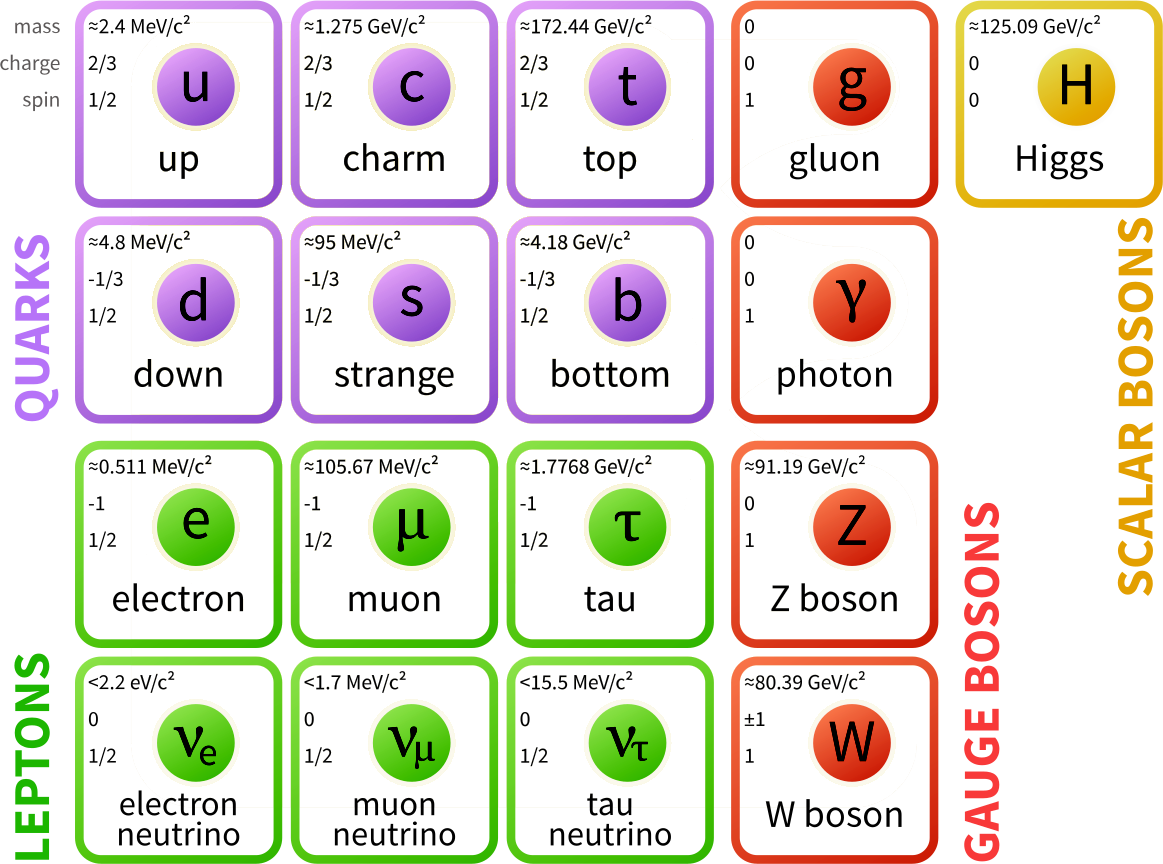
\includegraphics[width=.7\textwidth]{figures/intro/SM-Particles.png}
\caption{\cite{wiki-sm}}
\label{fig:SM-Particles}
\end{figure}

\begin{equation}
\mathcal{L}_{SM} =  - \frac{1}{4} F_{\mu \nu} F^{\mu \nu} + i \bar{\psi} \gamma_\mu D^\mu \psi + \left( y_{ij} \bar{\psi}_i \psi_j + h.c. \right) + |D^\mu \phi|^2 - V (\phi)
\label{eq:sm}
\end{equation}

%I think the

\begin{figure}
\centering
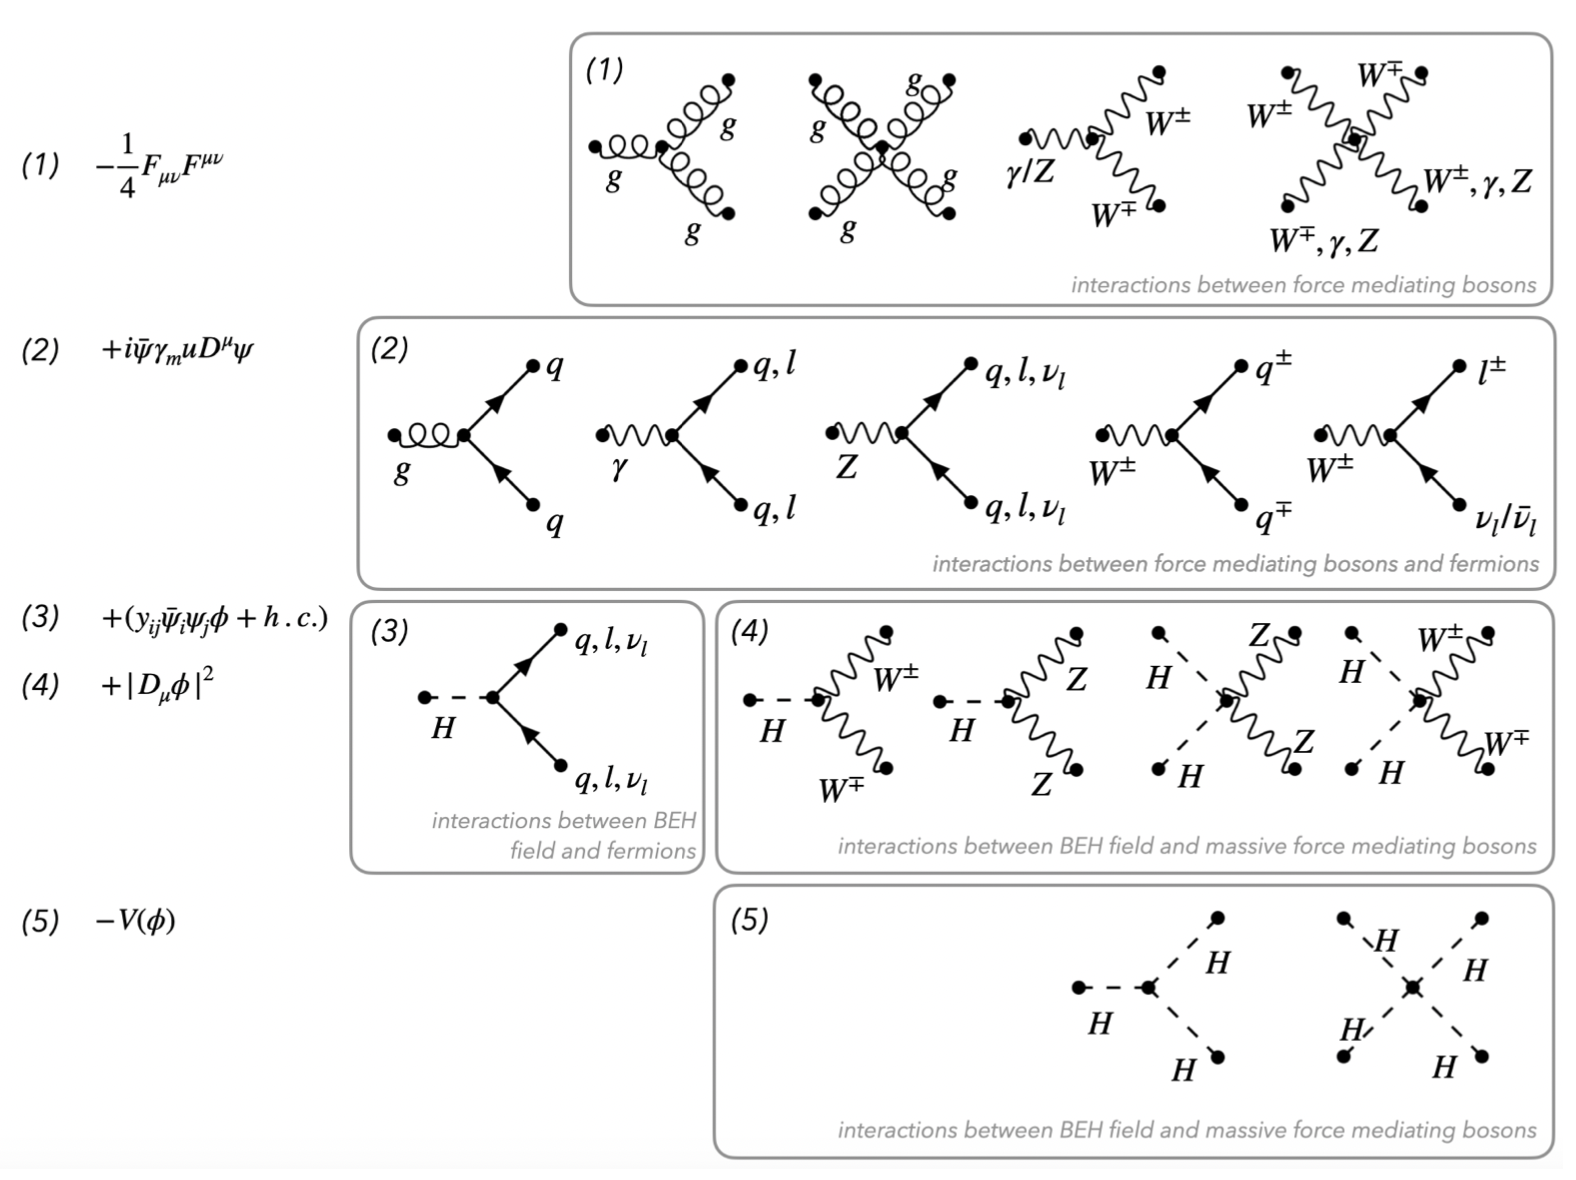
\includegraphics[width=\textwidth]{figures/intro/mel-sm-diagrams.png}
\caption{\cite{Melissa-thesis}}
\label{fig:mel-sm}
\end{figure}

\section{The Higgs mechanism}
I heard from Dale that the pdg is a v good ref for this!!

\section{Effective Field Theories to search for new physics}

\section{Status of the experimental HH results}

\begin{figure}
\centering
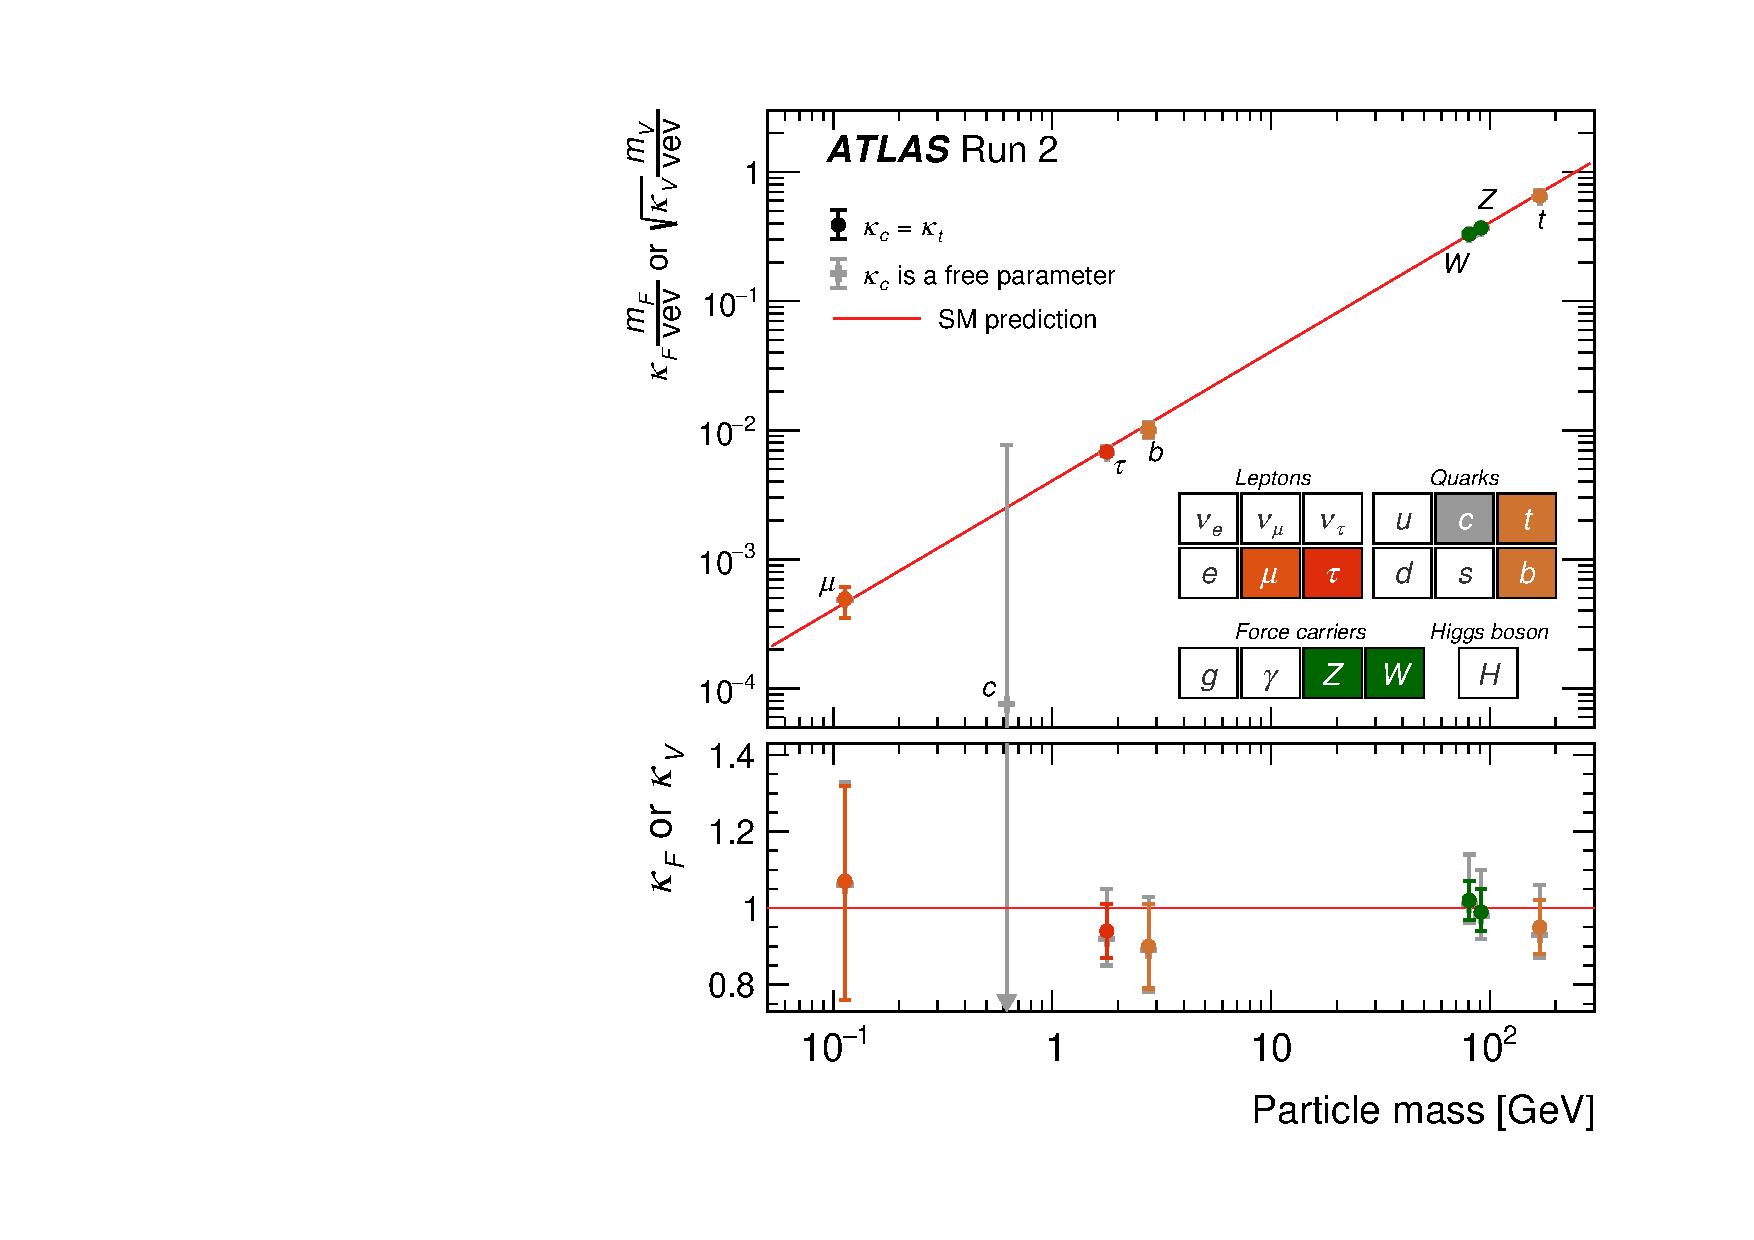
\includegraphics[width=.7\textwidth]{figures/intro/atlas-nature-10yrs/fig_05}
\caption{\cite{2207.00092}}
\label{fig:pcle-mass-atlas}
\end{figure}

\chapter{LHC}
\chapter{ATLAS}
\chapter{Event reconstruction}
\chapter{b-tagging}
\begin{chapquote}{Michael Nielson, \emph{Neural Networks and Deep Learning}}{Technical expertise is the mastery of complexity -- creativity is the mastery of simplicity.}
\end{chapquote}

\section{Introduction}
\label{sec:ftag-intro}

For the physics program of the ATLAS experiment at the Large Hadron Collider (LHC), the identification of jets initiated by $b$-quarks, or $b$-tagging, is a fundamental tool. 
Ensuring its optimal performance is particularly important for the study of the Higgs boson and the top quark \cite{HIGG-2018-04, HIGG-2018-13}, as well as many exotic extensions of the Standard Model with resonances preferentially decaying to heavy quarks \cite{ATLASdijetres}. 


\begin{figure}[htbp]
  \centering
  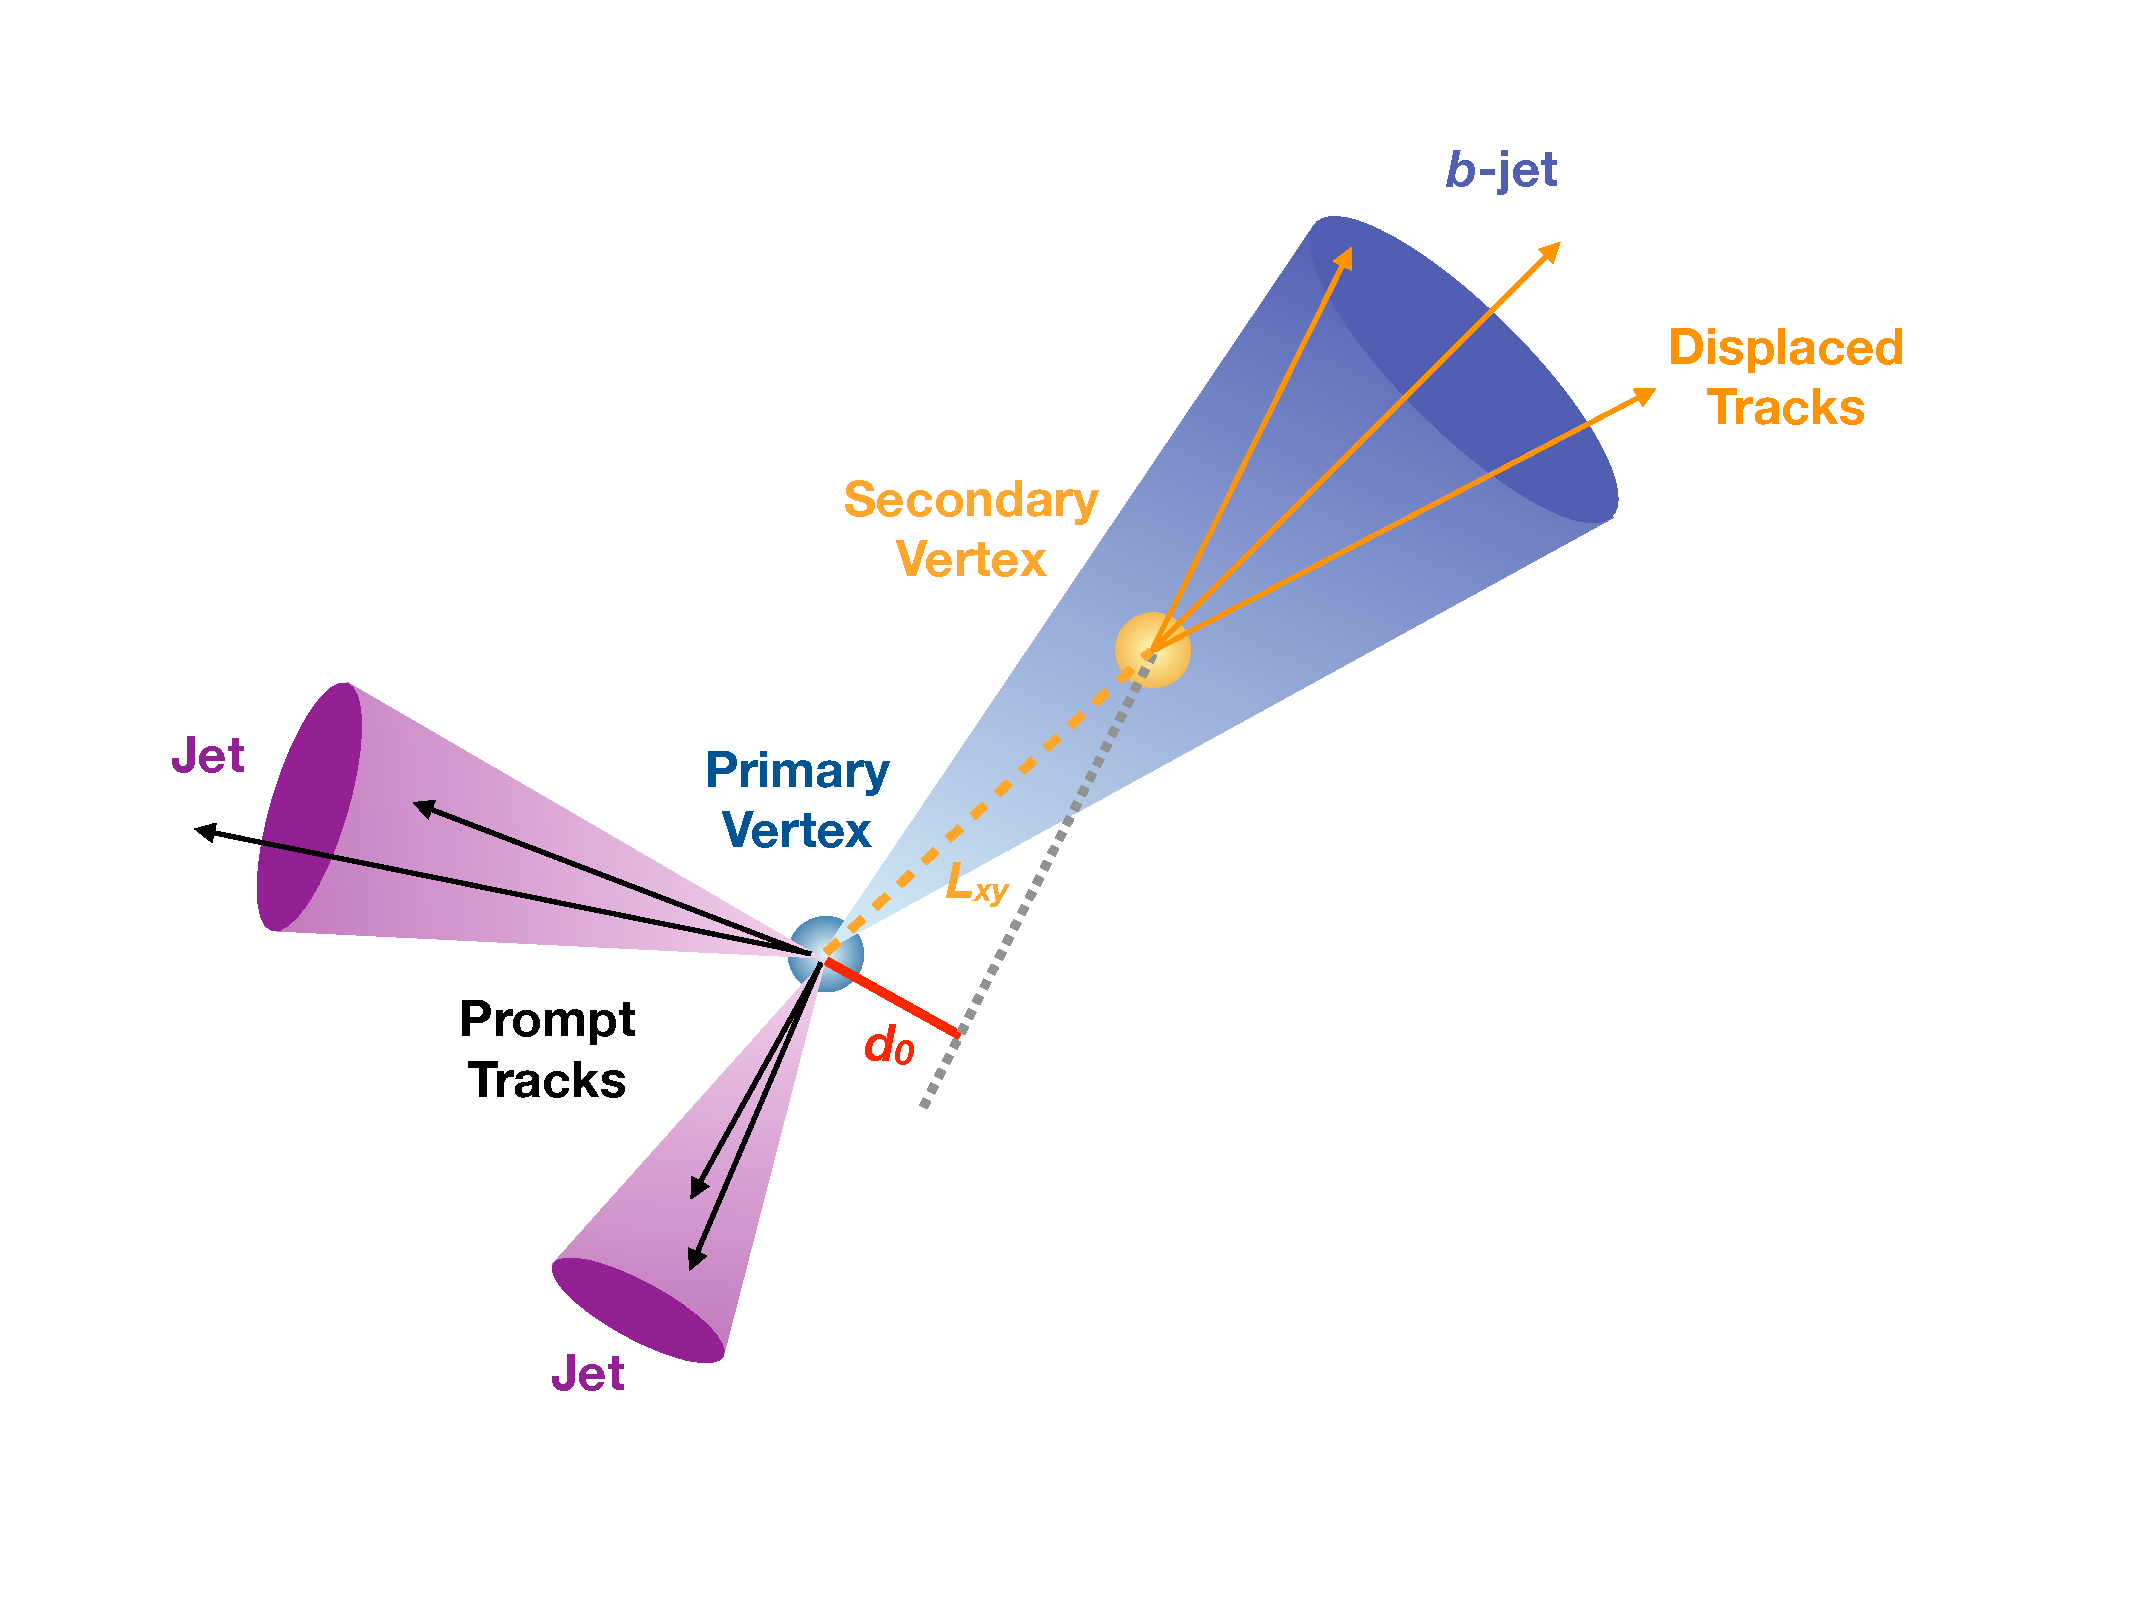
\includegraphics[width=0.7\textwidth]{figures/ftag/b-trig-paper/fig_01}
  \caption{Schematic illustration for the characteristic ``long'' lifetime of a \Pqb-hadron \cite{b-trig-paper}. }
  \label{fig:b-jet-graphic}
\end{figure}

The characteristically long lifetime of hadrons containing $b$-quarks ($b$-hadrons) of the order of 1.5 ps \cite{PDG} leads to two classes of $b$-tagging algorithms: \textit{vertexing} based algorithms which explicitly reconstruct a production point, or vertex, of the $b$-hadron decay displaced from the primary interaction point, and track based algorithms which exploit the displacement of the reconstructed charged particles trajectories (tracks) produced in $b$-hadron decays from the primary interaction point.

%We then use a NN to combine information from these low-level algorithms into a high level tagger and we refer to these collection of algorithm to solve the classification problem of identifying jets containing a $b$-quark as $b$-tagging.

\begin{figure}[htbp]
  \centering
  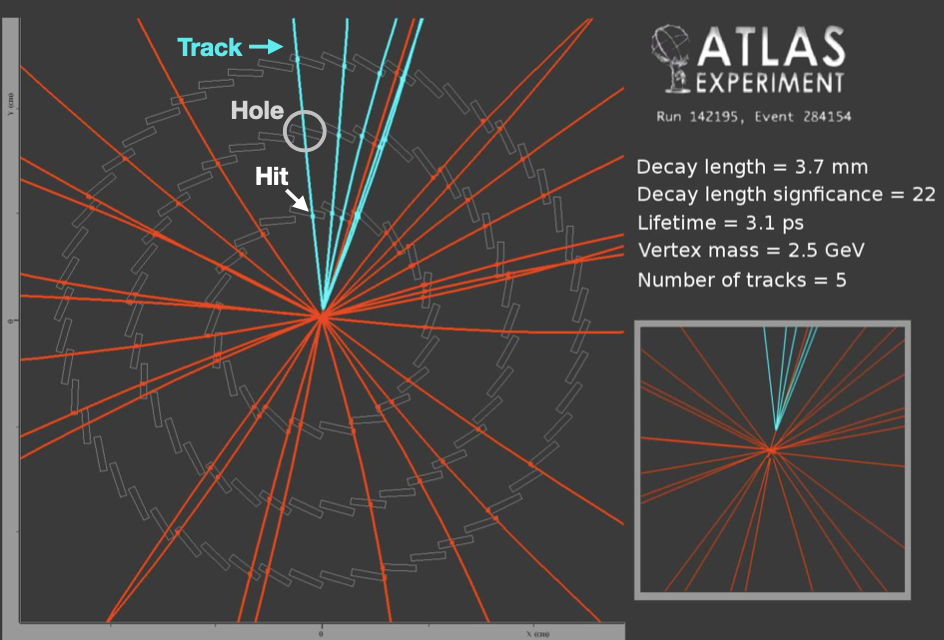
\includegraphics[width=0.9\textwidth]{figures/ftag/b-decay-evt-display-annotated}
  \caption{Illustration of what a b-decay looks like in the ATLAS detector. 
  The cyan colored lines illustrate the tracks from the \Pqb-hadron decay, and in the inset figure you can see the displacement of these tracks from the primary vertex. 
  Only three pixel layers are shown as this is a Run~1 event, and the IBL was not yet installed. \hl{Need to revise older notes to find where this event display came from (or ask Su Dong)}. }
  \label{fig:b-jet-graphic}
\end{figure}

To further set the stage for the problem of interest in this chapter, in \Fig{\ref{fig::jet-displays}} motivates what these weakly decaying hadrons look like in simulation that includes the truth information.
What we have as inputs to flavor tagging are the set of track features in the perigee representation with the IPs defined with respect to the point of closest approach (POCA). \Fig{\ref{fig::jet-displays}} shows these track parameters as we extrapolate out from the PV using the extrapolation equations defined in \Sect{\ref{sec:vertexing}}\footnote{Many thanks to Jonathan Shalomi for the nice track extrapolator code.}.
%The jet displays in \Fig{\ref{fig::jet-displays}} are EMTopo jets passing the standard jet selection cuts, and show all of the reconstructed tracks passing the loosest FTAG preselection. 
These representative images illustrate 
\begin{itemize}
	\item \textbf{\Pqb-jet:} There's a characteristic, tertriary decay of both the B and D hadrons.
	\item \textbf{\Pqc-jet:} There's a weakly decaying D-hadron, but closer to the PV than the weak decays in the \Pqb-jet.
	\item \textbf{light-jet:} Tracks are well collimated with the jet axis and most appear to be originating from the PV, although there are some tracks that that can appear to extrapolate to a point other than the PV.
\end{itemize}

\Tab{\ref{table:decay-length}} shows how often the B and D hadrons decay before the reaching either the first pixel sensor (the IBL) or even the edge of the beam pipe and illustrates that the power of the reconstructing the displaced vertex mostly is coming from the extrapolation.

\begin{table}[h!]
  \centering
    \begin{tabular}{l | l l  } % <-- Alignments: 1st column left, 2nd middle and 3rd right, with vertical lines in between
      {} & \textbf{B-hadron decays before} & \textbf{D-hadron decays before}  \\
      \hline
	Beam pipe &  2.1 \% & 0.3 \% \\
	IBL & 0.94 \% & 0.1 \%
    \end{tabular}
    \caption{Decay length of the weakly decaying hadron for jets in from a semi-leptontic $t\bar{t}$ sample.}
    \label{table:decay-length}
\end{table}

\begin{figure} 
\centering
\vspace{-1cm}
	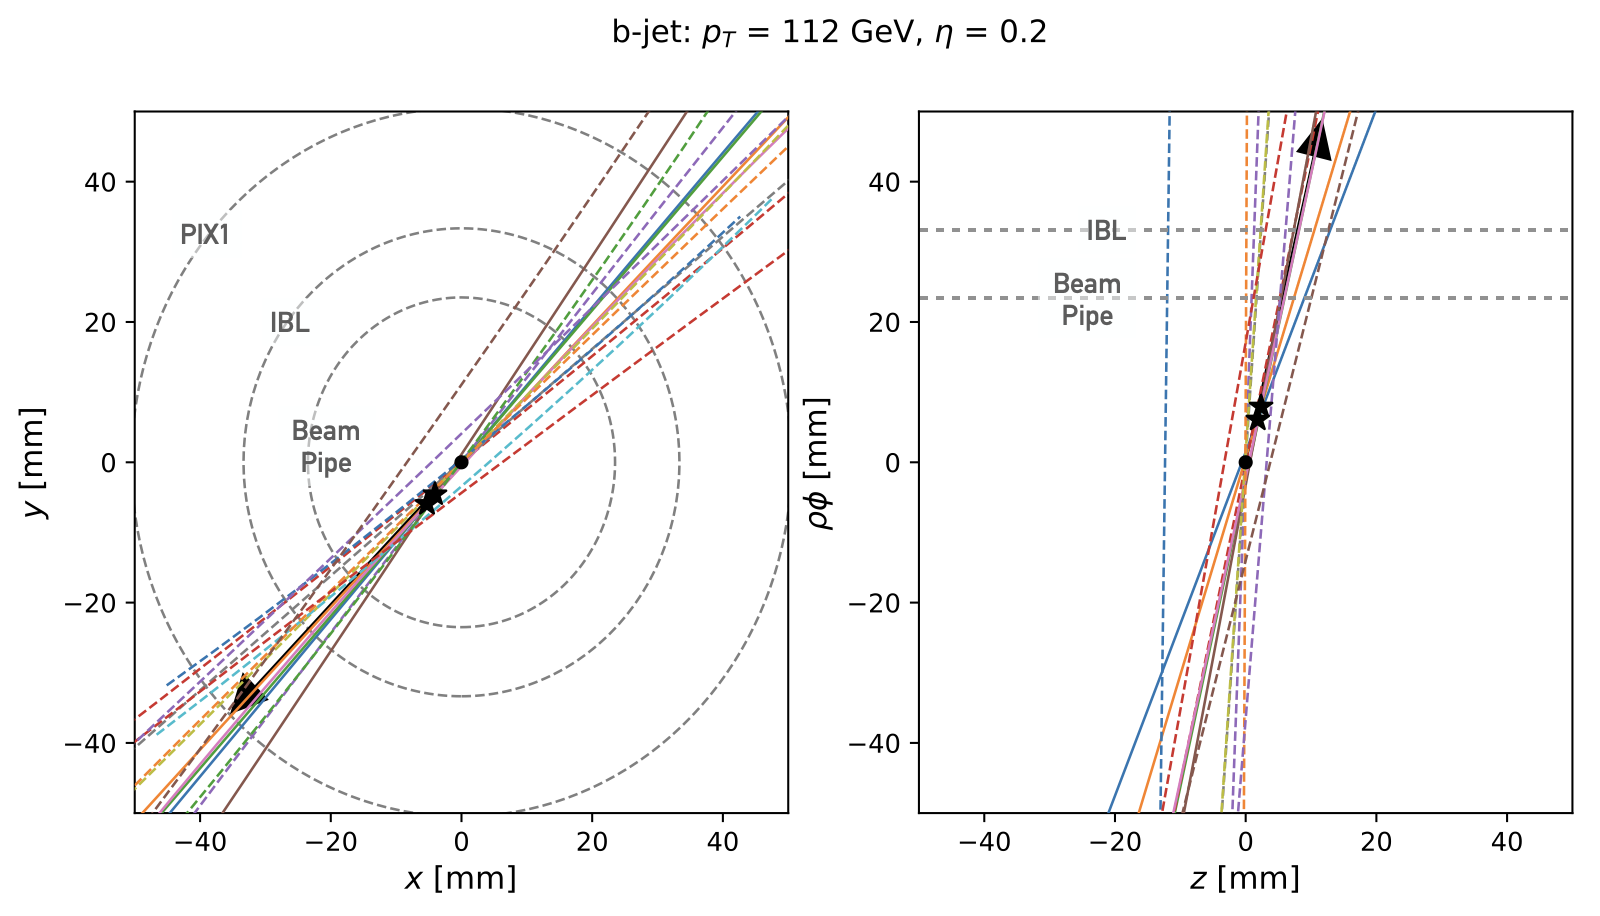
\includegraphics[height=2.75in]{{figures/ftag/jetDisplays/jet5}}
	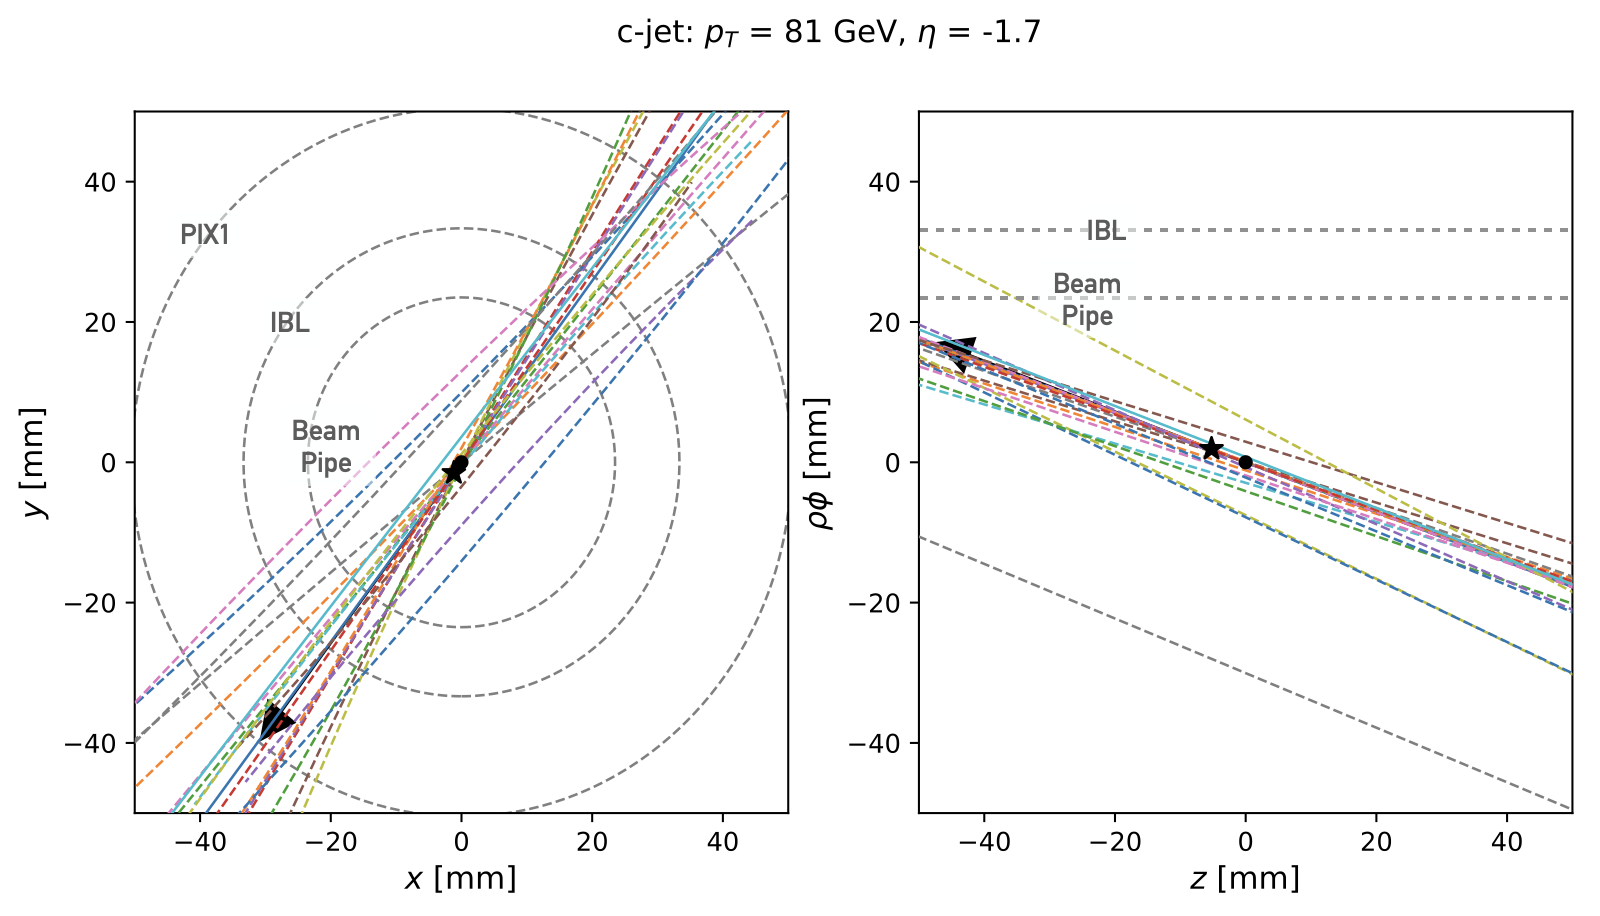
\includegraphics[height=2.75in]{{figures/ftag/jetDisplays/jet32}}
	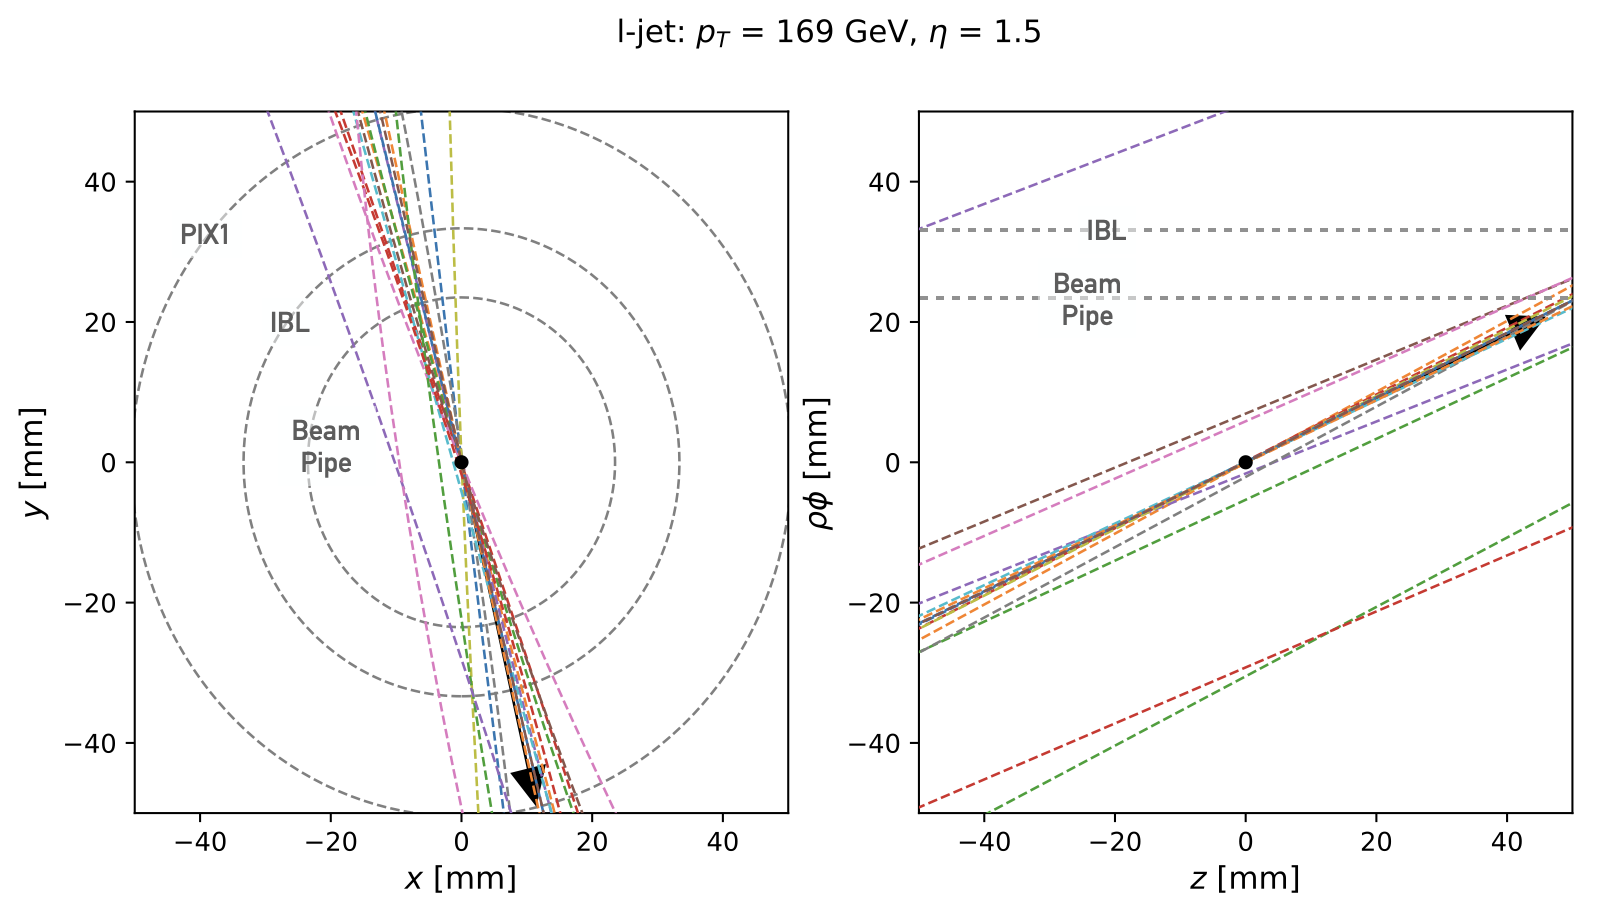
\includegraphics[height=2.75in]{{figures/ftag/jetDisplays/jet3}}
\caption{Visualization of the (x,y) and $(z,\rho\phi)$ 2d views of the tracks for reconstructing the secondary vertex (or vertices). 
The arrow on the figure indicates the jet axis, and a $\star$ shows where the weakly decaying hadron decays.
The solid lines are tracks from the HF decay, while the dashed lines denote the other tracks associated to the jet.}
\label{fig::jet-displays}
\end{figure}

\FloatBarrier
\clearpage

ATLAS employs several IP-based algorithms which are later combined with vertexing algorithms to produce a "high-level" tagger for general use.

\begin{figure}[htbp]
  \centering
  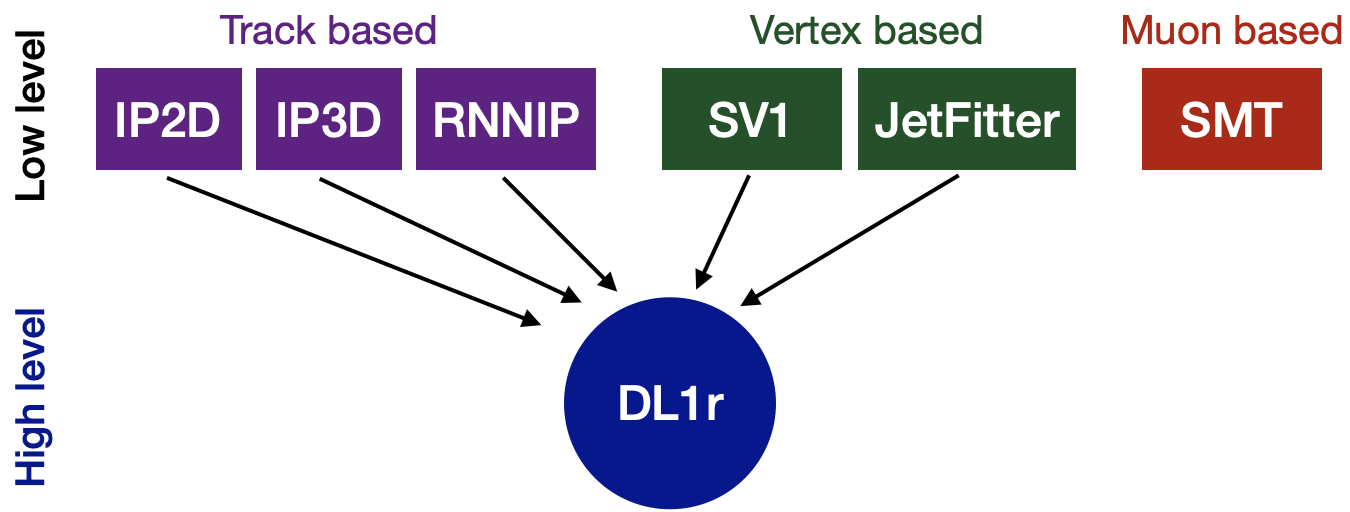
\includegraphics[width=0.9\textwidth]{figures/ftag/ATLAS-taggers}
  \caption{Types of \Pqb-taggers used on ATLAS}
  \label{fig:ATLAS-taggers}
\end{figure}

This chapter is organized as follows: Section \ref{sec:datasets} describes the datasets and selections used to train and evaluate the algorithms, while section \ref{sec:alg} details impact parameter based taggers, the Deep Sets algorithm and our specific implementation. Section \ref{sec:results} shows investigations of what the network has learned, results for the timing metrics, discussion on calibrating the algorithm, and the optimization studies conducted. Finally, section \ref{sec:conclusion} summarizes the conclusions.


\section{Datasets (?)}
\label{sec:intro}

Algorithm training and evaluation is performed with simulated $t\bar{t}$ events, produced by $\sqrt{s} = 13$~TeV proton-proton collisions, in which at least one of the W bosons, from the top quark decay, decays leptonically. 
Events are generated using the
\powhegbox~\cite{Frixione:2007nw, Nason:2004rx, Frixione:2007vw, Alioli:2010xd}~v2
generator at next-to-leading order with the NNPDF3.0NLO~\cite{Ball:2014uwa} parton set
of distribution functions~(PDF) and the \hdamp\ parameter\footnote{The
  \hdamp\ parameter is a resummation damping factor and one of the
  parameters that controls the matching of Powheg matrix elements to
  the parton shower and thus effectively regulates the
  high-\pt\ radiation against which the \ttbar\ system recoils.} set
to 1.5~\mtop~\cite{ATL-PHYS-PUB-2016-020}, with $\mtop = 172.5$ GeV.  The events are interfaced
to \pythia.230~\cite{Sjostrand:2014zea} to model the parton shower,
hadronisation, and underlying event, with parameters set according
to the A14 tune~\cite{ATL-PHYS-PUB-2014-021} and using the \nnpdftwo
set of PDFs~\cite{Ball:2012cx}. The decays of $b$ and $c$-hadrons
are performed by \evtgen~v1.6.0~\cite{Lange:2001uf}.
Particles are passed through the ATLAS detector simulation \cite{SOFT-2010-01} based on GEANT4 \cite{Agostinelli:2002hh}.

Jets are reconstructed from particle flow objects \cite{PERF-2015-09} using the anti-$k_T$ algorithm \cite{Cacciari:2008gp} with $R=0.4$. 
The jet energy scale is calibrated according to \cite{PERF-2016-04}.
Jets used for training and evaluation have $\pT \geq 20$ GeV, $|\eta|$ < 2.5, and are required not to overlap with a generator-level electron or muon from W boson decays. 
Additionally, the contamination of jets from other interactions in the beam crossing (pile-up) is surpressed by applying the jet vertex tagger \cite{ATLAS-CONF-2014-018} optimized for particle flow jets. 
%, jets with $\pT$ < 60 GeV and $|\eta|~>~2.4$ are removed if failing a jet vertex tagging (JVT) requirement that has an efficiency of 92\% for jets originating from the hard scatter vertex, with a residual rate of pile-up jets of approximately 2\%

Tracks are associated to jets using a $\Delta R$ association cone which decreases as a function of jet $\pT$, with a maximum association $\Delta R$(track, jet) of approximately 0.45 for a jet with $\pT = 20$~GeV and $\Delta R$(track, jet) of approximately 0.25 when the jet $\pT = 200$~GeV. 
If a track is within the association cones of more than one jet, it is assigned to the jet which has a smaller $\Delta R$(track, jet).

The impact parameter of the track characterises the point-of-closest approach of a track to the PV in the longitudinal ($z_0\sin \theta$) and transverse ($d_0$) planes. 
Of particular use in $b$-tagging is the IP significance defined as the impact parameter divided by its uncertainty, $s_{d0} = d_0 / \sigma_{d0}$ and $s_{z0} = z_0 \sin \theta / \sigma_{z0 \sin \theta}$. 
% The \textit{lifetime sign} is used to sign the 
The track's IP and its significance are signed according to the track's direction with respect to the jet axis and the primary vertex~\cite{PERF-2012-04}. A positive IP is expected to be consistent with a track produced from a displaced vertex. 
This procedure is referred to as lifetime signing.
%, as it aids in characterising whether the track is more likely to come from a long lived hadron or a wrongly associated tracks. \textbf{NEED LIFETIME SIGN DEFINITION}. 
The nominal track selection considered in the algorithms to be described requires tracks with $\pT  > 1$ GeV,  $|d_0| < 1$ mm, and  $|z_0 \sin \theta | < 1.5$ mm.
% We consider two track $\pT$ and IP selections for the tracks in the training. The first is the tight selection of the RNNIP algorithm with $\pT  > 1$ GeV,  $|d_0| < 1$ mm, and  $|z_0 \sin \theta | < 1.5$ mm. The second is a looser selection with $\pT$ > 500 MeV, $|d_0| <$ 3.5 mm and $|z_0 \sin \theta | <$ 5 mm.

The jets are labelled as $b$-jets if they are matched to at least one $b$-hadron having $\pT \geq 5$ GeV within $\Delta R$($b$-hadron, jet)$< 0.3$ of the jet axis. 
If this condition is not satisfied, then $c$-hadrons and then $\tau$ leptons are searched for, with similar selection criteria.
If a jet is matched to a $c$-hadron ($\tau$-lepton), it is labelled a $c$-jet ($\tau$-jet).
%,  within 0.3 of the jet axis, the jet is labelled as a $c$-jet. Jets not identified as $b$- or $c$-jets but with a $\tau$-lepton within 0.3 of the jet axis are given a $\tau$ label. 
A jet that does not meet any of these conditions is called a light-flavour jet.%, which can include jets initiated by $u$- $d$-, and $s$-quarks or gluons, although there are some residual PU jets that can leak into this category as well.

%For RNNIP, we compared training with and without a dedicated output node for jets in the $\tau$ class, but as the $\tau$ class did not improve our $b$-tagging performance, we show experiments for the network trained only on $b$, $c$, and $l$-jets.\footnote{Should I include these with and without $\tau$ node plots in the appendix?}

%textbf{Note w/ the fakes issue that Nick Style's was talking about, we will have fake tracks leaking into our fragmentation category.}


\FloatBarrier
\clearpage
\section{Low level taggers}

\subsection{IPXD}
\subsection{SV1}
\subsection{JetFitter}
\subsection{SMT}

\FloatBarrier
\clearpage
\section{Recommendations for Run 2 b-taggers}

\subsection{High level taggers: DL1 series}

We combine the low level taggers into a high-level one, the DL1r algorithm, combining information from the low-level taggers:
\begin{itemize}%[noitemsep]
	\item The IP2D and IP3D: $\log p_b$
	\item The RNNIP outputs: $p_b$, $p_c$, and $p_l$
	\item The SV1 vertex information (variables in \Tab{\ref{tab:sv1-inputs}})
	\item The JF displaced vertices characteristics, \Tab{\ref{tab:sv1-inputs}}.
\end{itemize} 


The comparisons that we'll show are again

\begin{itemize}
%\itemsep{0em}
	\item Explain architecture, optimization
	\item Explain default values
	\item pre-processing:  mean 0 and standard deviation 1 (except for the binary check variables)
\end{itemize} 

\subsection{Evaluating tagger performance}


\subsection{PFlow optimization}

\textbf{Hybrid sample definition}

In the course of the completion of this thesis, the collaboration switched from using EMTopo jets (which reconstruct a jet from the topo clusters in the calorimeter) to  using PFlow jets which cluster a jet using particle flow candidates that takes into account the better resolution of the tracker for reconstructing lower momentum objects. This improves the jet reconstruction algorithm in two ways. (1) We gain a better reconstruction of the jet \pt resolution (shown by 

\begin{itemize}
	\item Switching from EMTopo to PFlow
	\item Main improvement that we expected for $b$-tagging would be better with the better angular resolution for the jet axis
\end{itemize}

\begin{figure}[htbp]
  \centering
  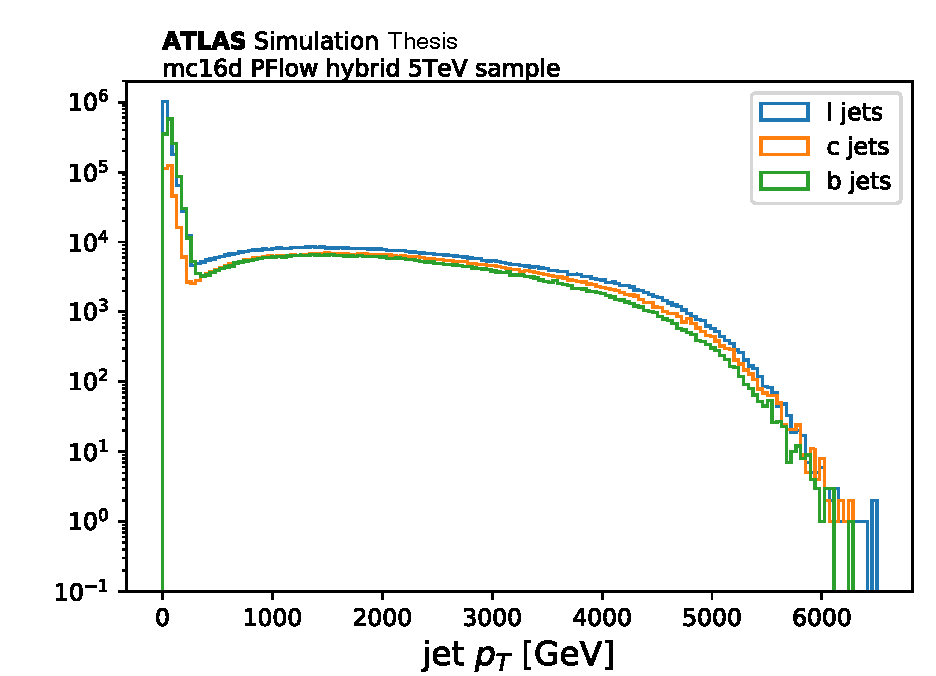
\includegraphics[width=.6\textwidth]{figures/ftag/PFlow trainings/pflow-pt-extended-hybrid}
  \caption{The \pt spectrum for training the Full Run 2 FTAG recommendations.}
  \label{fig:pflow-pt-extended-hybrid}
\end{figure}



\textbf{RNNIP optimization}

An illustration of why the task of \Pqb-tagging becomes harder at high \pt is illustrated in \Fig{\ref{fig:hf-ftag-tracks}}.


\begin{figure}[htbp]
  \centering
  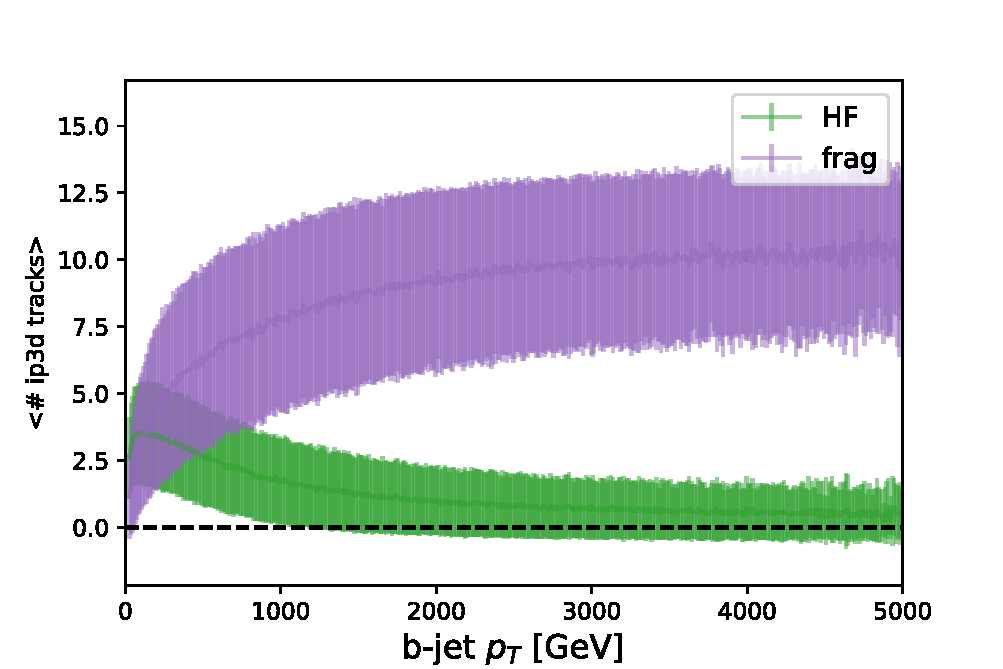
\includegraphics[width=.6\textwidth]{figures/ftag/PFlow trainings/hf-frag-tracks}
  \caption{The evolution of heavy flavor compared to the number of fragmentation tracks that have $\pt > 1~\mathrm{GeV}$, $|d_0| < 1$~mm, $|z_0 \sin \theta < 1.5$~mm, .}
  \label{fig:hf-frag-tracks}
\end{figure}


Our optimization for the RNNIP training for the PFlow tagger uses 400 hidden units in the \ldots LSTM cell.
This is an increase from the 50 hidden units of \cite{ATL-PHYS-PUB-2017-003} since training over the much larger dynamic range needed a more complex architecture.
\textbf{Do I remember what lr I used?}
The training was done with the adam optimizer, using 5 million jets, and 20\% of the dataset was held out as a validation set, and the training was stopped when the validation loss had not improved in the last 20 epochs.


\begin{figure}
\centering
\subfloat[light rejection]{
	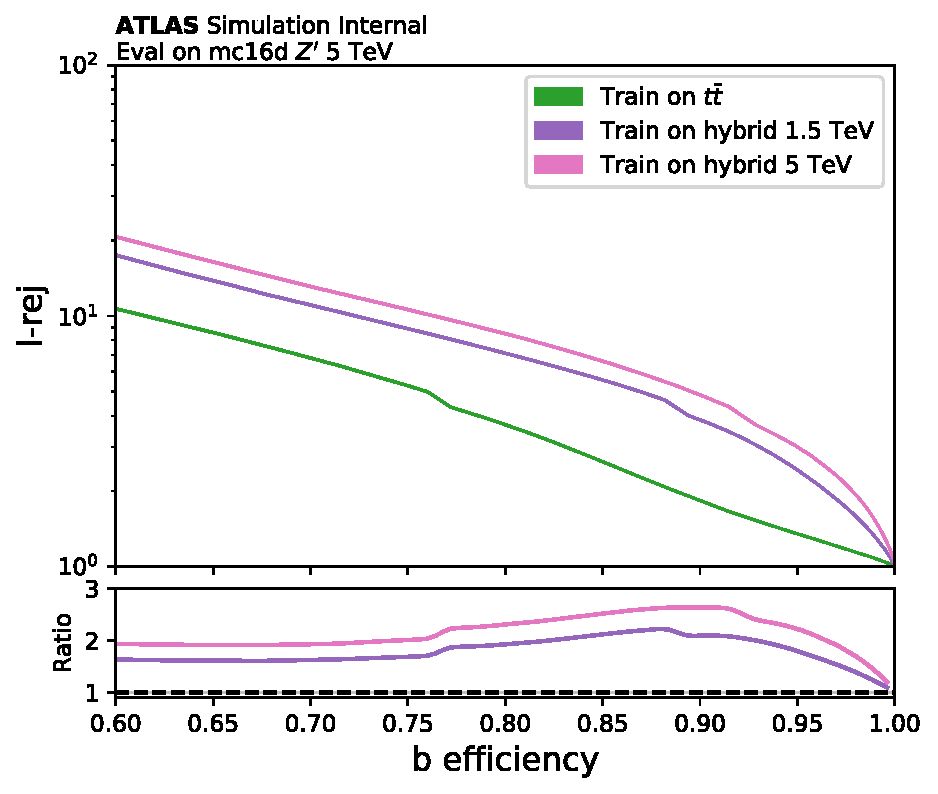
\includegraphics[width=0.45\textwidth]{{figures/ftag/PFlow\ Trainings/Zprime-l-roc}}
	}
\subfloat[\Pqc rejection]{
	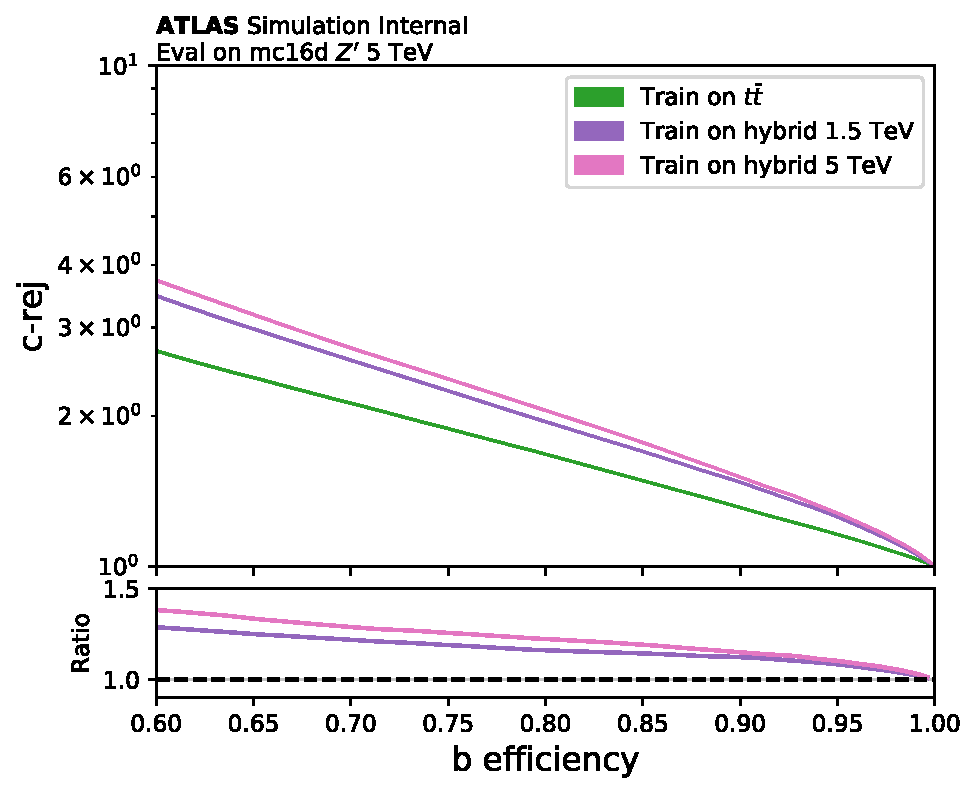
\includegraphics[width=0.45\textwidth]{{figures/ftag/PFlow\ Trainings/Zprime-c-roc}}
	}
\caption{}
\label{fig:Zprime-c-roc}
\end{figure}


\begin{figure}
\centering
\subfloat[light rejection]{
	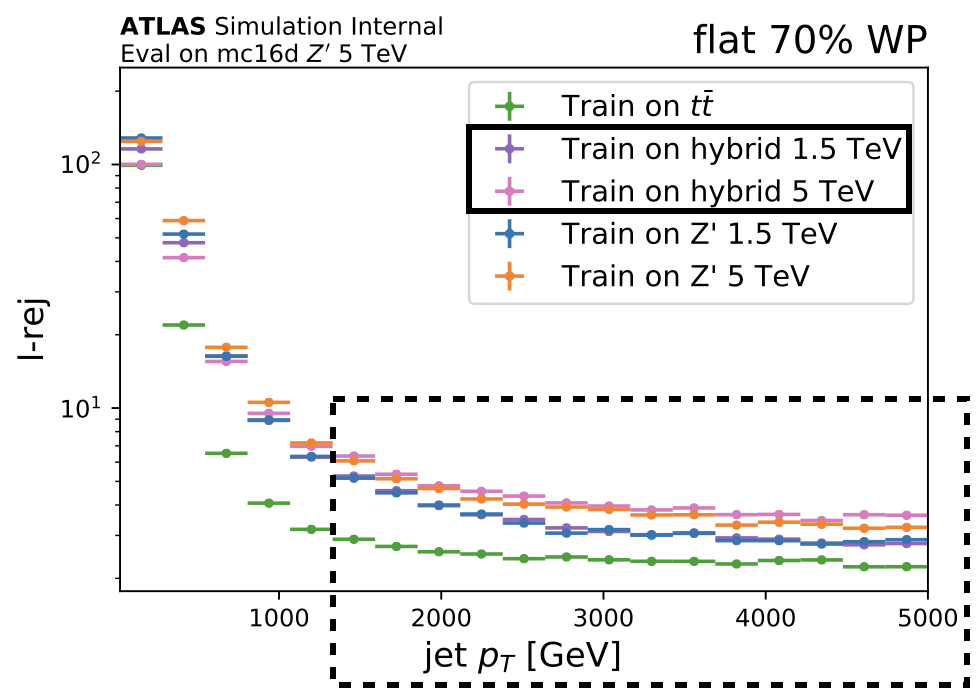
\includegraphics[width=0.45\textwidth]{{figures/ftag/PFlow\ Trainings/Zprime-l-pt}}
	}
\subfloat[\Pqc rejection]{
	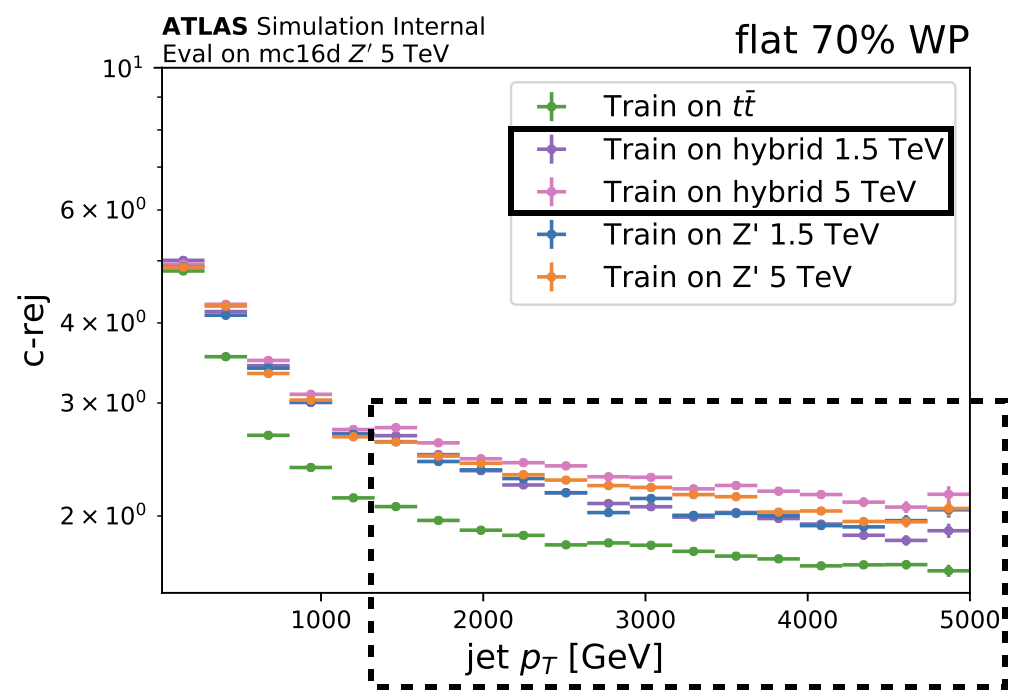
\includegraphics[width=0.45\textwidth]{{figures/ftag/PFlow\ Trainings/Zprime-c-pt}}
	}
\caption{}
\label{fig:Zprime-pt}
\end{figure}



\begin{figure}
\centering
\subfloat[light rejection]{
	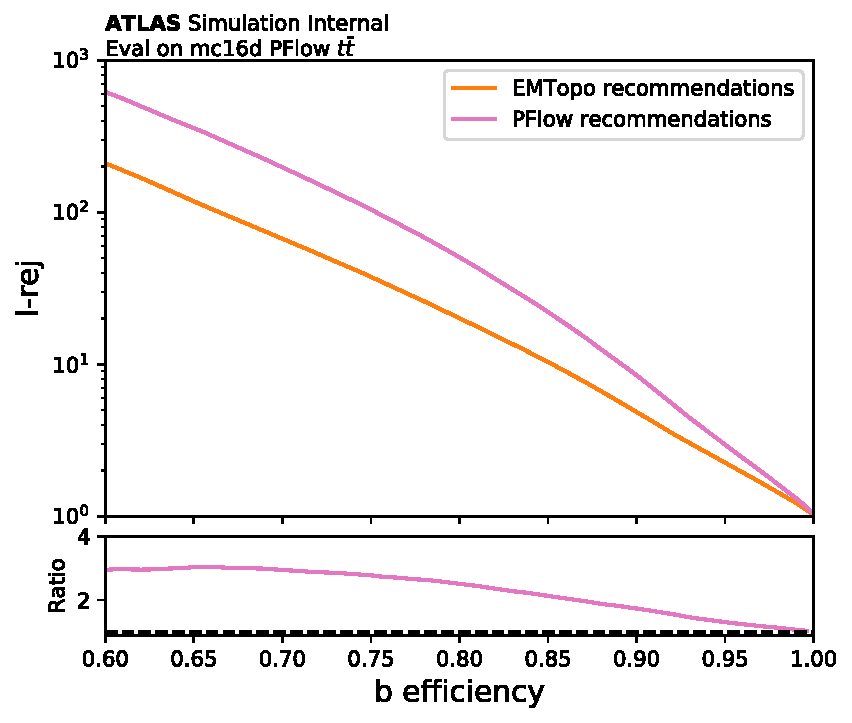
\includegraphics[width=0.45\textwidth]{{figures/ftag/PFlow\ Trainings/topo-vs-pflow-l-rej}}
	}
\subfloat[\Pqc rejection]{
	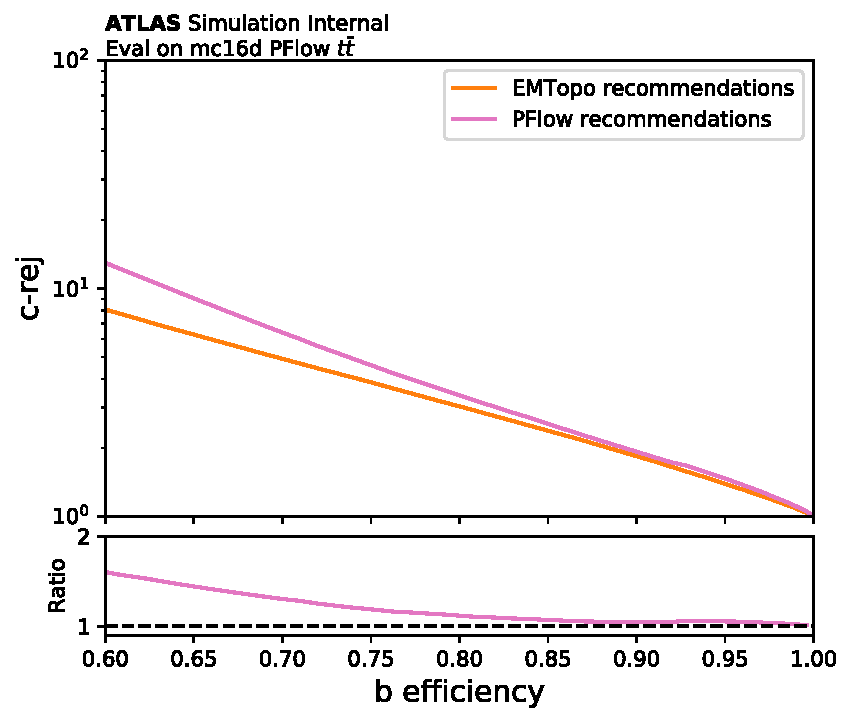
\includegraphics[width=0.45\textwidth]{{figures/ftag/PFlow\ Trainings/topo-vs-pflow-c-rej}}
	}
\caption{}
\label{fig:topo-pflow}
\end{figure}

The EMTopo training recommendation was from the 2017 retraining campaign:

Rafael showed we see retraining gains due to the kinematics changes with hdamp from mc15 -> mc16

Dedicated retraining on new pflow jet collection

Plus the RNN improvements from this year




\textbf{DL1r results}


% PFlow results link
% http://atlas.web.cern.ch/Atlas/GROUPS/PHYSICS/PLOTS/FTAG-2019-005/
\def\jetdef{PFlow}
\def\figpath{figures/ftag/\jetdef \ trainings}

\begin{figure}[htbp]
    \centering
    % light
    \subfloat[]{ 
            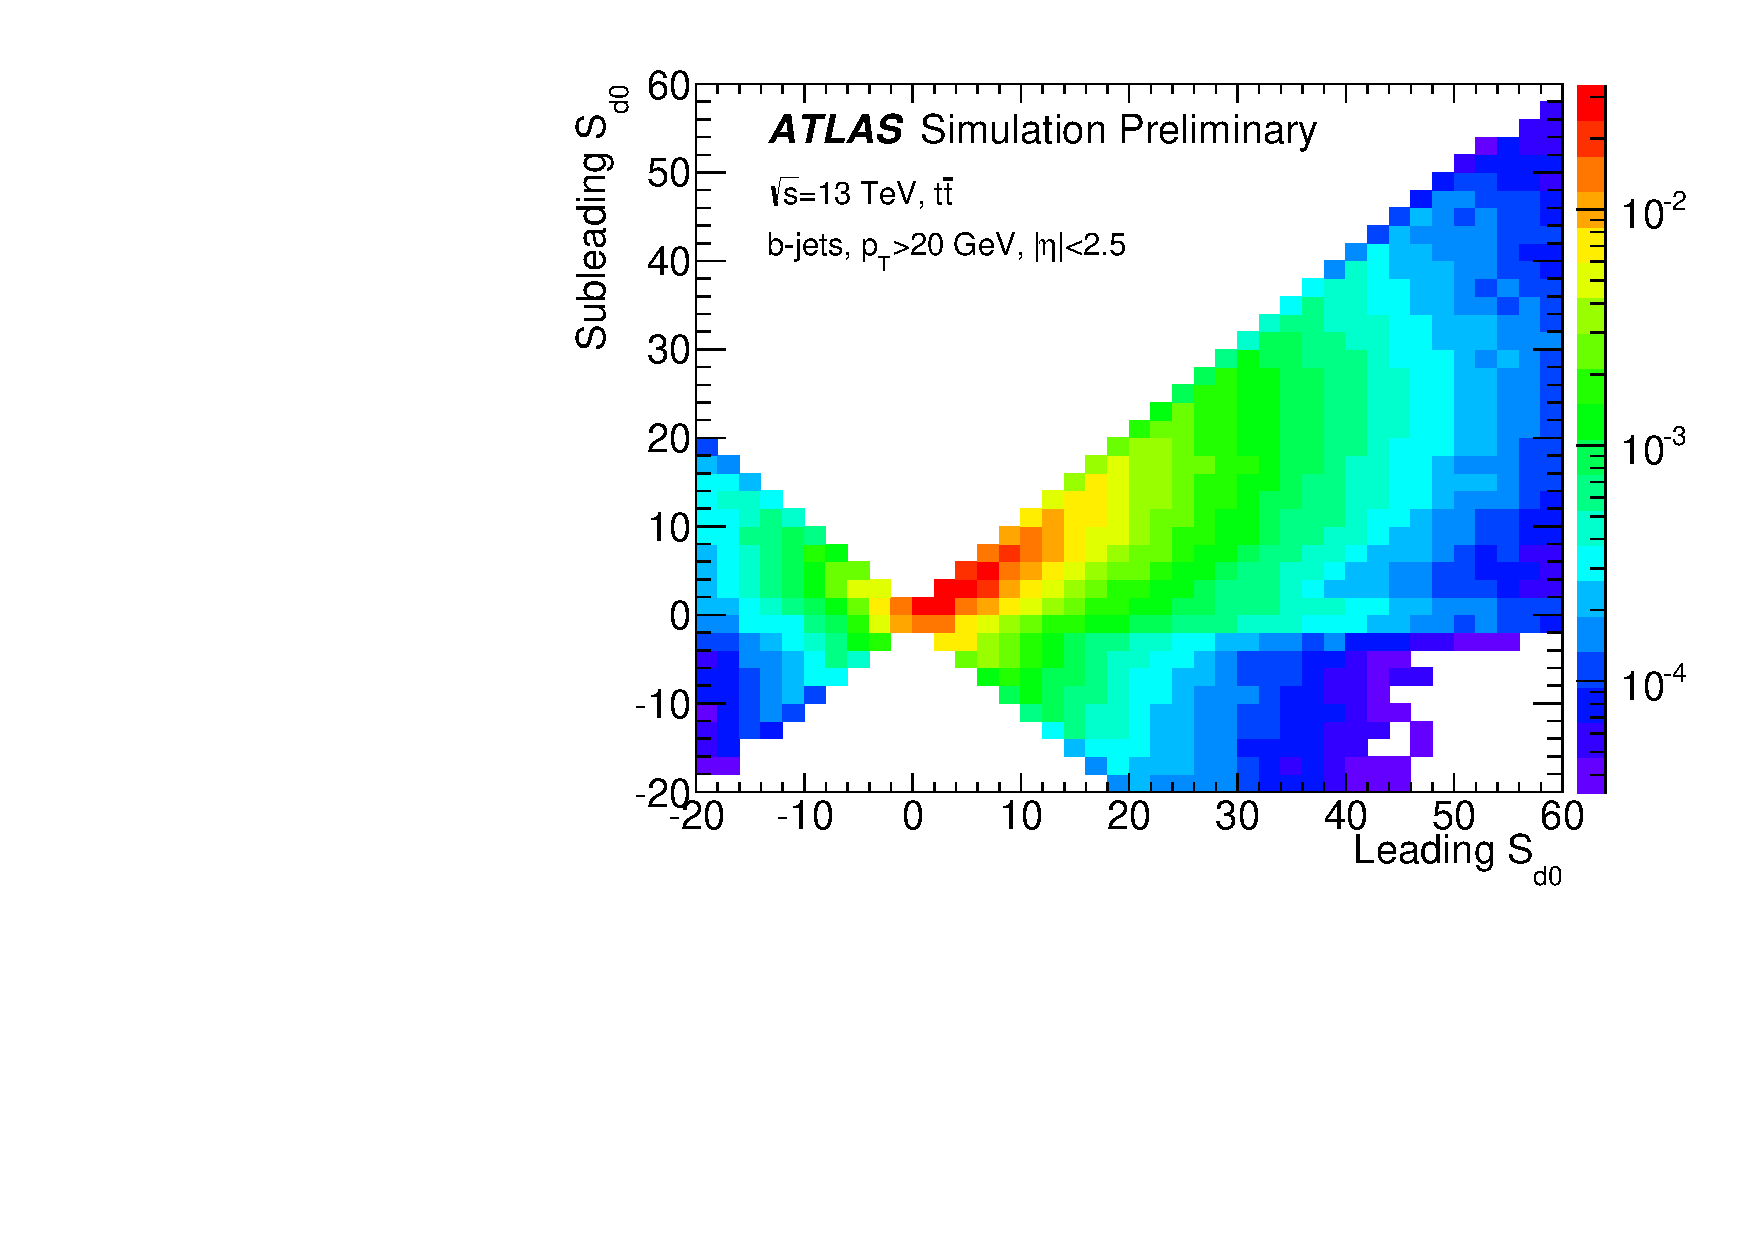
\includegraphics[width=0.48\linewidth]{\figpath/fig_01a}
    } 
     \subfloat[]{ 
            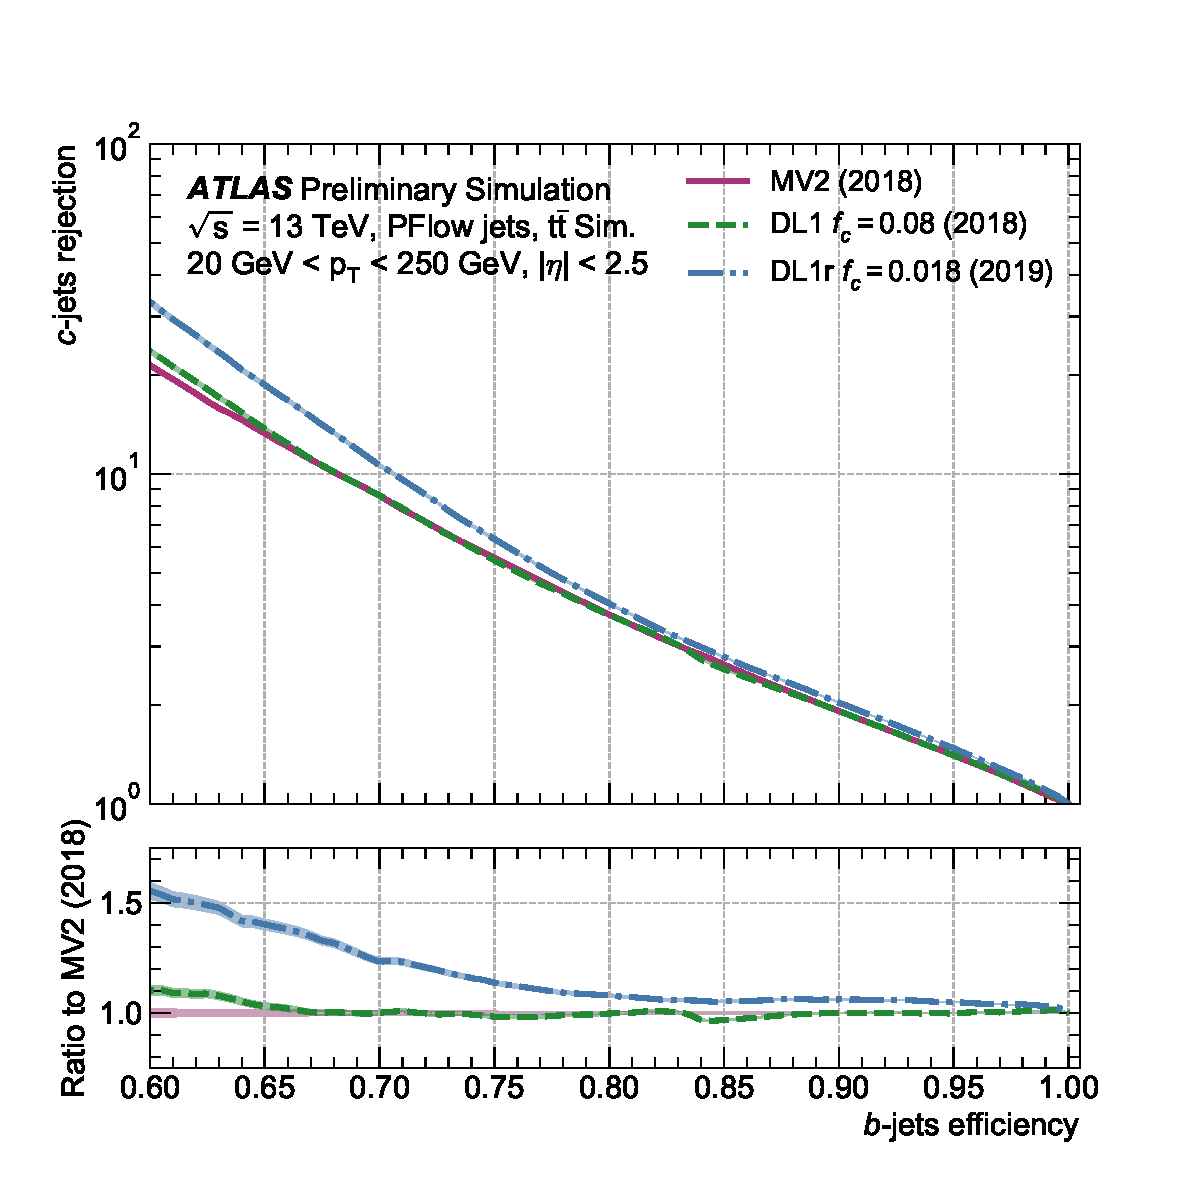
\includegraphics[width=0.48\linewidth]{\figpath/fig_01b}
    } 
    \caption{}
    \label{fig:\jetdef-fig1}
\end{figure}

\begin{figure}[htbp]
    \centering
    % light
    \subfloat[]{ 
            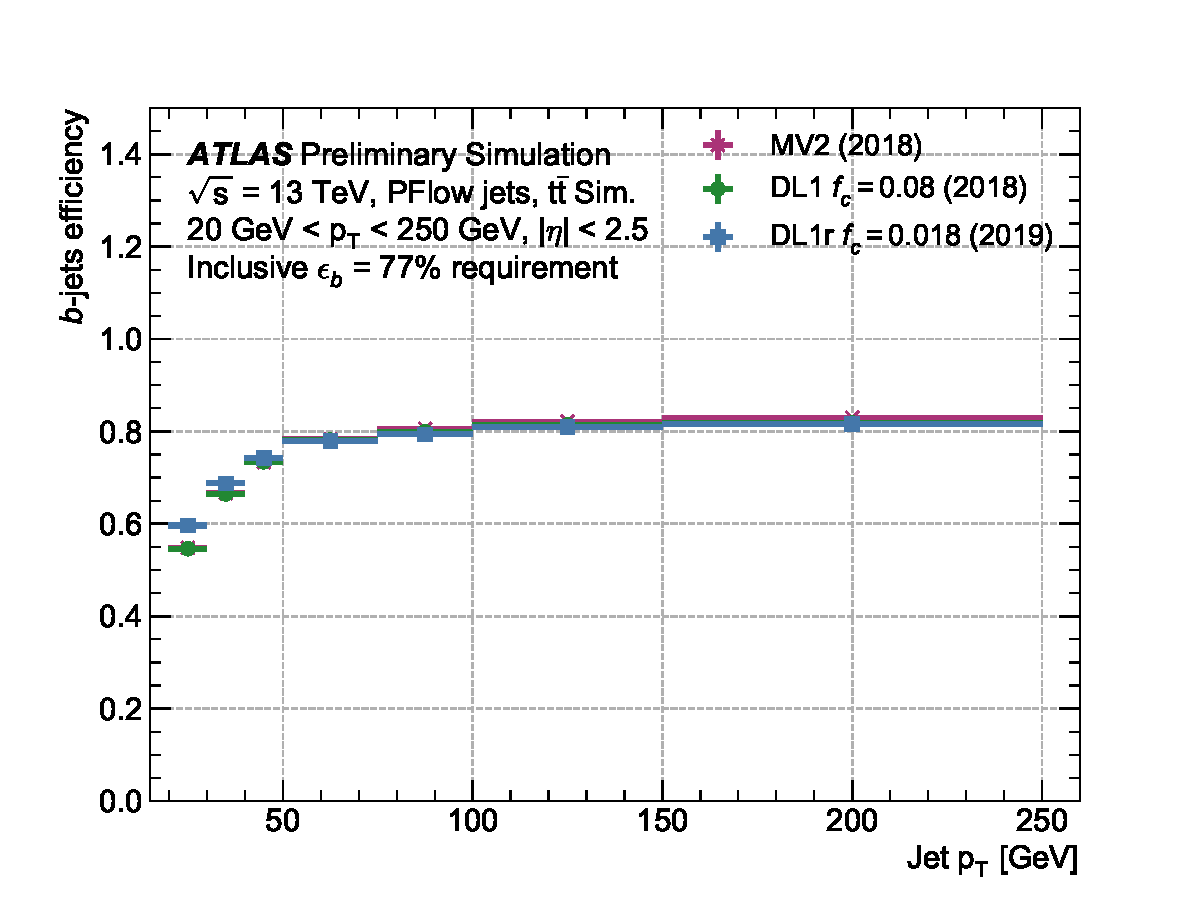
\includegraphics[width=0.33\linewidth]{\figpath/fig_02a}
    } 
     \subfloat[]{ 
            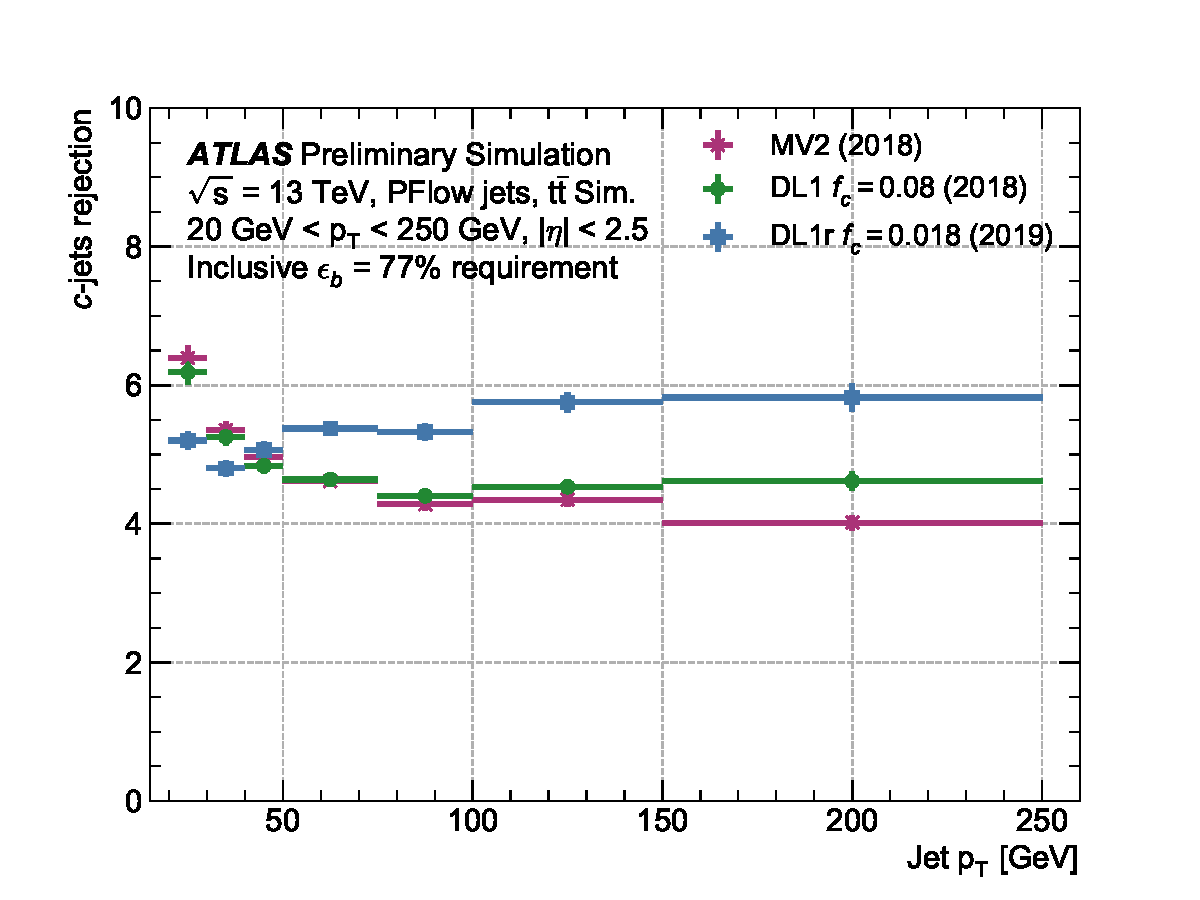
\includegraphics[width=0.33\linewidth]{\figpath/fig_02b}
    } 
    \subfloat[]{ 
            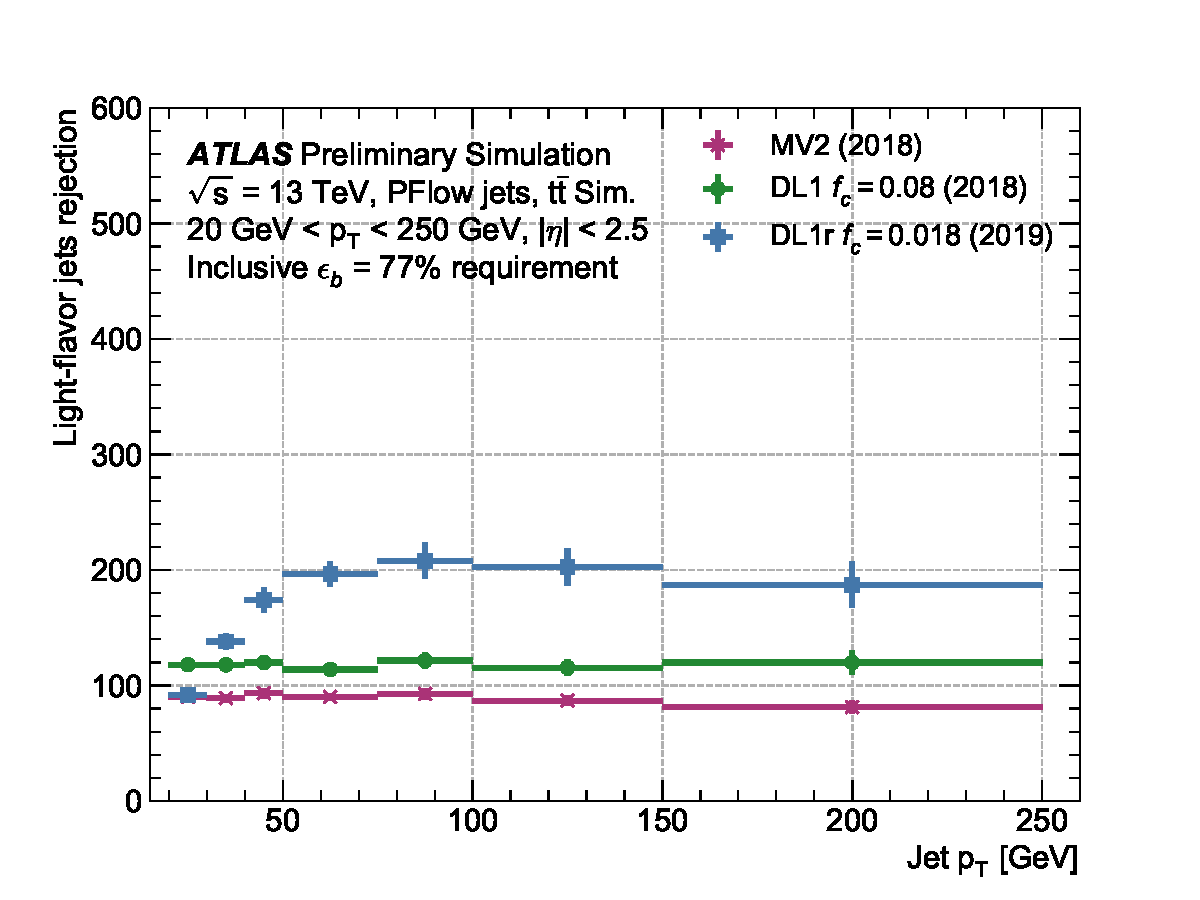
\includegraphics[width=0.33\linewidth]{\figpath/fig_02c}
    } 
    \caption{}
    \label{fig:\jetdef-fig2}
\end{figure}

\begin{figure}[htbp]
    \centering
    % light
    \subfloat[]{ 
            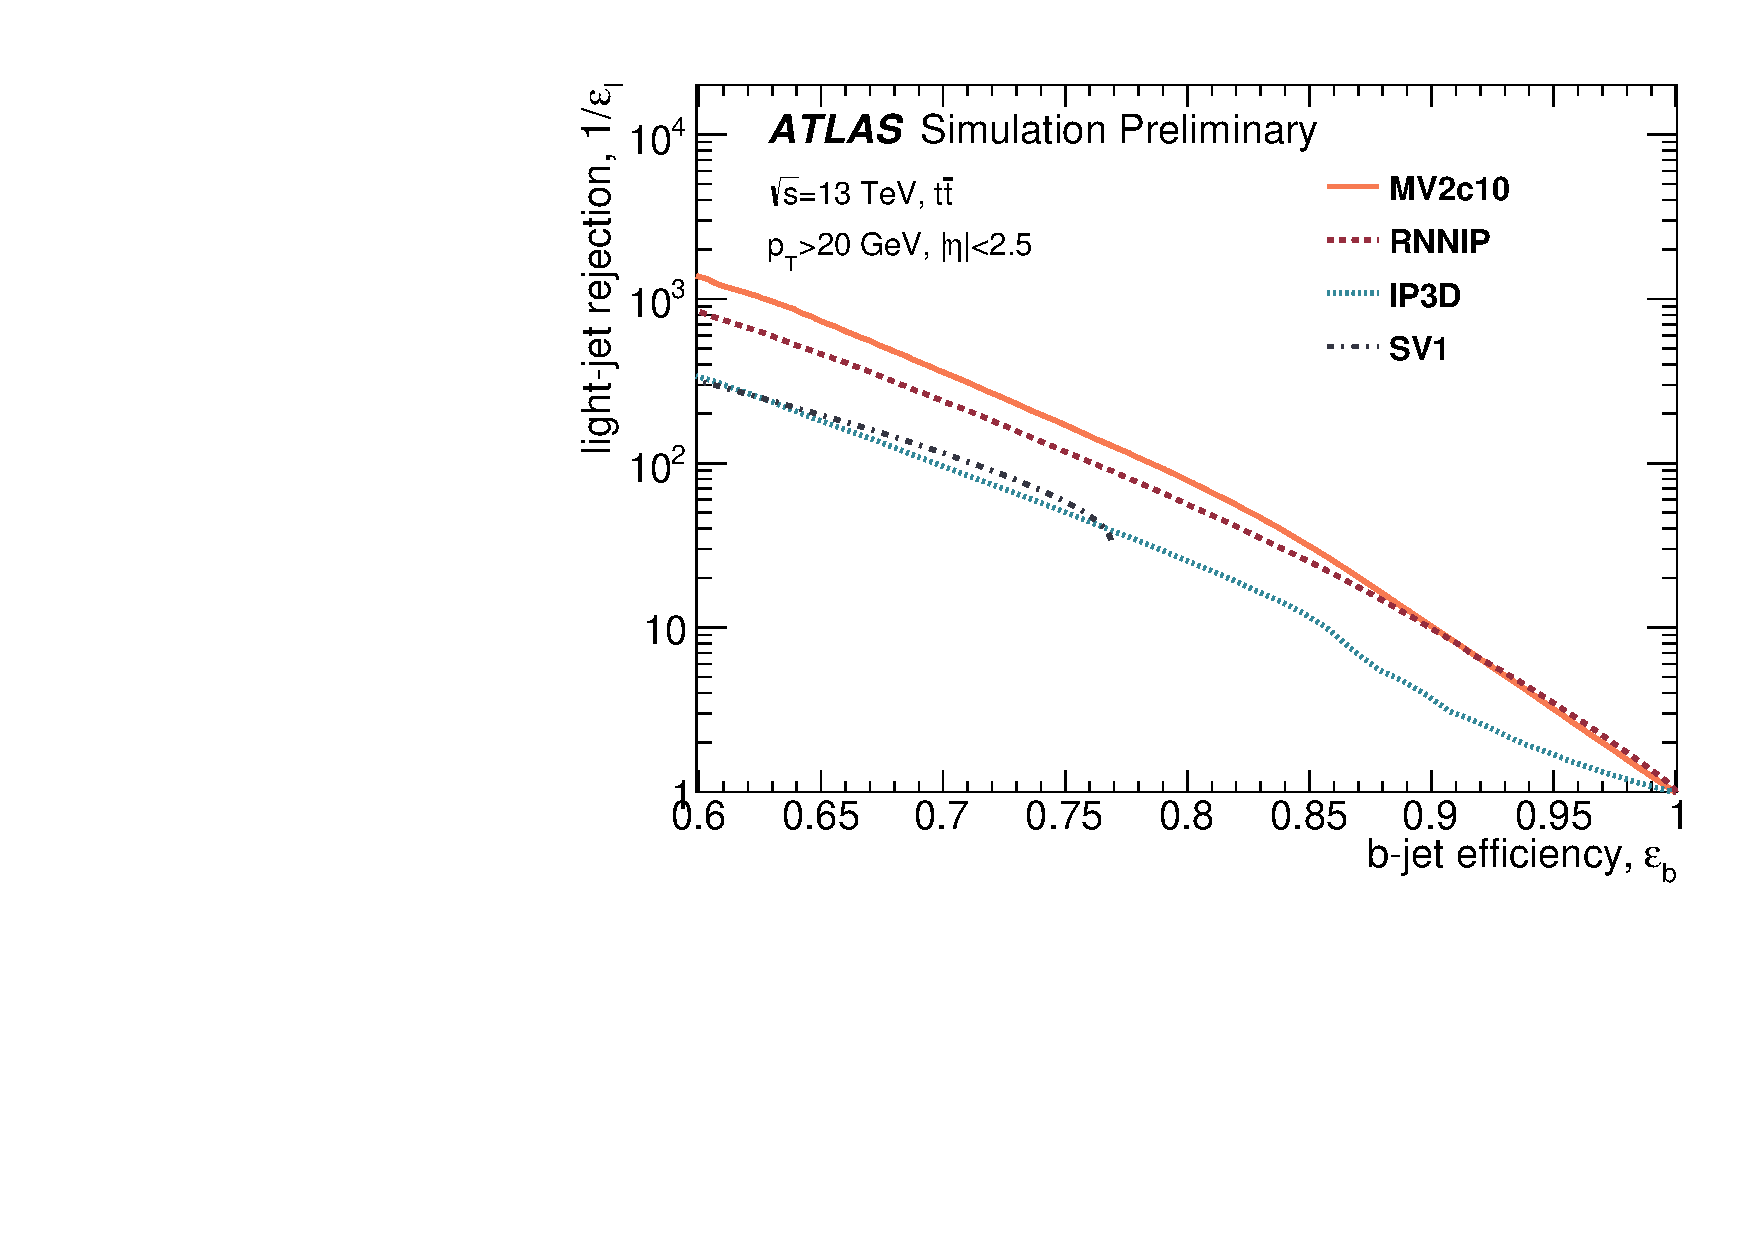
\includegraphics[width=0.48\linewidth]{\figpath/fig_03a}
    } 
     \subfloat[]{ 
            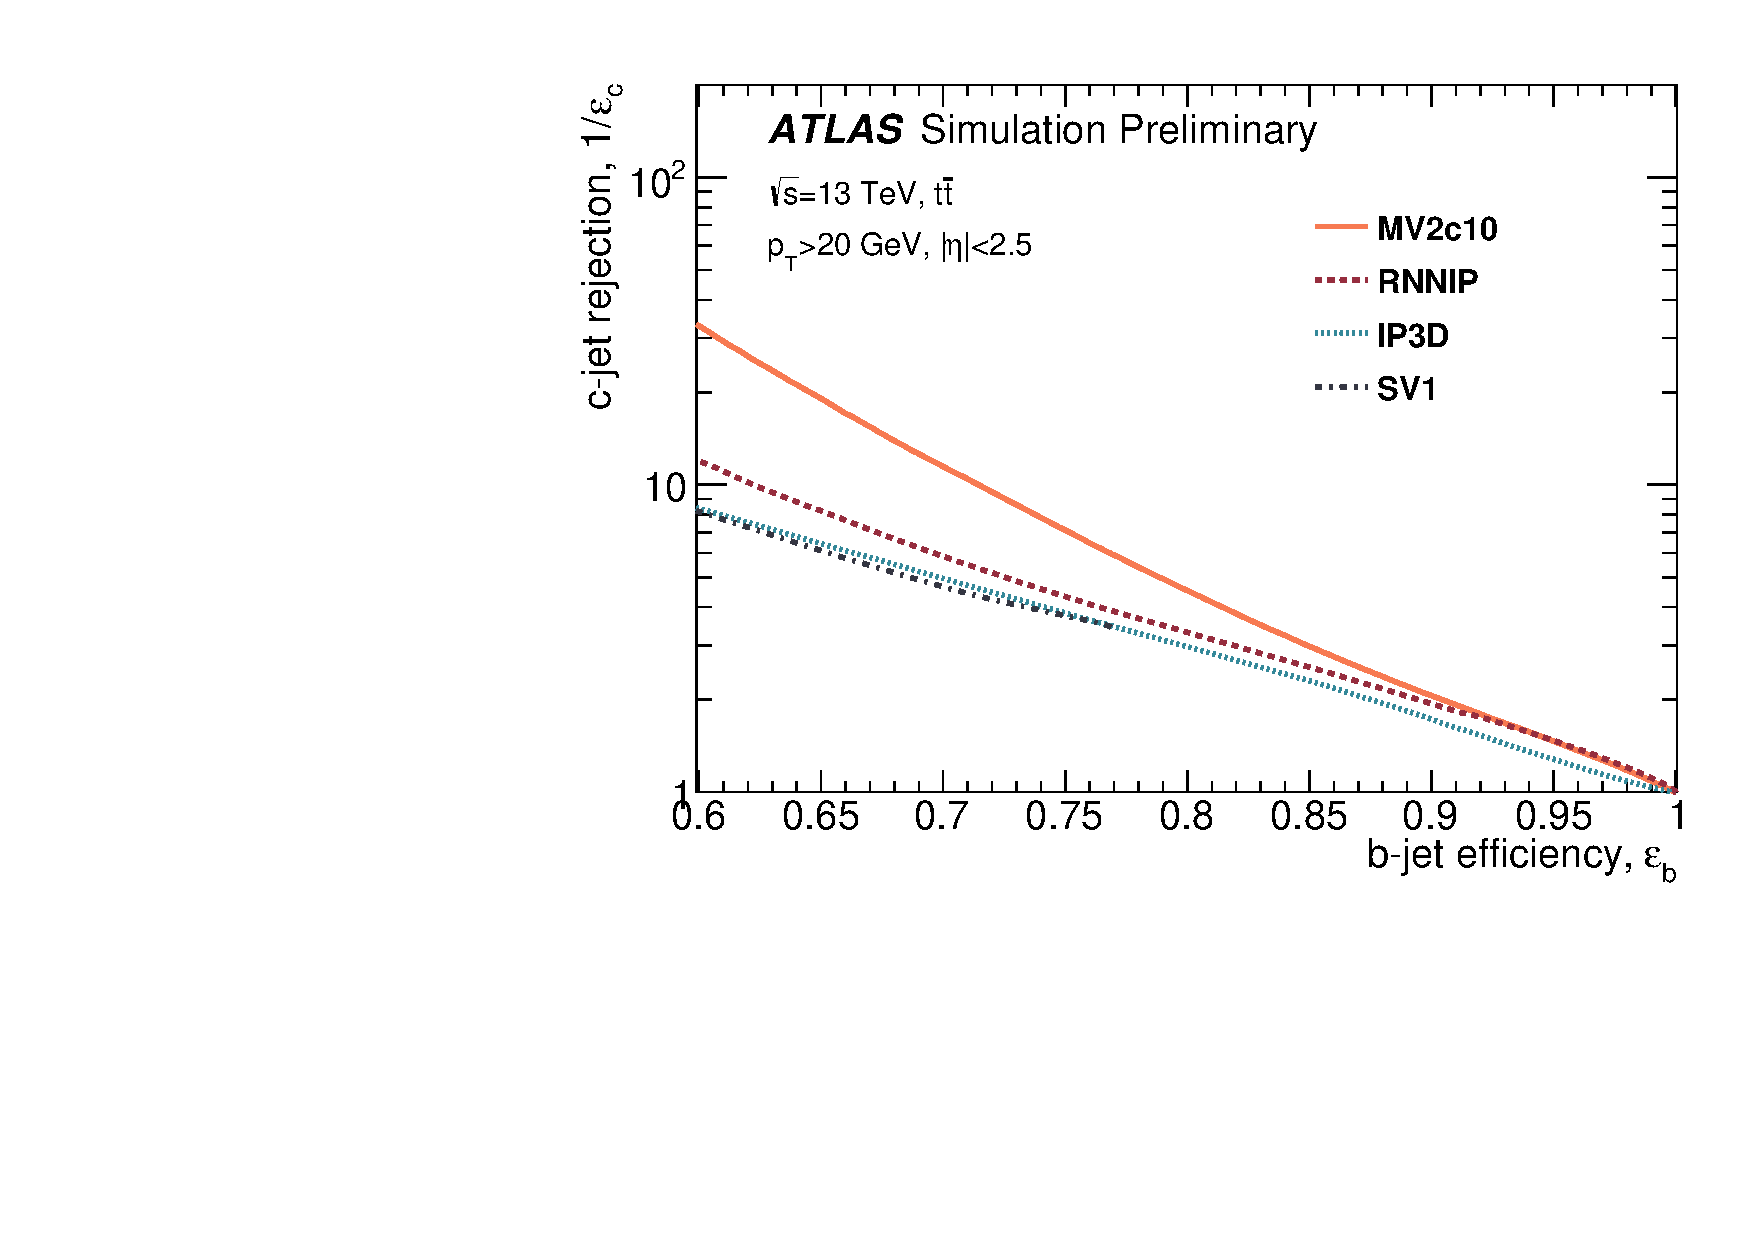
\includegraphics[width=0.48\linewidth]{\figpath/fig_03b}
    } 
    \caption{}
    \label{fig:\jetdef-fig3}
\end{figure}





%%%%%%%%%%%%%%%%%%%%%%%%%%%%%%
% VR track jets
%%%%%%%%%%%%%%%%%%%%%%%%%%%%%%

\FloatBarrier
\clearpage
\subsection{VR track jets optimization}

\hl{I had to have had a dR matching in this plot \ldots let's look up what it was!}

\begin{figure}[htbp]
  \centering
  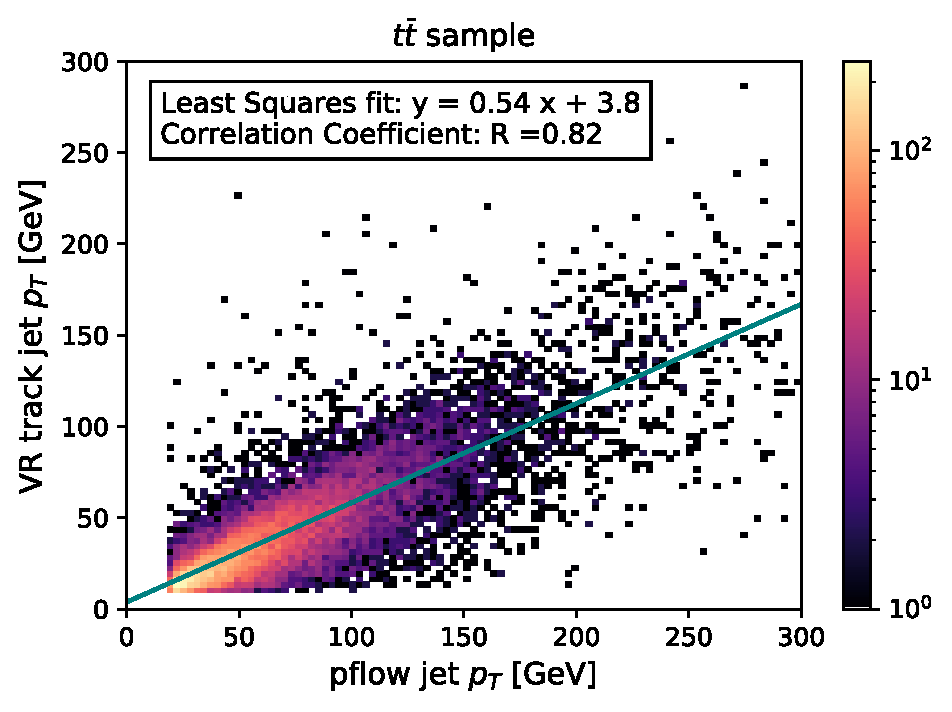
\includegraphics[width=.45\textwidth]{figures/ftag/VR trainings/pt-VR-pflow-ttvar}
  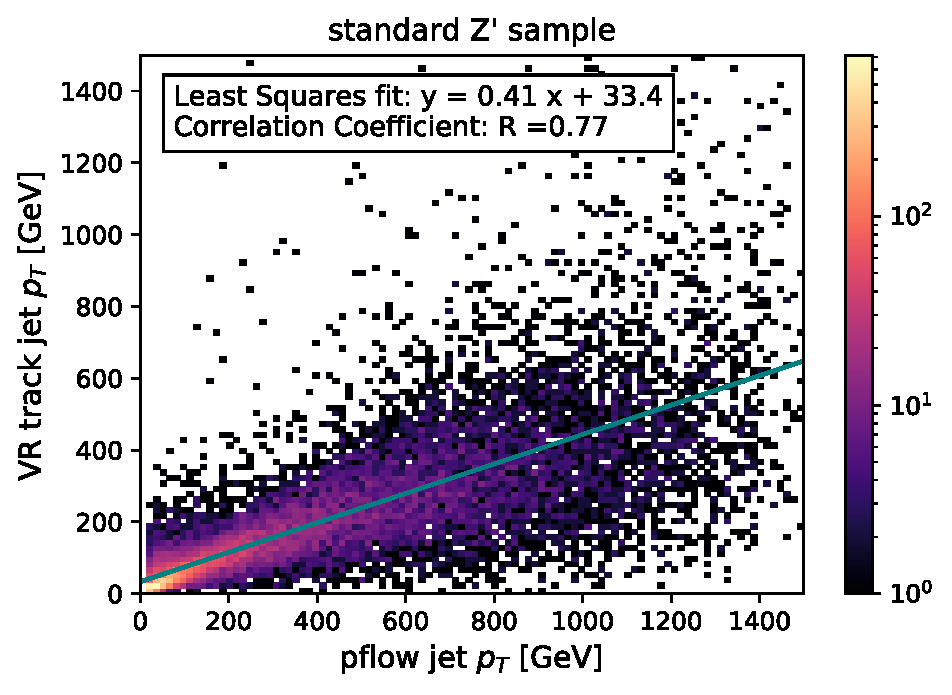
\includegraphics[width=.45\textwidth]{figures/ftag/VR trainings/pt-VR-pflow-std-Zprime}
  \caption{Comparison of the PFlow and VR track jet \pt for jet reconstruction.}
  \label{fig:pt-VR-pflow}
\end{figure}

Note: This plot \emph{motivated} us to move the pT cut on the light and c-jets to 125~GeV (although we kept the b-hadron \pt cut at 250 GeV).

\begin{figure}[htbp]
  \centering
  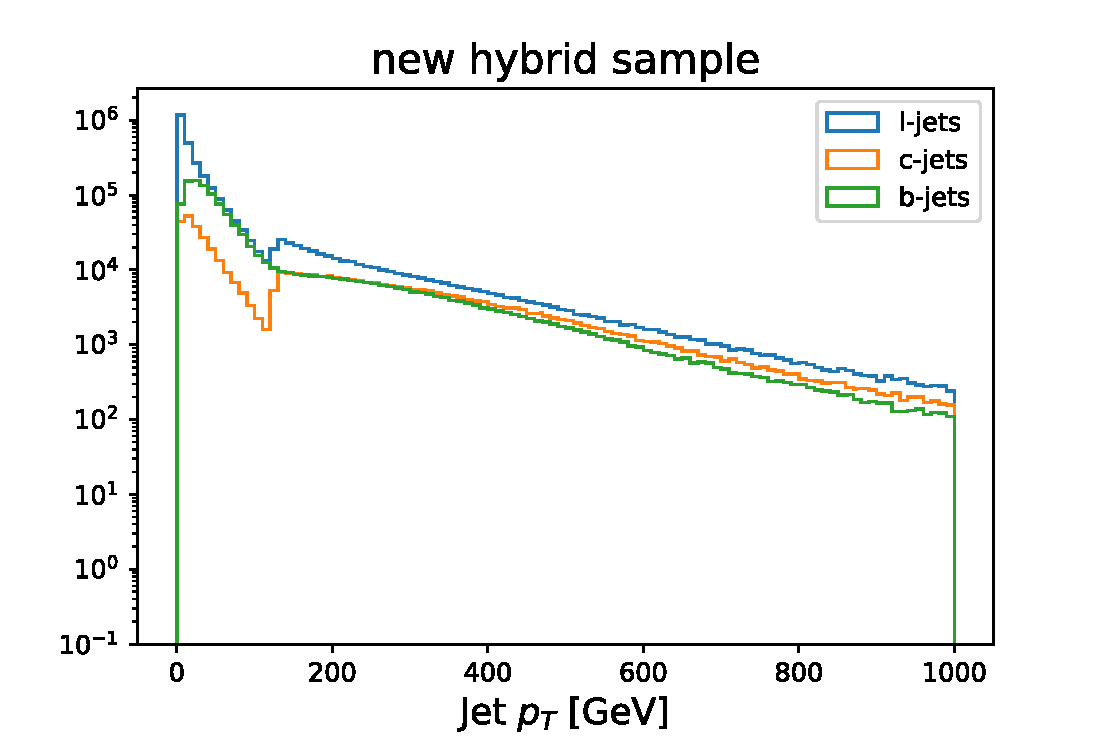
\includegraphics[width=.6\textwidth]{figures/ftag/VR trainings/pt-hyb-vr}
  \caption{The \pt spectrum for the VR track jets using the modified sample cut of 125~GeV for the light jet and \Pqb-jet \pt.}
  \label{fig:pflow-pt-extended-hybrid}
\end{figure}



\begin{figure}
\centering
\subfloat[light rejection]{
	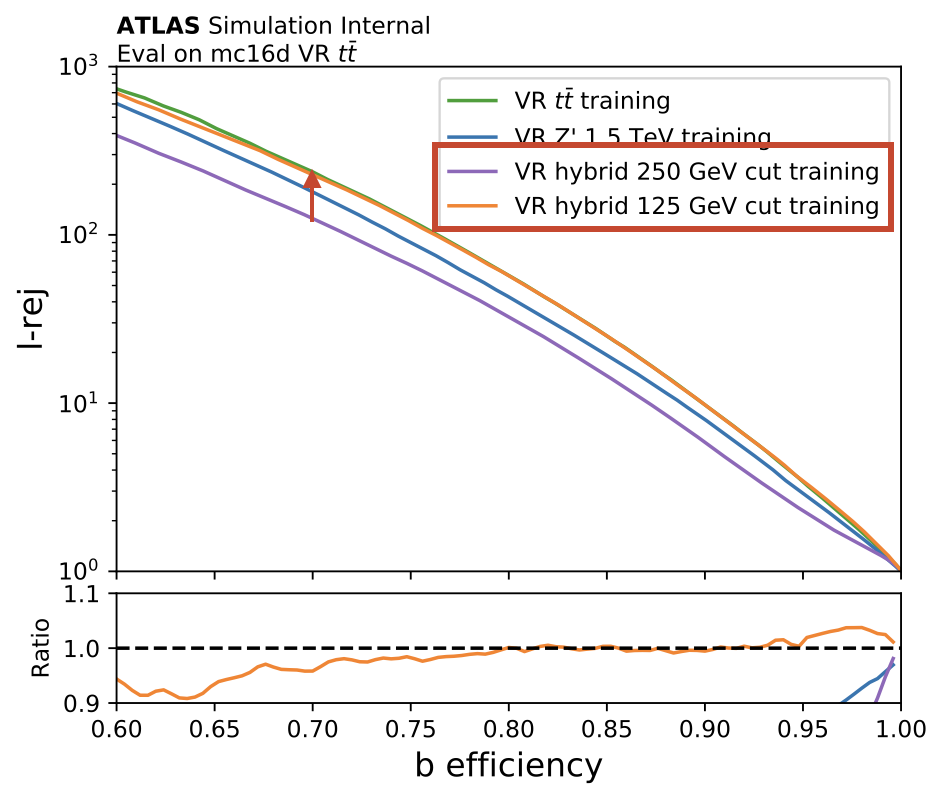
\includegraphics[width=0.45\textwidth]{{figures/ftag/VR\ Trainings/roc-new-cut-l-ttbar}}
	}
\subfloat[\Pqc rejection]{
	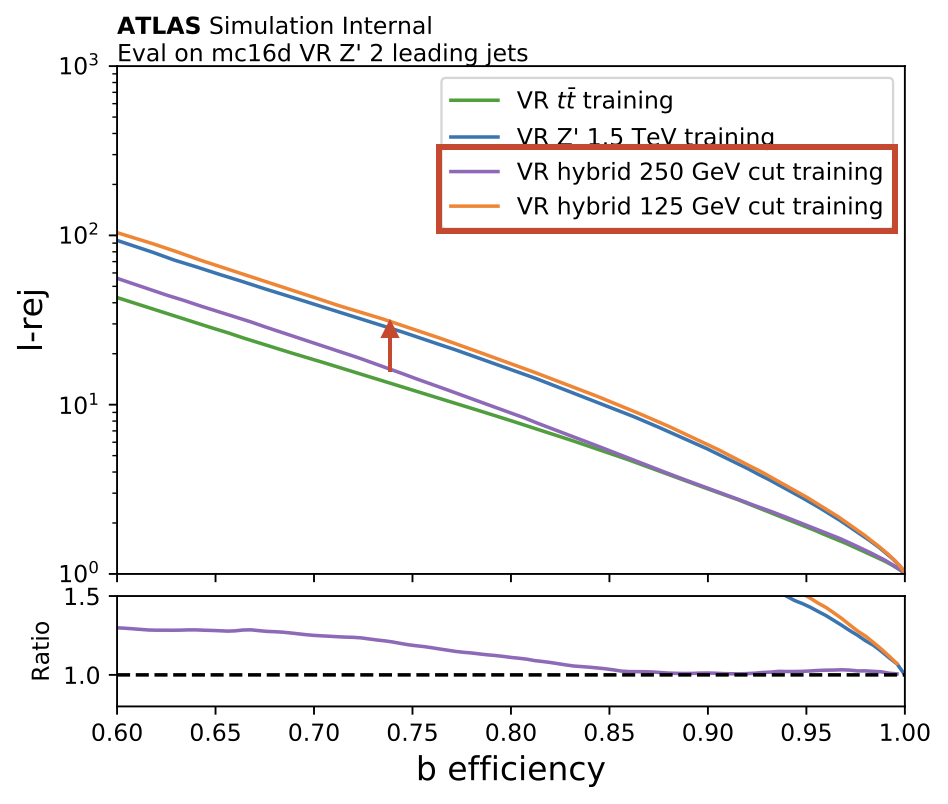
\includegraphics[width=0.45\textwidth]{{figures/ftag/VR\ Trainings/roc-new-cut-l-Zprime}}
	}
\caption{}
\label{fig:VR-improvements}
\end{figure}



\begin{figure}
\centering
\subfloat[light rejection]{
	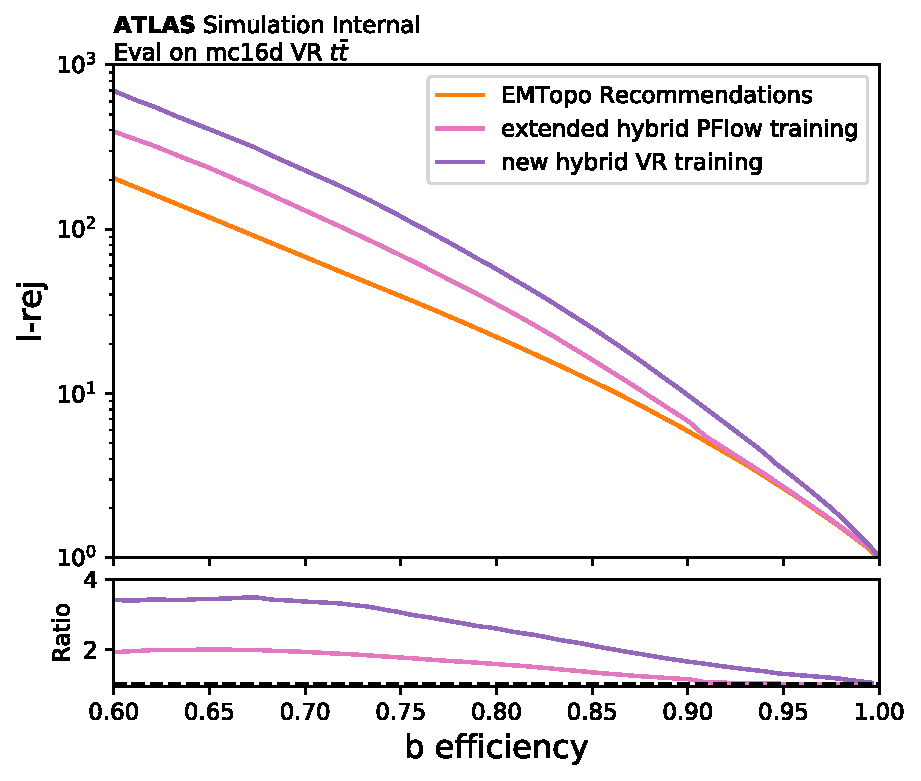
\includegraphics[width=0.45\textwidth]{{figures/ftag/VR\ Trainings/roc-vr-trainings-l}}
	}
\subfloat[\Pqc rejection]{
	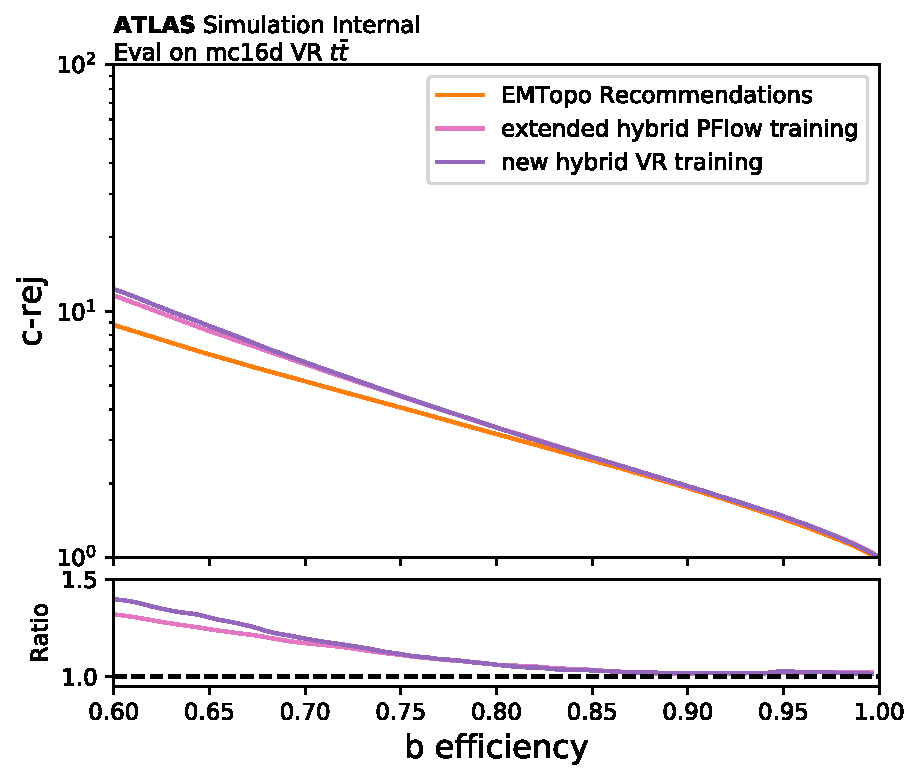
\includegraphics[width=0.45\textwidth]{{figures/ftag/VR\ Trainings/roc-vr-trainings-c}}
	}
\caption{}
\label{fig:VR-improvements}
\end{figure}

\begin{enumerate}
	\item \textcolor{orange}{EMTopo Rec: What we were applying to VR track jets now}
	\item \textcolor{deeppink}{Ext Pflow: If we applied the my new pflow training to VR track jets}
	\item \textcolor{mediumpurple}{New hybrid VR training: NEW dedicated VR training}
\end{enumerate}




\def\jetdef{VR}
% http://atlas.web.cern.ch/Atlas/GROUPS/PHYSICS/PLOTS/FTAG-2019-006/

\def\figpath{figures/ftag/\jetdef \ trainings}

\begin{figure}[htbp]
    \centering
    % light
    \subfloat[]{ 
            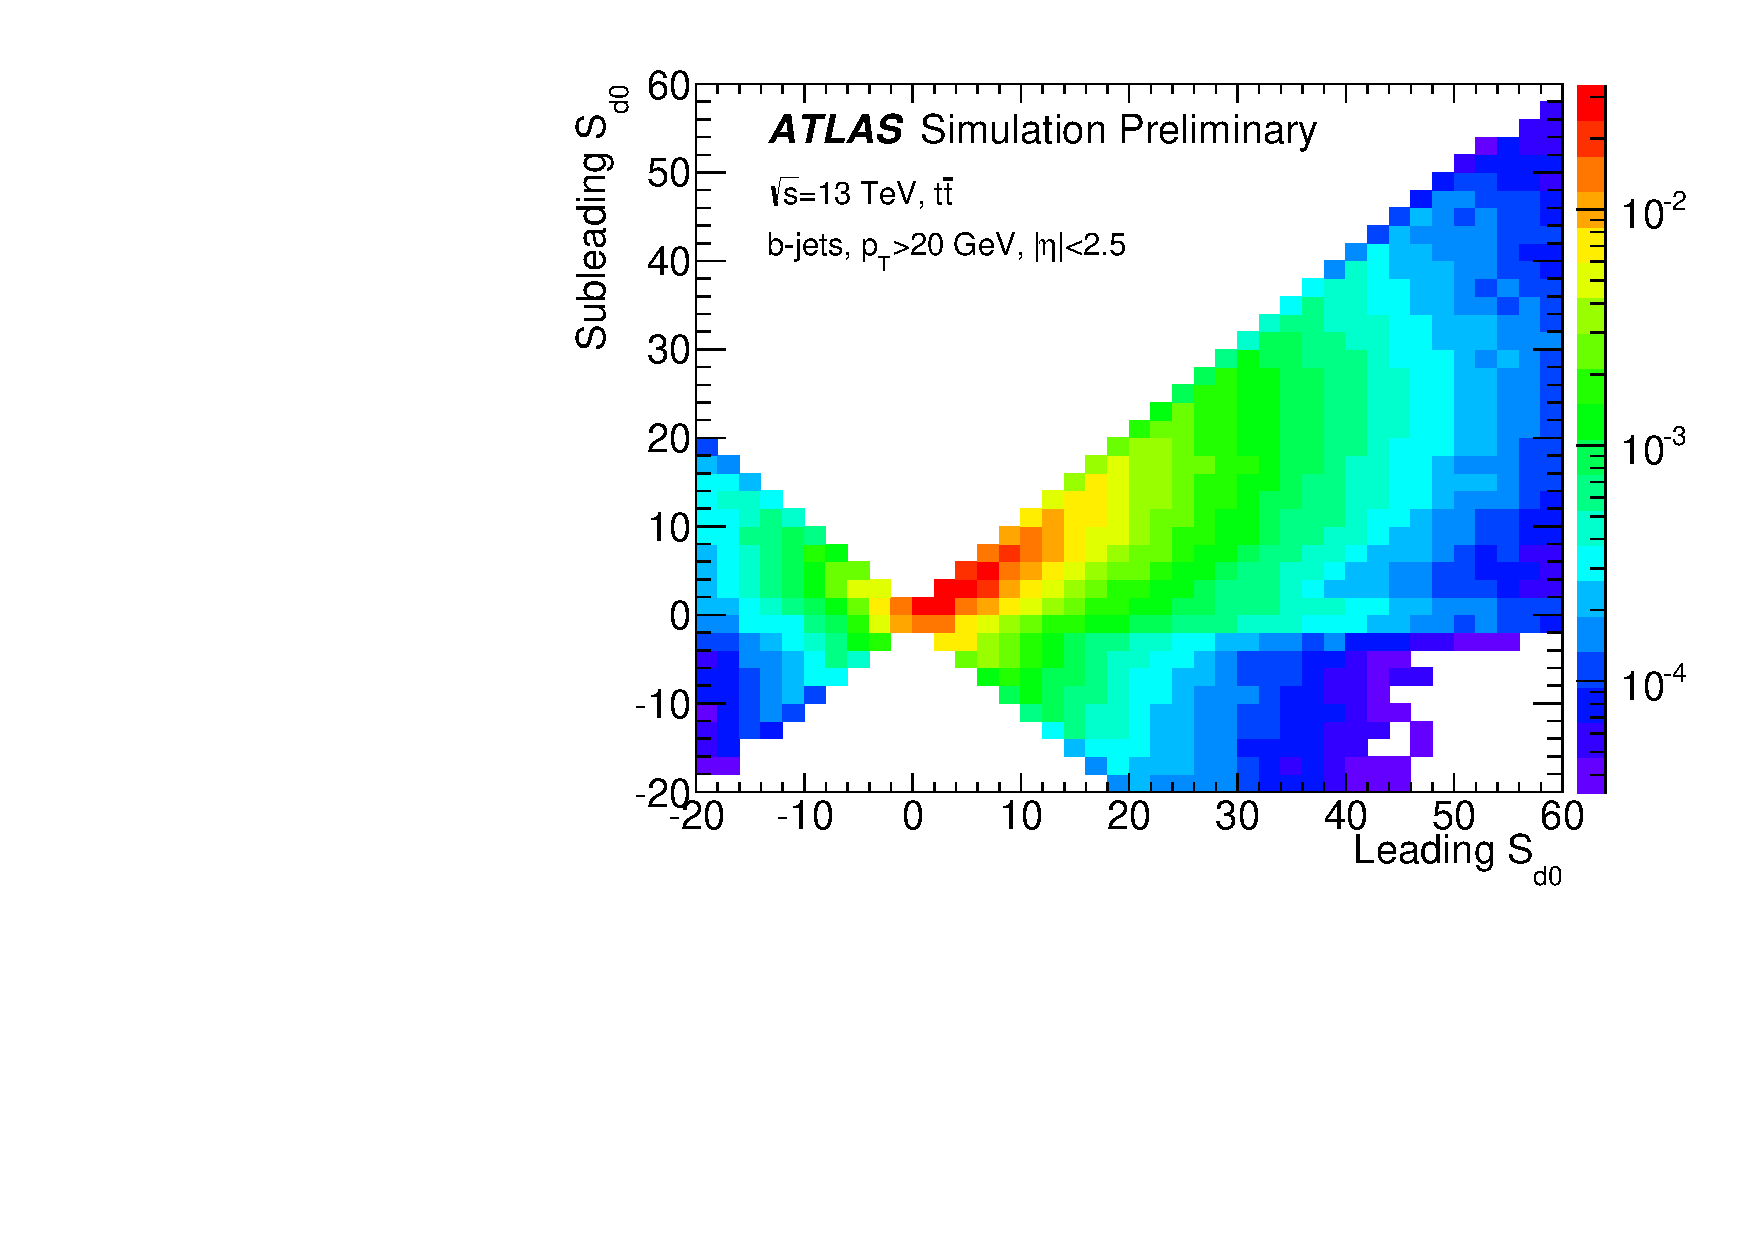
\includegraphics[width=0.48\linewidth]{\figpath/fig_01a}
    } 
     \subfloat[]{ 
            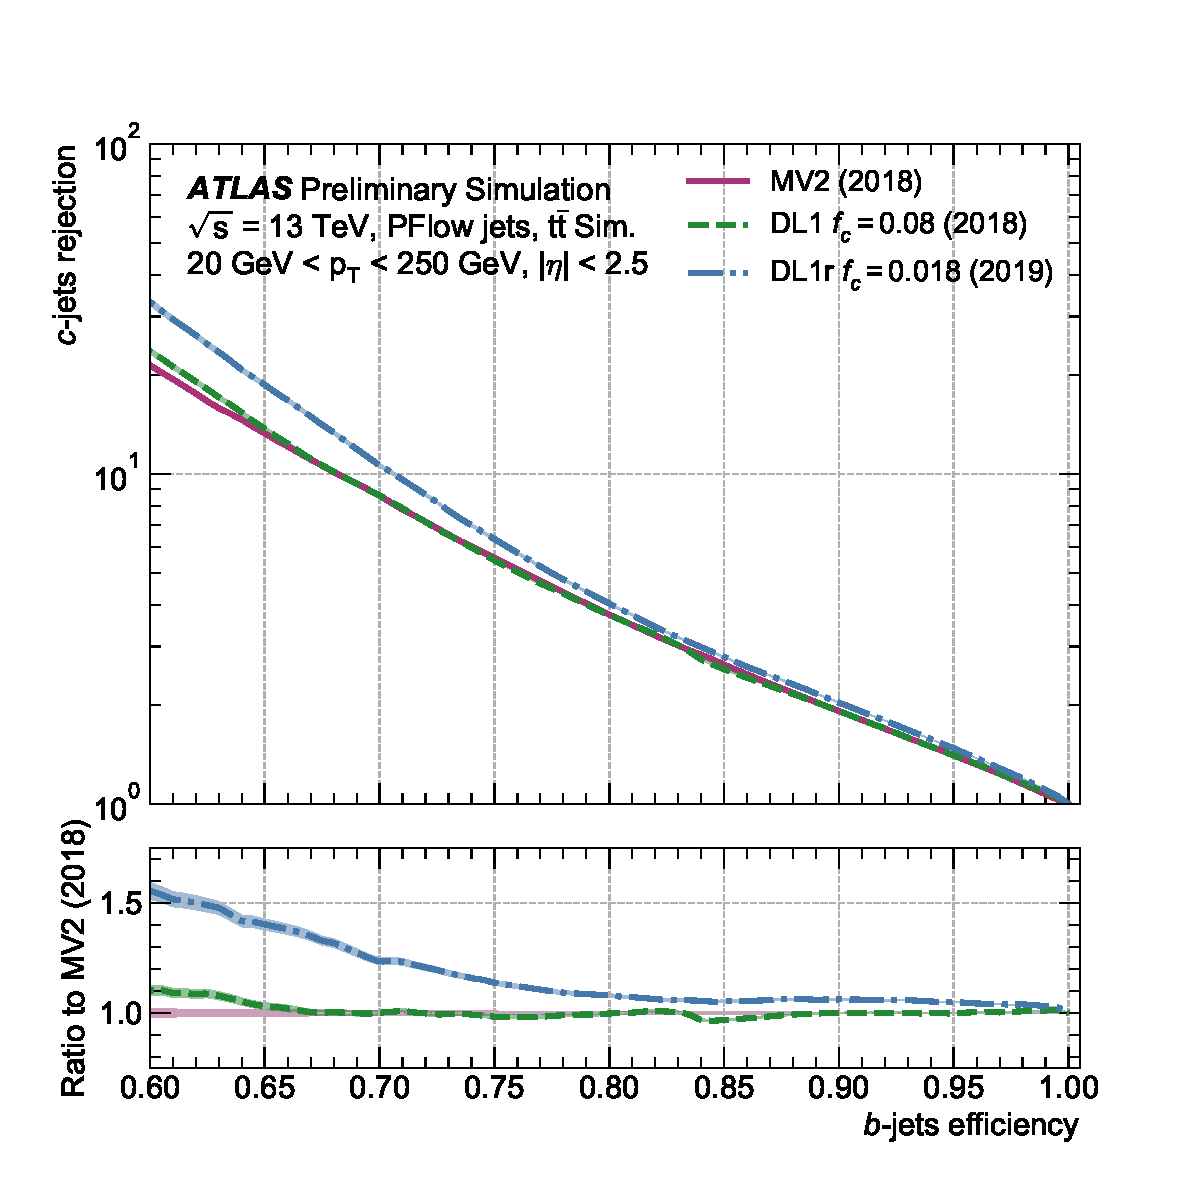
\includegraphics[width=0.48\linewidth]{\figpath/fig_01b}
    } 
    \caption{}
    \label{fig:\jetdef-fig1}
\end{figure}

\begin{figure}[htbp]
    \centering
    % light
    \subfloat[]{ 
            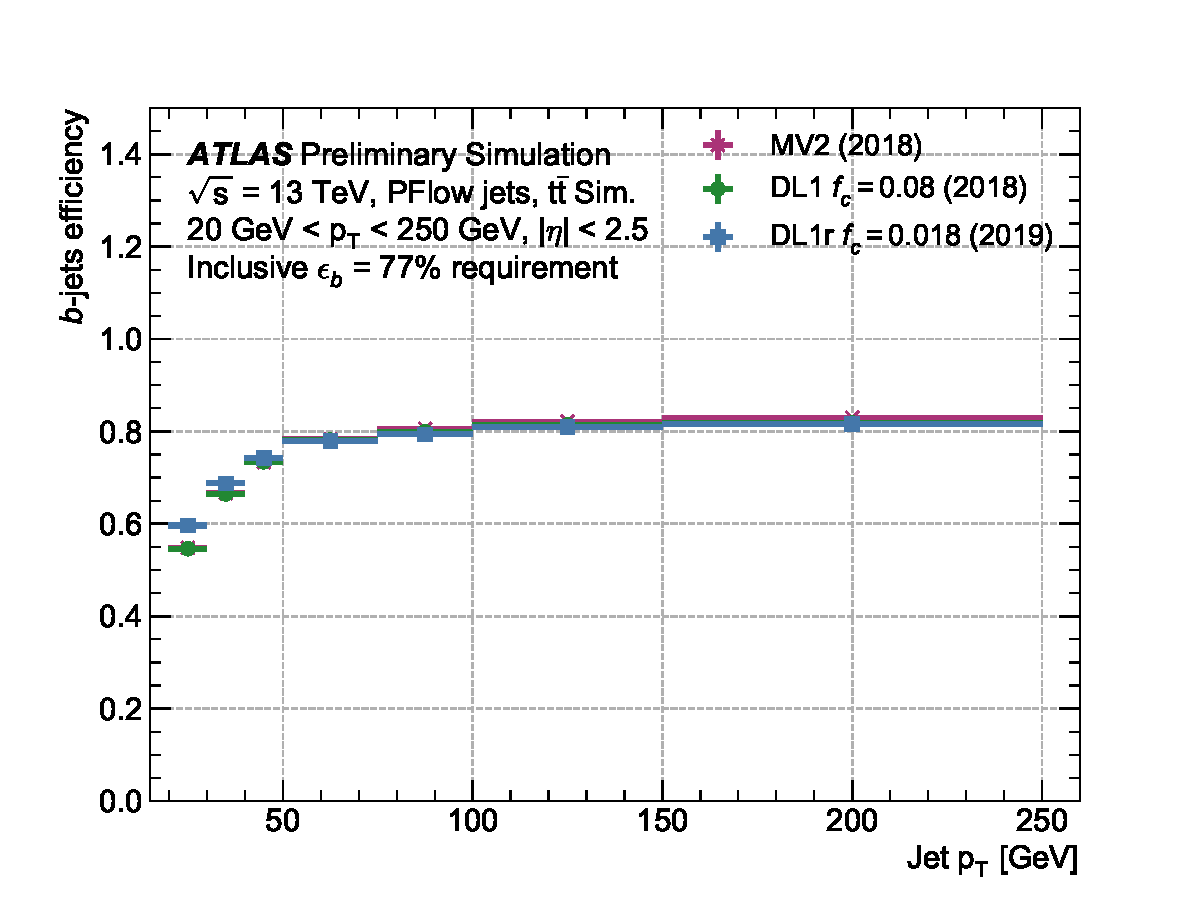
\includegraphics[width=0.33\linewidth]{\figpath/fig_02a}
    } 
     \subfloat[]{ 
            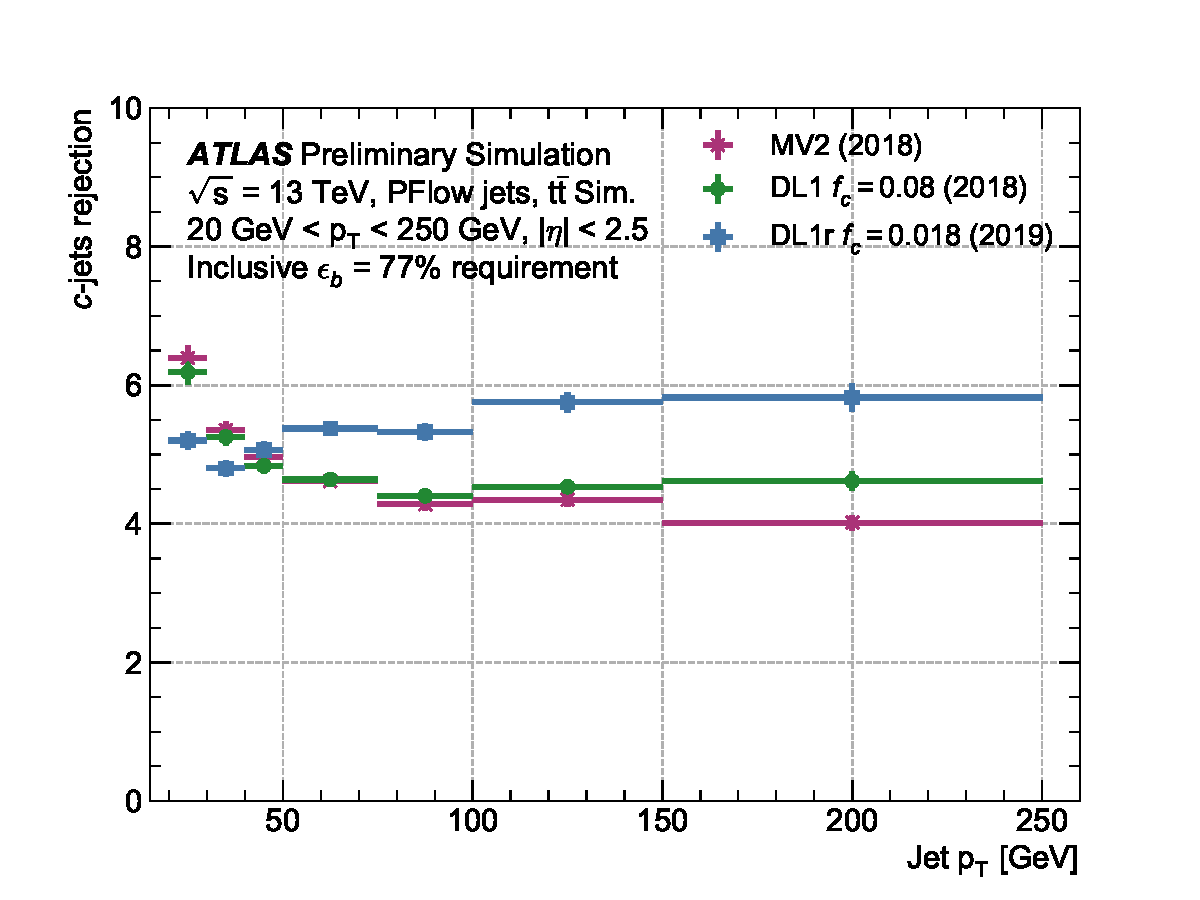
\includegraphics[width=0.33\linewidth]{\figpath/fig_02b}
    } 
    \subfloat[]{ 
            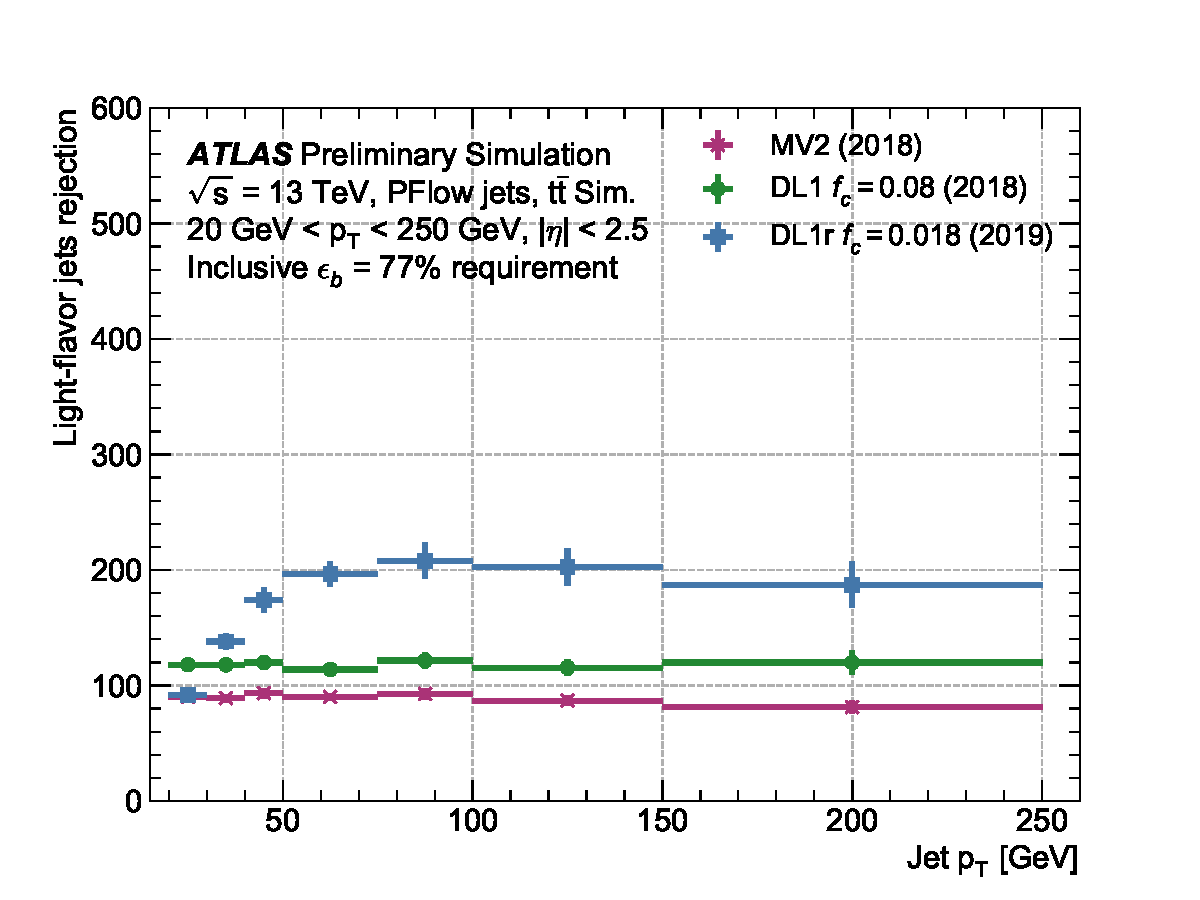
\includegraphics[width=0.33\linewidth]{\figpath/fig_02c}
    } 
    \caption{}
    \label{fig:\jetdef-fig2}
\end{figure}

\begin{figure}[htbp]
    \centering
    % light
    \subfloat[]{ 
            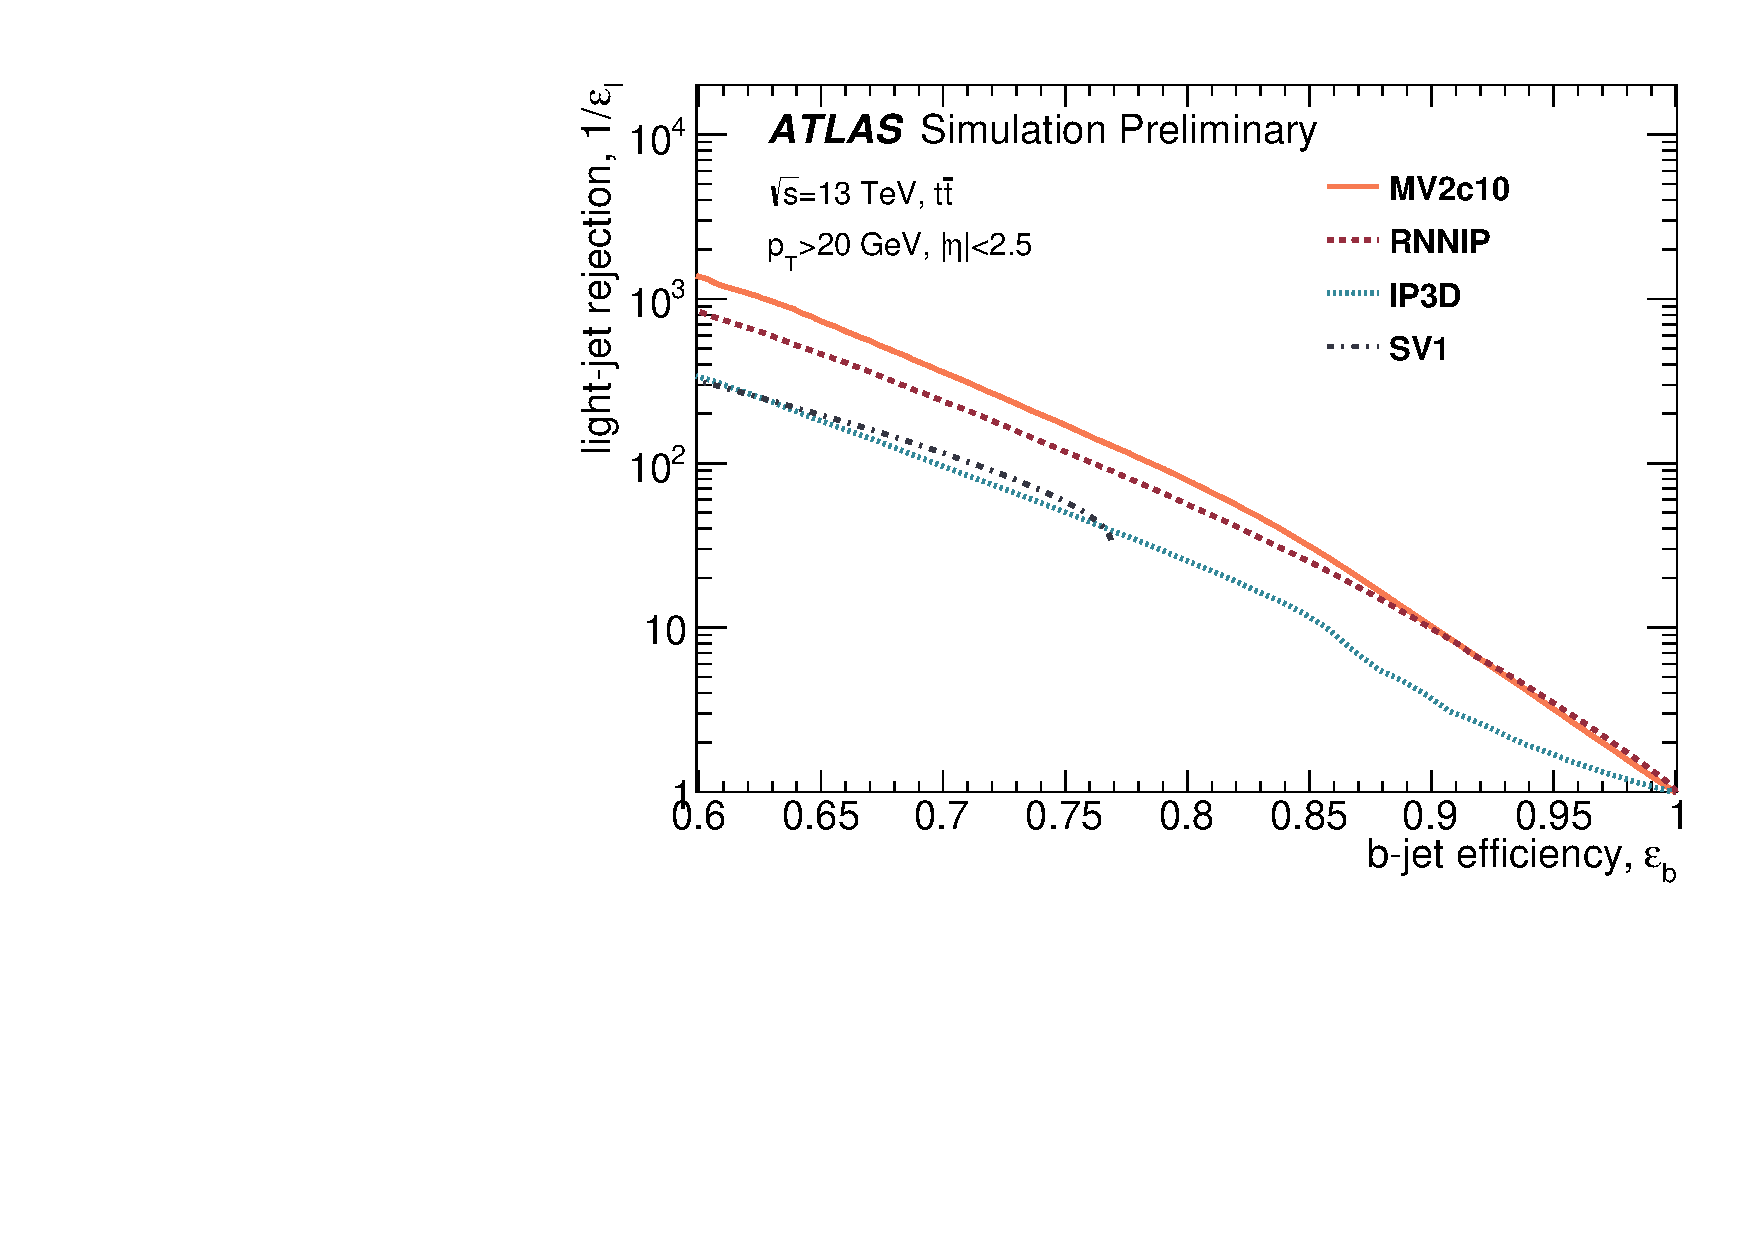
\includegraphics[width=0.48\linewidth]{\figpath/fig_03a}
    } 
     \subfloat[]{ 
            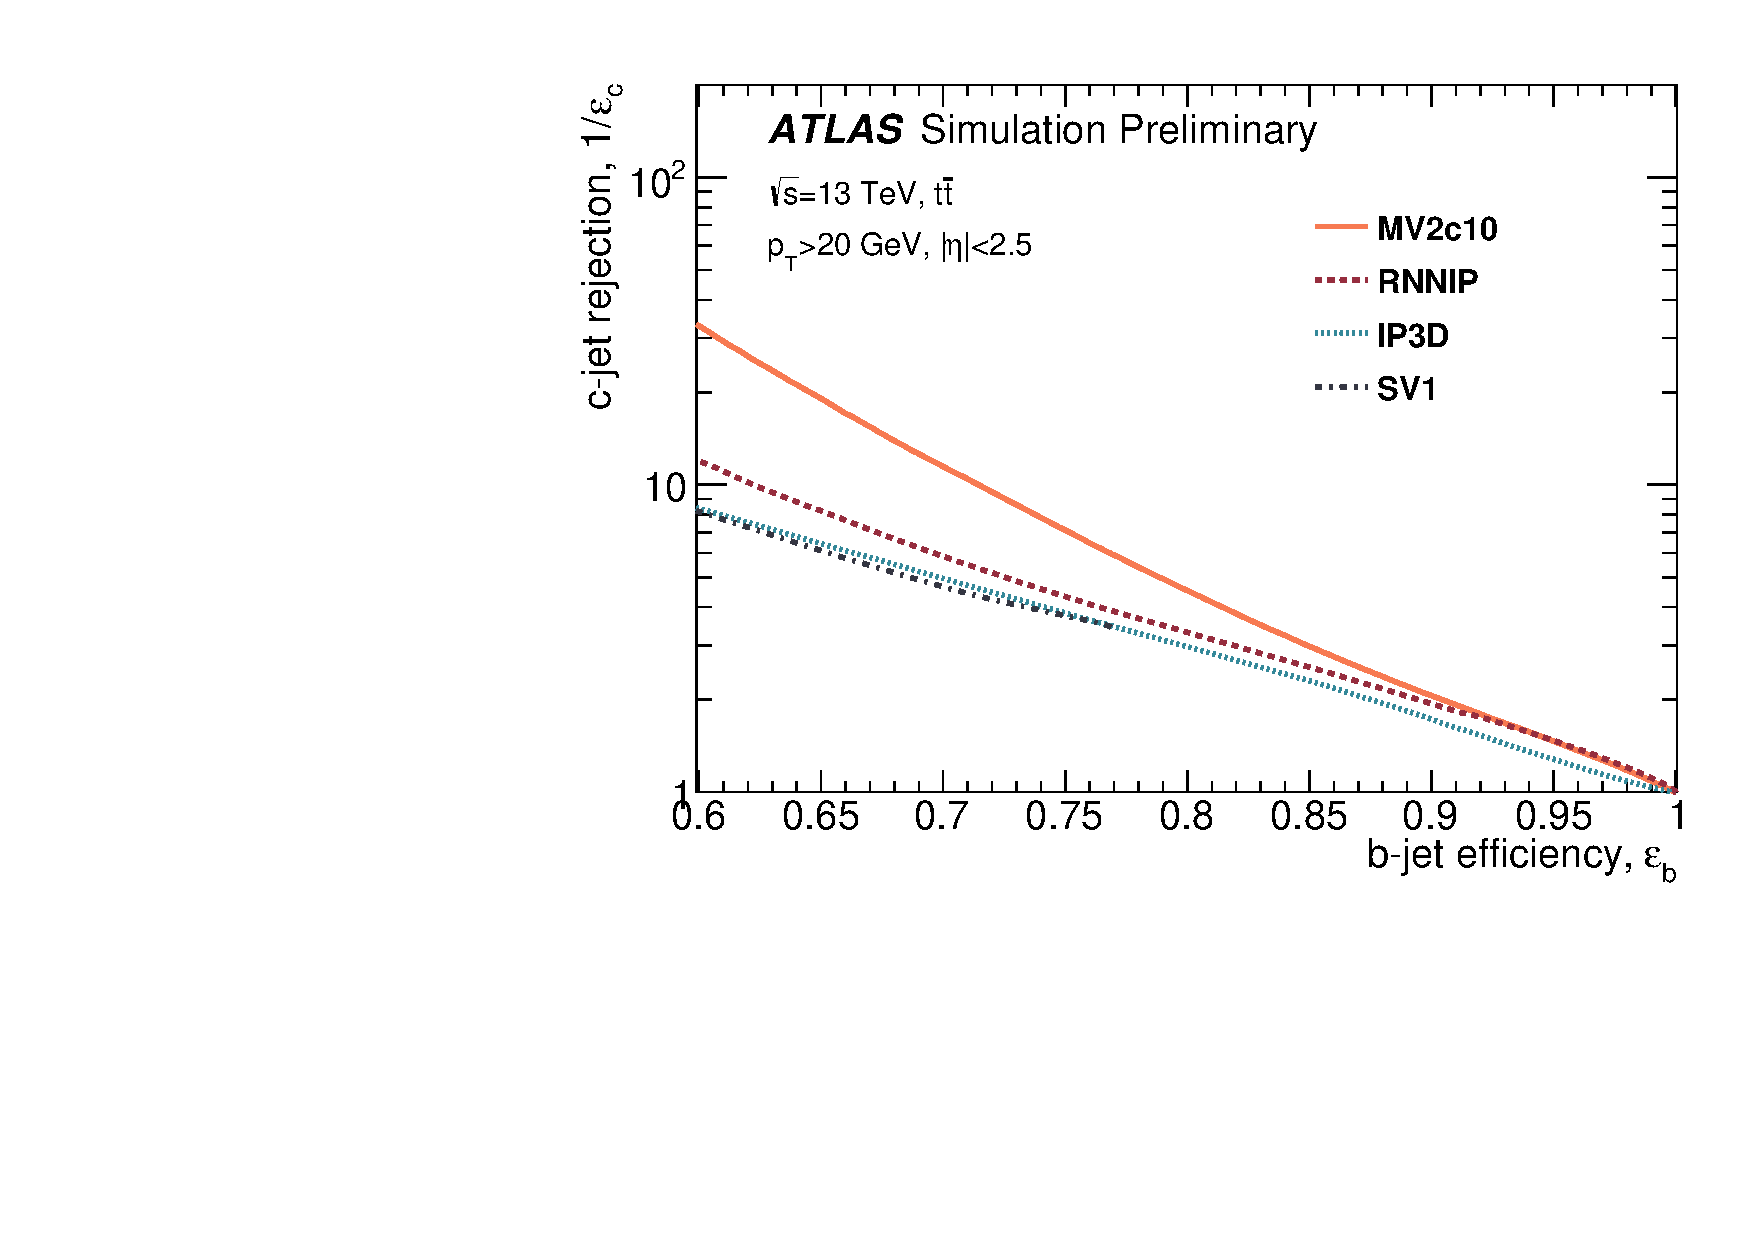
\includegraphics[width=0.48\linewidth]{\figpath/fig_03b}
    } 
    \caption{}
    \label{fig:\jetdef-fig3}
\end{figure}

\subsection{Impact of FTAG improvements on analyses}

\begin{figure}
\centering
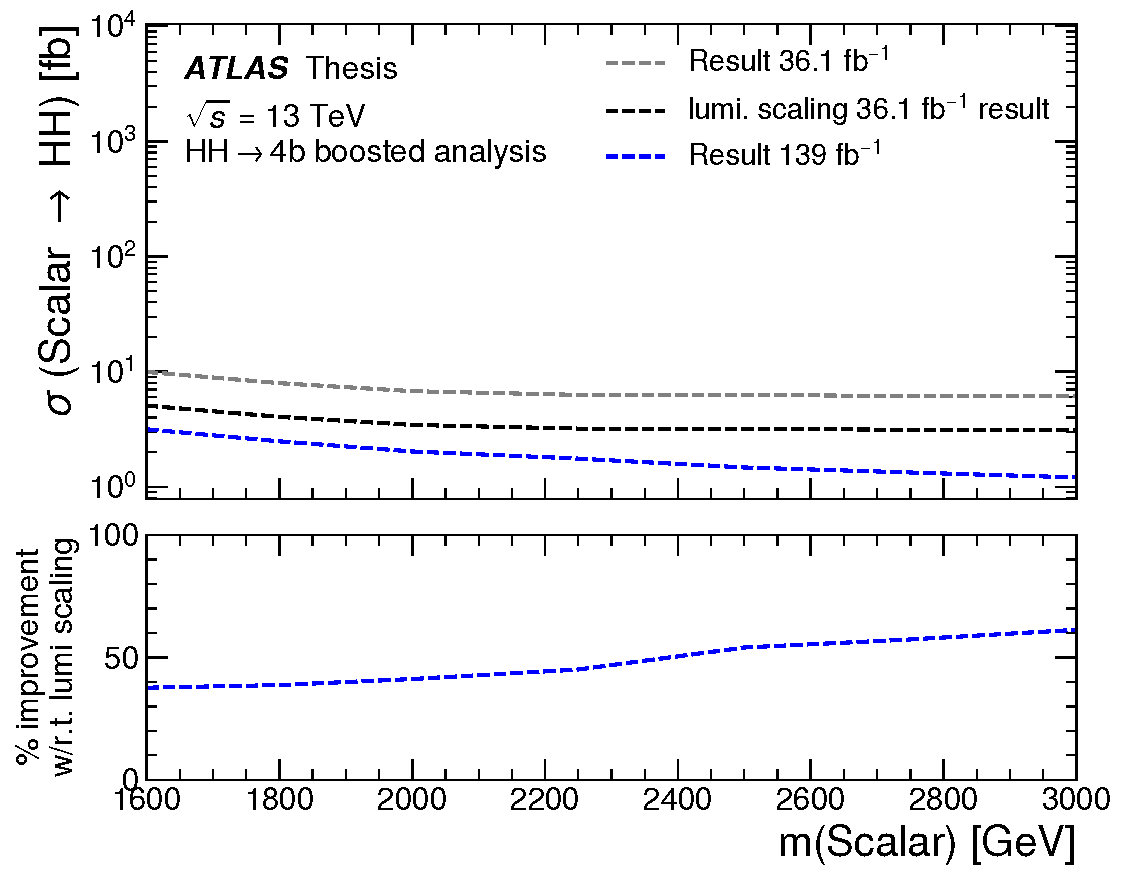
\includegraphics[width=\textwidth]{figures/my_dihiggs/HH4b-boosted-vr-trk-jet-improvements.pdf}
\caption{Need to cite the 36 ifb and 139 ifb.}
\label{fig:boosted-vr-trk-jet-improvements}
\end{figure}


\section{RNNIP calibratability}



\section{Tagger R\&D: DIPS}

% DIPS intro (?) 

This work builds on that of the RNNIP algorithm \cite{ATL-PHYS-PUB-2017-003}, which uses impact parameter information and recurrent neural networks (RNNs) for $b$-tagging, and provides improvements over other IP-based algorithms by accounting for the correlations between the track features, and the inclusion of additional discriminating variables. % impact parameters.
tracks in the jet.
Here a new algorithm is introduced, Deep Impact Parameter Sets (DIPS), based on the Deep Sets architecture \cite{DBLP:journals/corr/ZaheerKRPSS17} and on the application of the Deep Sets formalism within particle physics known as Energy / Particle Flow Networks~\cite{Komiske_2019}.
DIPS solves the same task as RNNIP but treats the tracks in the jet as an unordered, variable-sized set rather than as a sequence, avoiding the need to specify a sequence ordering and the slow processing of RNNs. 
Given that the $b$-hadron decay products do not exhibit any intrinsic sequential ordering, the Deep Sets architecture is also better physically motivated.

DIPS is demonstrated to be as performant as RNNIP but faster to train, decreasing evaluation time and reducing turn-around time for optimization. Therefore, optimization studies of the track selection criteria and new track features are also included.
In addition, a discussion on how to measure the algorithm's efficiency in data, in particular for jets that do not contain a $b$ or a $c$-hadron, is presented. %light flavoured jetsone of the challenges for including machine learning algorithms in our existing workflows is the ability to calibrate them using our existing methods, especially the particularly challenging calibration of the light-quark initiated jet mistag rate, and thus we demonstrate that DIPS is well suited to standard calibration procedures.
Finally, one avenue of research in deep learning models is exploring the interpretability of the models, or trying to dissect what information the network is learning. 
Diagnostic studies from the machine learning literature are presented to demonstrate the well-known characteristics from $b$-quark fragmentation and hadronization process that the network has gleaned.


% --------
% This info can go in the algorithm description part:
% The Deep-Sets implementation, which we denote DIPS (Deep Impact Parameter Sets), exploits a hierarchical organization of the information inside of the jet through separate networks that first operate on the tracks and extract track features and then operate on the jets to take into account correlations with high-level features, but can be trained together end-to-end. 
% --------



\def\figpath{figures/ftag/dips-note/}

\subsection{Algorithm overview}

The Deep Sets architecture~\cite{DBLP:journals/corr/ZaheerKRPSS17}, which treats the elements as a set without any specific order, maintains the benefits of the RNNIP algorithm, while avoiding the required element ordering (which for $b$-tagging is empirically driven rather than strictly dictated by the inputs of the problem).
This architecture was first employed in particle physics in a phenomenological study on the identification of different types of jets~\cite{Komiske_2019}.  
Adopting the formalism of \cite{Komiske_2019}, if $p_i$ is the vector representing the inputs associated with the $i^{th}$ track in the jet, then the Deep Sets architecture applies a neural network (NN) $\Phi$ to each track, sums over the tracks, and then applies additional processing on the summed representation with a feed forward NN $F$, as described in equation~\ref{eq:DeepSets},

\begin{equation}
\mathcal{O}\left(  \{ p_1 , \ldots , p_n \}  \right) = F \left( \sum_{i = 1}^n \Phi \left( p_i \right) \right),
\label{eq:DeepSets}
\end{equation}

where $\mathcal{O} \left(  \{ p_1 , \ldots , p_n \}  \right)$ represents the $b$-, $c$-, and light-flavour class probabilities derived from the inputs for the $n$ tracks in the jet. 
The architecture bifurcates the problem into operations over inputs and operations over sets, where the track-network $\Phi$ extracts the relevant track features, and the jet-network $F$ accounts for the correlations between the tracks. 
The permutation invariance of the set is encoded with the permutation invariant sum operation, although other permutation invariant operations such as the max or average could be used as well. 
The presence of this aggregation layer in the architecture encodes information about track multiplicity inside the jet, which is a useful information for identifying $b$-jets.

This Deep Sets architecture offers the same advantages as RNNIP but encodes permutation invariance between the tracks in the jet, giving a more natural representation of the data and allowing the algorithm to be trained more efficiently with fewer parameters and less data \cite{DBLP:journals/corr/abs-1806-01261}.  
In addition, Deep Sets offers a major additional advantage over RNNs in that the operation of processing the tracks in the jet with the $\Phi$ network can be easily parallelised. 
This allows training and evaluation to make significantly more efficient use of GPUs over the non-parallelisable iterative processing of the RNN. 
The timing performance comparison between DIPS and RNNIP is further discussed in Section \ref{subsec:timing}.
 
\subsection{Implementation details} 
\label{subsec:algdetails}


In this section, algorithms are just trained on $t\bar{t}$ simulated events (described in Section~\ref{sec:datasets}) for multi-class classification between $b$-jets, $c$-jets and light-flavour jets, with the \Pqb and \Pqc-jet distributions reweighted into the light jet distribution. 

For the timing comparisons in Section~\ref{subsec:timing}, the same input features are used for both RNNIP and the DIPS. 
% Additional input features are included for the Optimised DIPS algorithm, described in Section~\ref{subsec:optimisation}. 
The features used in each algorithm are described in Table~\ref{table:inputs}.
The track variables related to the track reconstruction quality focus on the IBL and the next-to-innermost pixel layer (PIX1) due to their strong impact on the IP significance distributions. 
In particular, the number of split hits, which are hits being created by multiple charged particles \cite{PERF-2012-05}, is used to help identify dense tracking environments, in which distinguishing tracks from  heavy flavour decays is generally  more difficult. 
% because these are most crucial for the $b$-tagging performance. 
% The track IP error is highly dependent on whether the track has hits in these first layers and thus impacts the IP significance distributions.

%using the track significances with respect to the PV, some variables characterizing the track kinematics $\pT^{frac} = $ and $\Delta R$ between the track and the (uncalibrated) jet axis, and 9 variables characterizing the hit quality of the track \textbf{list variables}.
%The direct use of the hit information instead of the category from IPXD is a new from \cite{ATL-PHYS-PUB-2017-003} but was what was done for \cite{PFlowPublicPlots2019} which is why this is the RNNIP implementation that we are comparing to. This switch to the hit level information gave a $\mathcal{O}(10\%)$ improvement (keeping everything else in the training setup constant).

After applying the track selections described in Section~\ref{sec:datasets}, the tracks are ordered by decreasing $s_{d0}$, and the first 15 tracks are kept for processing. 
The ordering plays a limited role in the algorithm, since typical jets in the topology investigated should have an average number of tracks that is smaller than the maximum allowed number of tracks (see Table~\ref{table:trkComposition}).
% The number of tracks considered is a trade-off between model complexity, with training and evaluation time growing with this requirement, and algorithm performance.
% for the nominal track selection, while 25 tracks are kept with the looser track selection. 
Since the $\pT^{frac}$ and $\Delta R$ variables have a tail at larger values, the natural log of the value for these variables is used as the feature in order to improve the convergence time of the training.  
Variable normalisation to zero mean and unit variance is frequently used for preprocessing of features in ML algorithms. 
As many of our input variables already have near zero mean, only a subset of the track features are normalised: $\log \pT^{frac}$, $\log \Delta R$, nPixHits, nSCTHits, as well as $d_0$ and $z_0 \sin \theta$ for the optimised DIPS training.

A simplified scheme of the DIPS architecture is shown in Figure~\ref{fig:architecture}, which is based on the architecture in reference~\cite{Komiske_2019}.  
A grid search over the hyperparameters including the number of layers in the $\Phi$ and $F$ networks, the number of nodes in the $\Phi$ and $F$ networks and the dimension of the track latent space revealed similar performance for many different choices of these hyperparameters. 
Both batch normalisation \cite{DBLP:journals/corr/IoffeS15} and dropout \cite{DBLP:journals/corr/abs-1207-0580} were tested, and it was found that batch normalisation was helpful for the DIPS $b$-tagging performance while dropout was not.

\begin{figure}
  \centering
  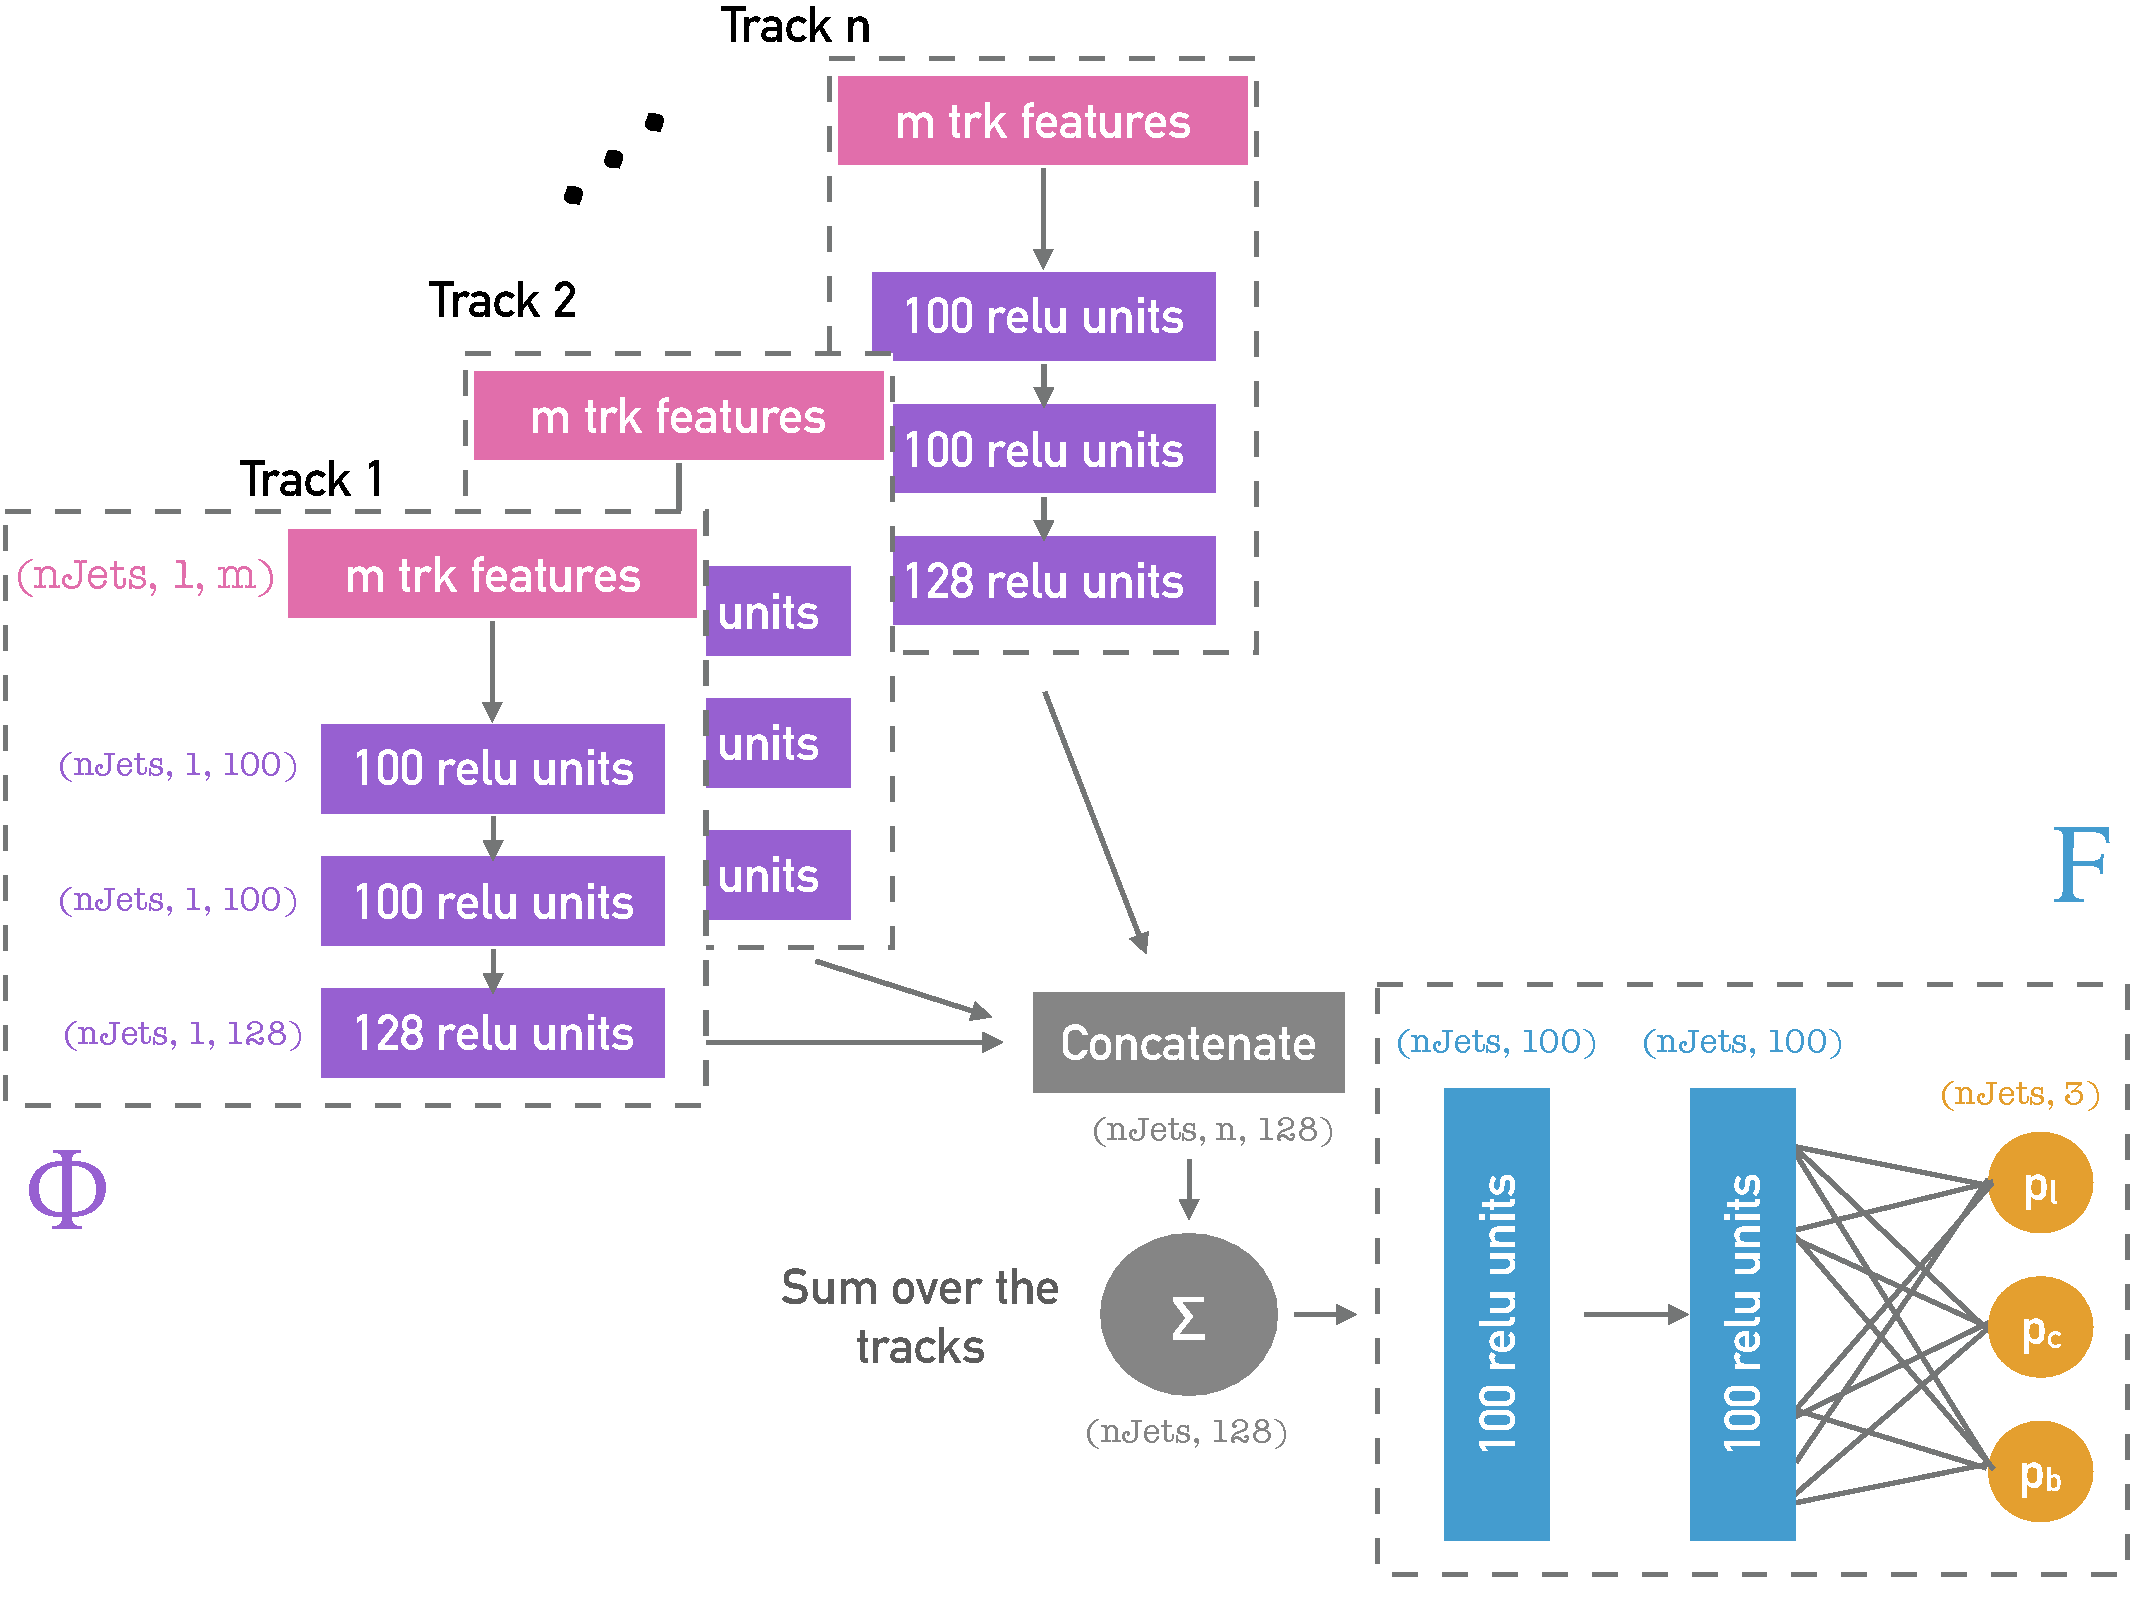
\includegraphics[width=0.8\linewidth]{\figpath/DIPS_architecture}
  \caption{Architecture for the DIPS algorithm. The number of hidden units in the different neural network layers correspond to the final optimized architecture.}
  \label{fig:architecture}
\end{figure}

We present a different training for RNNIP than \cite{ATL-PHYS-PUB-2017-003} and \cite{PFlowPublicPlots2019}, here training on only $t\bar{t}$ for the timing comparisons. RNNIP processes the inputs using an LSTM cell with 100 hidden units, and after processing the sequence, feeds the vector into a feedforward network with 20 units and a dropout fraction of 0.2 before a softmax layer for classification. 

The RNNIP and DIPS trainings were performed with 3 million jets, with 20\% of these jets held out as a validation set to determine when to stop the training. 
After 10 consecutive training epochs (or iterations through the training dataset) without finding a new validation loss minimum, the training is terminated and the model with the best validation loss was selected.  Both the RNNIP and DIPS architectures were implemented in Keras \cite{chollet2015keras} and trained with the TensorFlow backend \cite{tensorflow2015-whitepaper}. 
Algorithms were trained with the Adam optimizer \cite{kingma2014adam} with a learning rate of $10^{-3}$ and a batch size of 256. 
The performance metrics shown in the following sections are obtained with a statistically independent dataset of 3 million jets.

\subsection{Performance}

\subsection{Baseline Performance}
\label{subsec:baseline}

The distribution of the DIPS discriminant $D_b$ (defined in Equation~\ref{eq:dipsdiscriminant}) for each of the jet flavours is shown in Figure~\ref{fig:Db}. 
The peak at $D_b = -1.3$ is due to jets without any selected tracks. 
Clear separation between the distribution of $b$-jets and light-flavour jets can be seen, as well as a strong but smaller separation between $b$-jet and $c$-jets as expected due the similarities between $b$-hadron and $c$-hadron decays.

\begin{figure}[h!]
  \centering
  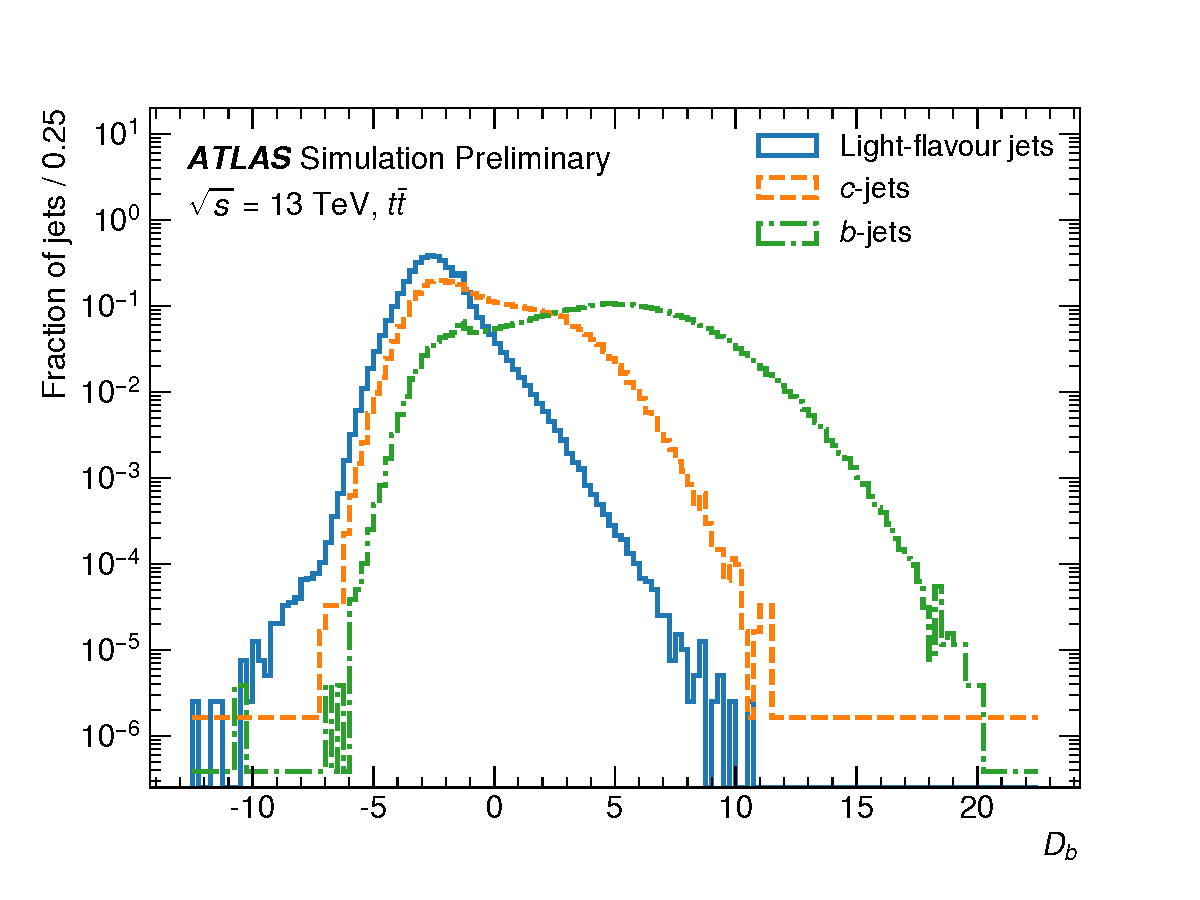
\includegraphics[width=0.5\linewidth]{\figpath/disc_DIPS_phi_100_100_128_F_100_100_3out_bn_3mtrain_15trks_sd0_sz0_nNextToInnHits_nInnHits_nsharedBLHits_nsplitBLHits_nsharedPixHits_nsplitPixHits_nsharedSCTHits_logNorm_ptfrac_dr_norm_nPixHits_nSCTHits_iter1}
  \caption{Distributions of DIPS $b$-tagging discriminant, as defined in Equation \ref{eq:dipsdiscriminant}, for $b$-jets, $c$-jets and light-flavour jets.}
  \label{fig:Db}
\end{figure}

The performance of taggers can be examined and compared through a Receiver Operator Characteristic (ROC) curve: a scan is performed for a threshold $\tau$ on $D_b$, and the efficiency for $b$-jets at each threshold is computed as the fraction of $b$-jets with $D_b > \tau$, while the rejection of $c$-jets or light-flavour jets is computed as one over the fraction of $c$-jets or light-flavour jets (inverse mistag efficiency), respectively, with $D_b > \tau$. 
The $b$-jet efficiency and light-flavour (or $c$) jet rejection for the same $\tau$ are then plotted.  Each model is trained five times and for a given $b$-jet efficiency, the mean of the rejections is used as the nominal value and the standard deviation of the rejections is used for the width of the curve. 
This ensemble of trainings is known to assess the predictive uncertainty of machine learning-based algorithms~\cite{deepensembles}.

The ROC curves for $b$-jet efficiency versus light-flavour jet rejection and for $b$-jet efficiency versus $c$-jet rejection of the DIPS and RNNIP algorithms are shown in Figure~\ref{fig:roc_rnnip_dips}. 
% The width of the curves is calculated by repeating the algorithm training five times with different random weights
The lowest $b$-jet efficiency displayed corresponds to the lowest efficiency benchmark used in physics analyses within the ATLAS experiment. 
%, and Figure~\ref{fig:roc_rnnip_dips} also includes the Optimised DIPS discussed in Section~\ref{subsec:optimisation}. 
The DIPS algorithm provides up to a 15\% additional light-flavour jet rejection and a 5\% additional $c$-jet rejection at a given $b$-jet efficiency over the RNNIP algorithm. 
Notably, as will be discussed in Section~\ref{subsec:timing}, this similar performance comes with a significant decrease in training and evaluation time.

\begin{figure}[ht]
    \centering
    \subfloat[]{ 
            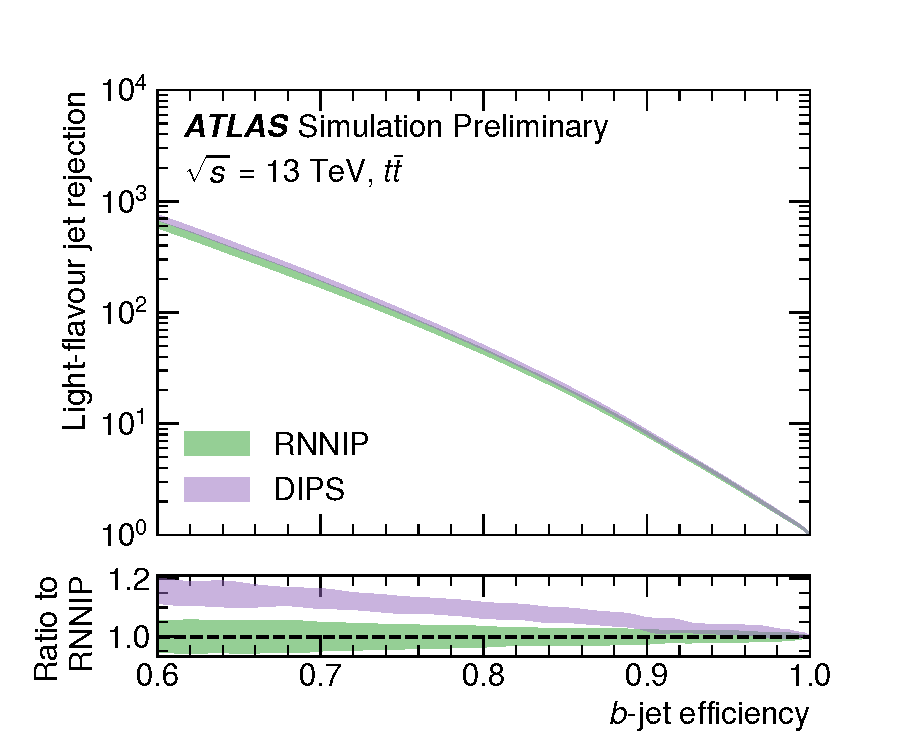
\includegraphics[width=0.48\textwidth]{\figpath/rocAvgIter_l_rnnip_dips}
    }   
    \subfloat[]{ 
            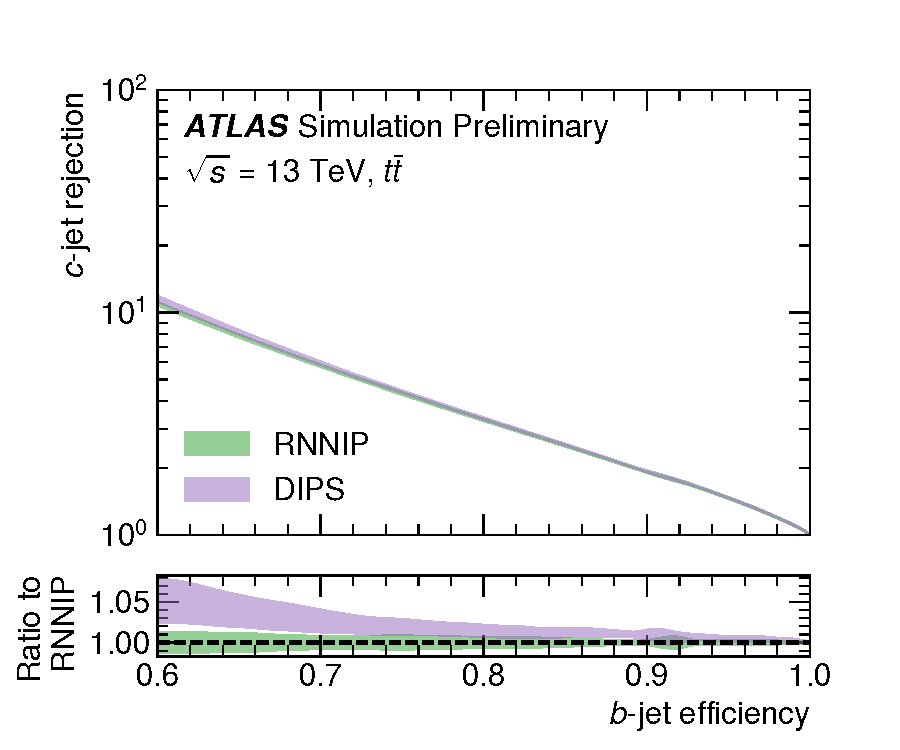
\includegraphics[width=0.48\textwidth]{\figpath/rocAvgIter_c_rnnip_dips}
    }   
    \caption{Light-flavour jet rejection as a function of $b$-jet efficiency (a) and $c$-jet rejection as a function $b$-jet efficiency (b) of the RNNIP (green) and DIPS (purple) algorithms. The central curves and error bands show the mean and standard deviation, respectively, of the rejection at each $b$-jet efficiency for 5 trainings. The ratios are computed with respect to the RNNIP ROC curve.}
    \label{fig:roc_rnnip_dips}
\end{figure}

In order to explore what DIPS is learning in the correlations between features that aids the classification performance, the average saliency map for $b$-jets with 8 associated tracks and failing a threshold corresponding to 77\% $b$-tagging efficiency is shown in Figure~\ref{fig:saliency}. 
The saliency map is computed as 
\begin{equation}
\frac{\partial D_b}{\partial x_{ik}} = \frac{1}{N} \sum_{j=1}^N \frac{\partial D_b^{(j)}}{\partial x_{ik}^{(j)}}, 
\label{eq:salmap}
\end{equation}
and is the gradient of the discriminant value $D_b^{(j)}$ with respect to each track feature input $x_{ik}^{(j)}$, averaged over jets ($j$) in a sample of N jets~\cite{simonyan2013deep}.  
In this case, the feature inputs are normalized to zero mean and unit variance, in a similar way to the training procedure. 
The saliency map gives a linearised view of how the discriminant value is sensitive to changes in the inputs. Figure~\ref{fig:saliency} thus shows how  this sample of $b$-jets which failed tagging could be modified to make them more $b$-jet like.
One can see there is a reasonably strong positive gradients for the significances ($s_{d0}$ and $s_{z0}$) extending up to 5 tracks, which is the average number of charged particle tracks in a $b$-hadron decay. 
Beyond 5 tracks, the gradients for all features are either nearly zero or negative, indicating that either these tracks provide no further information or that tracks with large feature values are more indicative of background. 
In addition, DIPS is highly sensitive to the $\log \pT^{frac}$ and $\log \Delta R$ of the leading $s_{d_0}$ track, which is consistent with the harder fragmentation of $b$-quarks with respect to light-flavour and charm jets. Interestingly, this strong correlation with $\log \pT^{frac}$ and $\log \Delta R$ for the highest $s_{d_0}$ track also indicates that simply enlarging the IPs of a track in a jet would not directly lead to a jet passing a tagging threshold, as the track must also be consistent with the kinematic expectations from $b$-jet fragmentation.
The gradients for the shared and split hits of the high $s_{d0}$ tracks are strongly negative since tracks formed from random combinations of hits are more likely in highly dense environments.
It can also be seen that the correlation with the overall number of hits in the inner most pixel layers, IBL and PIX1, is positive but small. Such features are of high importance to the estimate of the IP and IP resolution. However such information is also encapsulated in the IP significance features which are strongly correlated with the discriminant. 
We suspect these correlations are observed to be relatively small due to the discriminator heavily relying on the IP significance for the first order estimate of the quality of the track and the track's utility for classification.
%indicating that we want the high $s_{d0}$ tracks to have good quality so that they are less likely to have been constructed from a random combination of hits in the tracker.
%For the hit variables encoding the quality of the tracks, we want the high $s_{d0}$ tracks to be high quality, i.e, not have hits that are shared or split which is more common for fake tracks c
% However, the gradients of the raw number of hits in the IBL, PIX1, pixel and SCT detector are not as strong, as real $b$-hadrons in $t\bar{t}$ may have sufficient momentum to decay after the IBL (or PIX1).

\begin{figure}[htbp!]
    \centering
    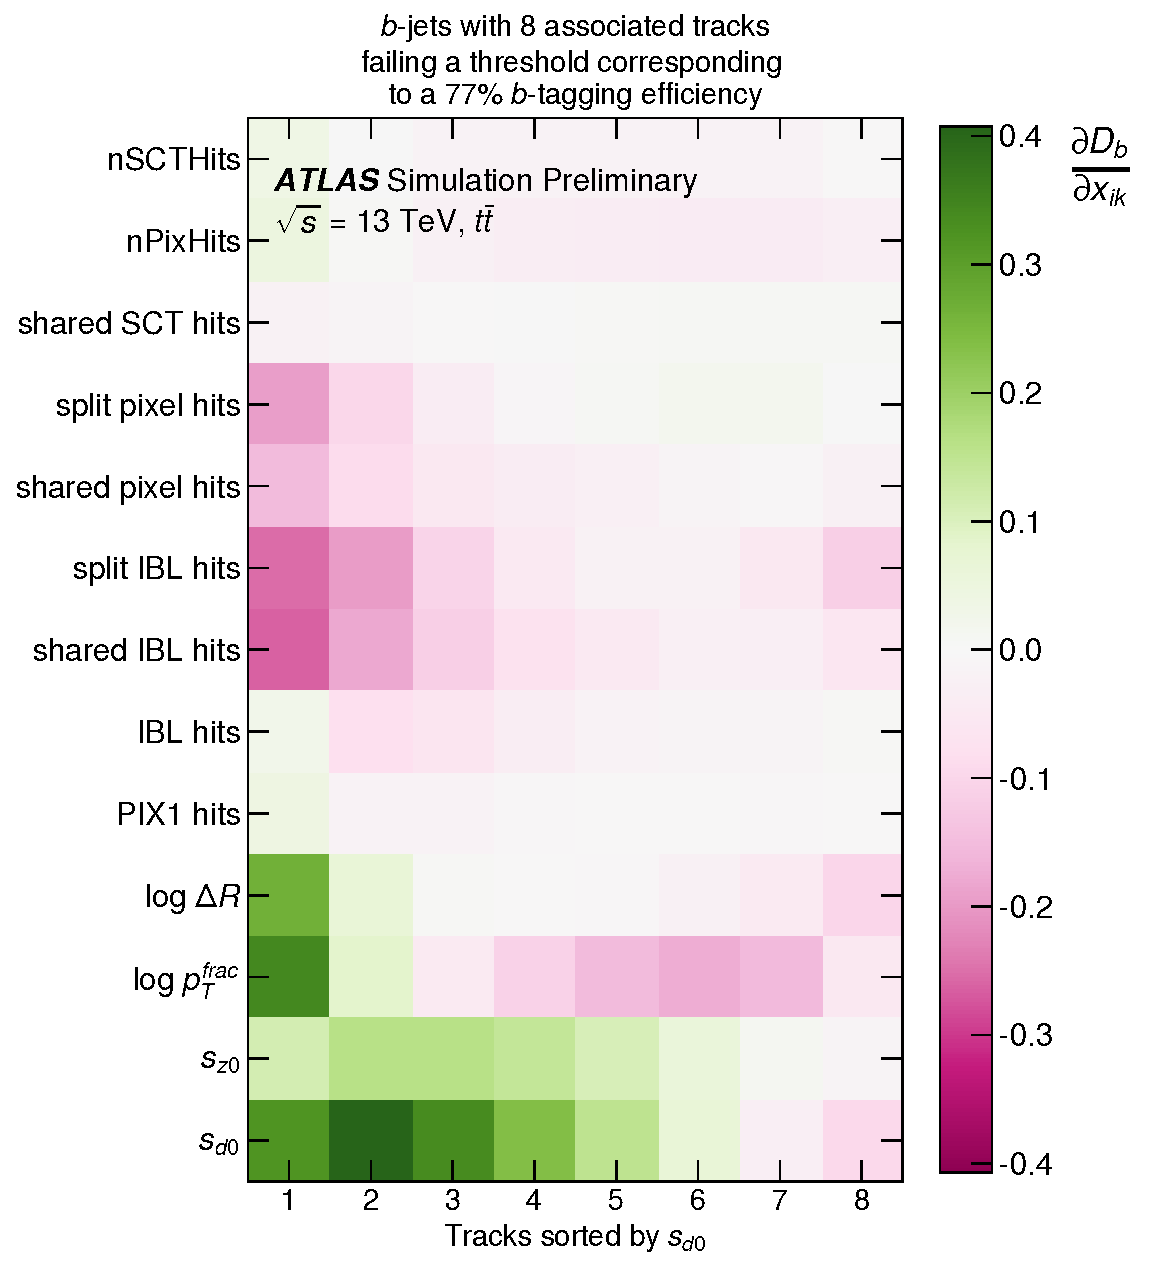
\includegraphics[width=0.8\linewidth]{\figpath/saliency/mc16d_PFlow_BTagging201903_ttbar_pt_1000_d0_1_z0_1.5/Db/noNorm/img_misID_b_77WP_8trks}
    \caption{Saliency map for $b$-jets with 8 tracks. The track features are shown on the $y$-axis, the tracks (ordered by $s_{d_0}$) are listed on the $x$-axis. The colors in each pixel represent the gradient defined in Equation \ref{eq:salmap}. }
    \label{fig:saliency}
\end{figure}


\subsection{Time comparison}
\label{subsec:timing}

A further key comparison metric between the RNNIP and DIPS algorithms is the time needed for training and evaluation. 
The training time limits the ability to critically perform optimisation tests and compare model variants, while the evaluation time impacts ATLAS reconstruction time when deployed at scale and the ability to use such algorithms in low-latency environments such as the trigger. 
The DIPS and RNNIP models with comparable numbers of parameters are compared in terms of their speed of training and evaluation in Tables~\ref{tab:timingGPUs} and~\ref{tab:timingGPUs_eval}, respectively. 
Training comparisons are done on an NVIDIA 2080 Ti GPU, while evaluation comparisons are performed on an NVIDIA Titan X GPU. 
Five versions of each model are trained and evaluated, and the mean and standard deviation of the training and evaluation time is reported. 
A significant speed up of more than a factor of 2 for the DIPS algorithm over RNNIP is observed. 
As training also involves the early stopping procedure, and thus each algorithm may train for a different number of epochs, the training time per epoch is also reported and shows more than a factor of 3 faster speed for DIPS over RNNIP. 
This is similar to evaluation time, where DIPS is seen to be nearly a factor of 4 faster than RNNIP.

\begin{table}[htbp!]
  \begin{center}

    \begin{tabular}{l | c | c | c } % <-- Alignments: 1st column left, 2nd middle and 3rd right, with vertical lines in between
      \textbf{Model} & \textbf{Parameters} & \textbf{Training time [min]} & \textbf{Time / epoch [s]}  \\
      \hline
      RNNIP & 47k & $86 \pm 13$ & $241 \pm 14$  \\
      DIPS    & 49k & $44 \pm 4$ & $78 \pm 4$  \\
    \end{tabular}
    \caption{Timing metrics for trainings performed on Nvidia 2080 Ti GPUs. The nominal value denotes the mean of five independent trainings, while the error bar is the standard deviation.}\label{tab:timingGPUs}
  \end{center}
\end{table}

\begin{table}[htbp!]
  \begin{center}
     \begin{tabular}{l | c | c | c } % <-- Alignments: 1st column left, 2nd middle and 3rd right, with vertical lines in between
      \textbf{Model} & \textbf{Parameters} & \textbf{GPU Evaluation time [s]} & \textbf{CPU evaluation time [s]}  \\
      \hline
      RNNIP & 47k   & $170 \pm 2$ & $685\pm84$  \\
      DIPS    & 49k & $46 \pm 2$ & $206\pm98$ \\
    \end{tabular}
    \caption{Timing metrics for the full test dataset (3 million jets) with GPU evaluations on an NVIDIA Titan X GPU. The nominal value denotes the mean of five independent trainings, while the error bar is the standard deviation.}\label{tab:timingGPUs_eval}
  \end{center}
\end{table}

\subsection{Calibratability}
\label{subsec:calibratability}

While performance in simulation gives an important view of an algorithm's performance, ultimately its efficiency must be calibrated to data. 
This is done using control samples built with specific event selections for each flavour of jet and comparing the observed and simulated efficiency. 
This is especially challenging for light-flavour jets, as it is difficult to identify a highly pure sample of such jets after the $b$-tagging requirement. 

A large fraction of light-flavour jets are wrongly classified as $b$-jets due to tracks being on the tail of their IP distribution and are thus mismeasured. 
%This effect has equal probability for mismeasuring a track as having positive or negative lifetime sign, leading to symmetric IP distributions (as seen in Figure~\ref{fig:flippedInputs}). 
This effect is mostly coming from sources, such as detector resolution and pile-up collisions, which have equal probability for mismeasuring a track as having positive or negative lifetime sign, leading to mostly symmetric IP distributions (as seen in Figure~\ref{fig:flippedInputs}).
As such, a data augmentation procedure called \textit{flipping} can be applied whereby the sign of track IPs (and that of secondary vertices) is multiplied by -1, without affecting the overall light-flavour jets IP distributions~\cite{ATLAS-CONF-2018-006}.
The tagger evaluated on flipped inputs, the \textit{flipped} tagger, will then have an approximately equal performance in light-flavour jets as the nominal tagger.
However, for $b$-jets and $c$-jets with real large IP tracks, the flipping will lead to large changes in their asymmetric IP distribution, with significantly fewer large IP tracks, causing the flipped tagger to be inefficient for identifying these jets. 
Therefore, applying a $b$-tagging requirement on the flipped tagger will generate a dataset with a higher fraction of light-flavour jets, when compared to the dataset built with the nominal tagger, such that the light-flavour jet efficiency can be obtained in data. 
In order for this to succeed, the $b$-tagging algorithms must uphold this approximate flipping symmetry of the light-flavour jets in their prediction, while reducing $b$-jets and $c$-jets tagging efficiencies.

The discriminant distributions of $b$-jets, $c$-jets and light-flavour jets with nominal and flipped inputs for the RNNIP and DIPS algorithms are shown in Figure~\ref{fig:flippedDisc}. 
The dashed vertical lines represent the discriminant requirement for 85\%, 77\%, 70\% and 60\% inclusive $b$-jet efficiencies, corresponding to the efficiency benchmarks used at analysis level. 
The desired properties are found for both DIPS and RNNIP, the flipped distribution for light-flavour jets is nearly unchanged, while there is a significant decrease in flipped $b$-jets and $c$-jets at high discriminant values. 
Using these distributions, the efficiencies of the different jet flavours as a function of the RNNIP or DIPS discriminants can be examined, as in Figure~\ref{fig:rocFlippedTaggers}.  
For both DIPS and RNNIP, one can see the large reduction on the efficiency for selecting $b$-jets and $c$-jets for a fixed light-flavour jet rejection as desired.

\begin{figure}[htbp]
    \centering
    % light
    \subfloat[]{ 
            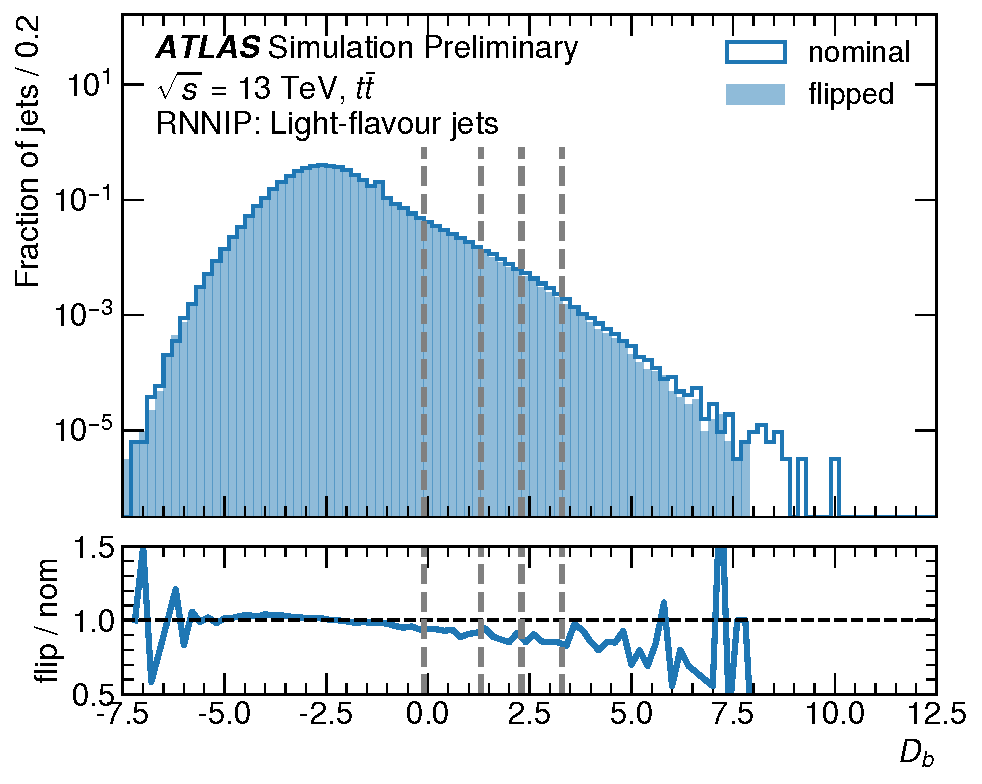
\includegraphics[width=0.41\linewidth]{\figpath/cf_Light-flavour_disc_rnn_flip}
    } 
     \subfloat[]{ 
            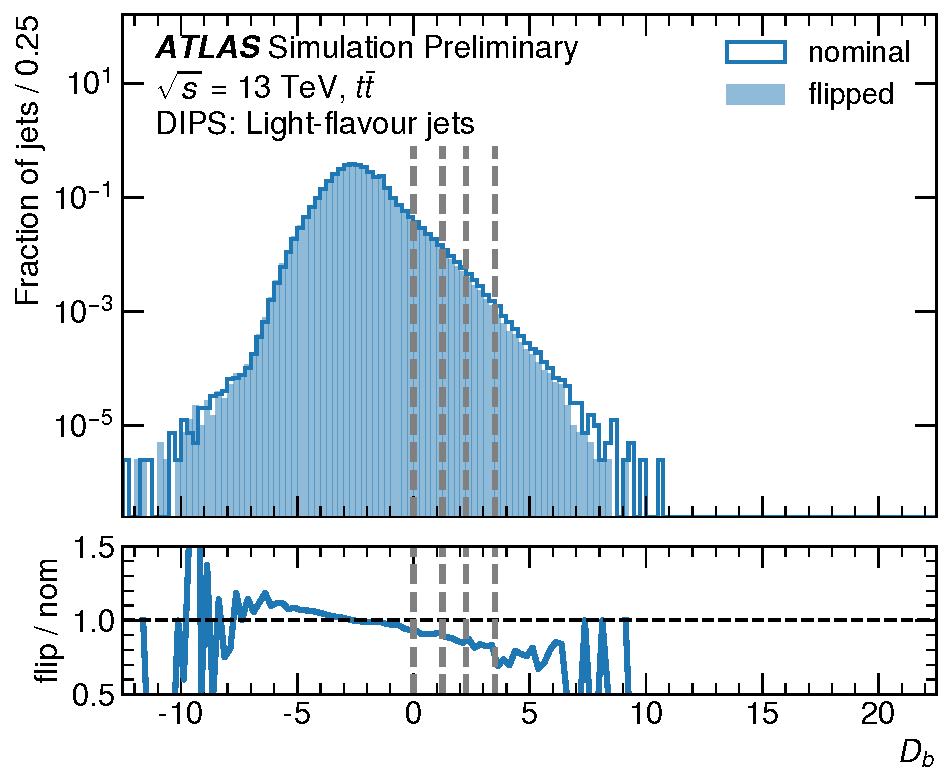
\includegraphics[width=0.4\linewidth]{\figpath/cf_Light-flavour_disc_dips_flip}
    }  \\
    % charm
    \subfloat[]{
            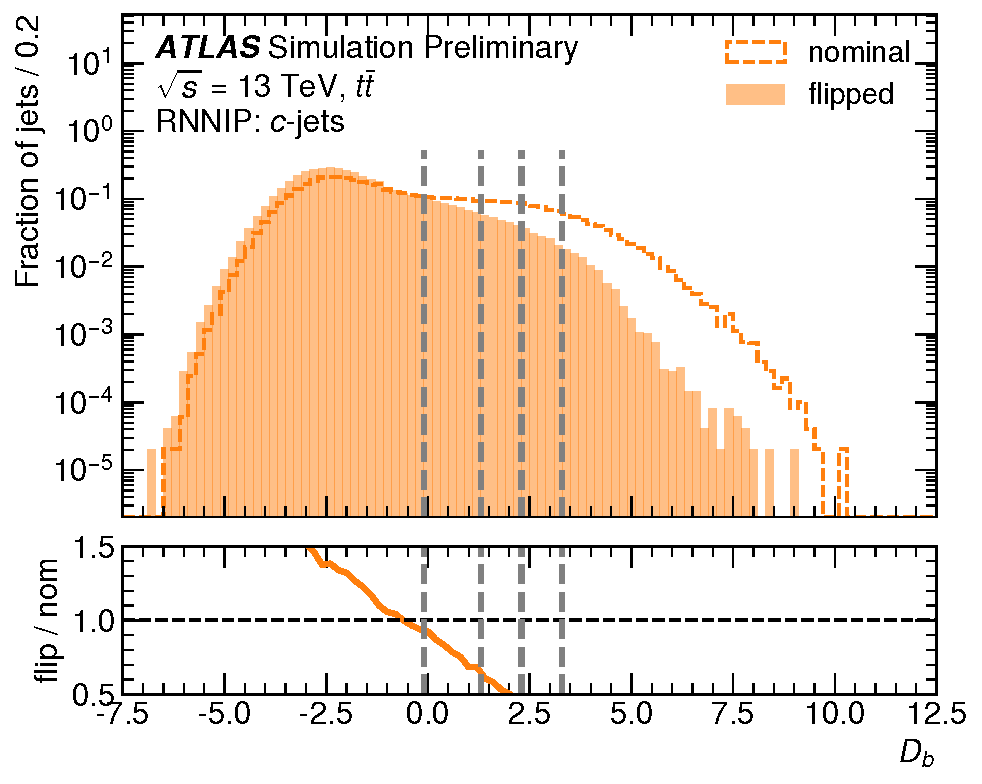
\includegraphics[width=0.41\linewidth]{\figpath/cf_$c$_disc_rnn_flip}
    }   
    \subfloat[]{ 
            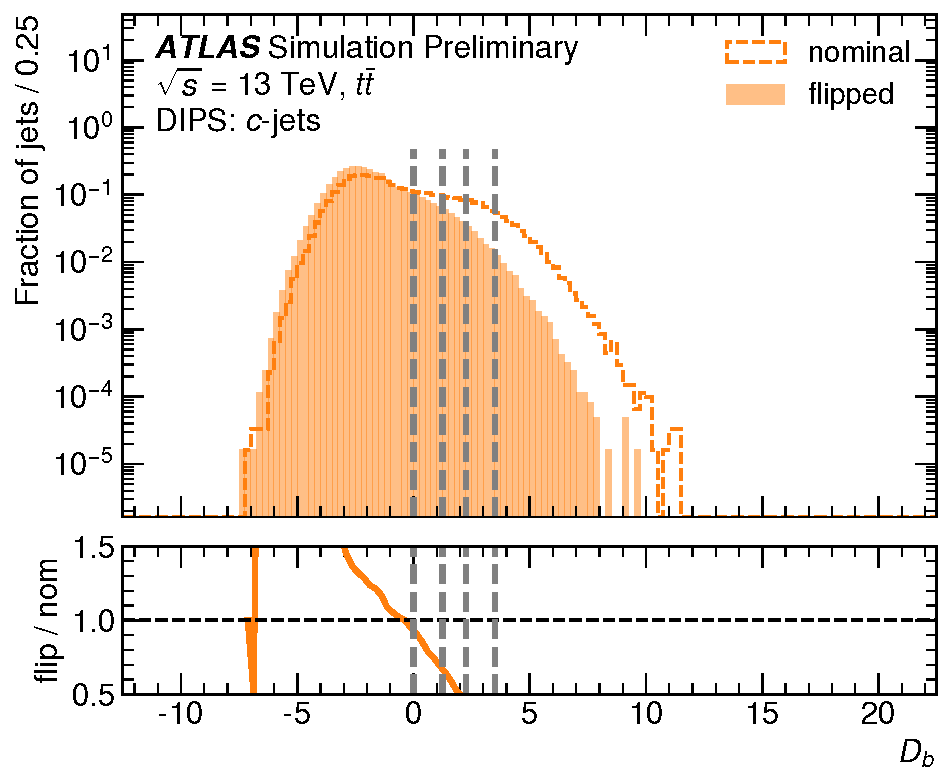
\includegraphics[width=0.4\linewidth]{\figpath/cf_$c$_disc_dips_flip}
    } \\
    % b
    \subfloat[]{
            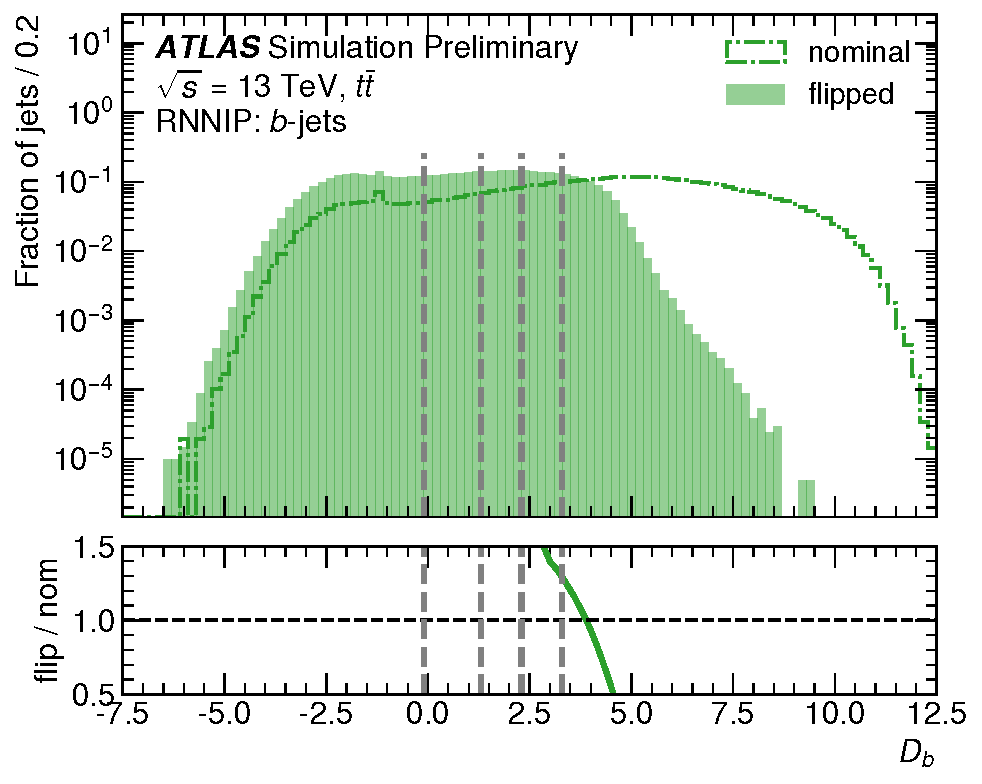
\includegraphics[width=0.41\linewidth]{\figpath/cf_$b$_disc_rnn_flip}
    }   
    \subfloat[]{ 
            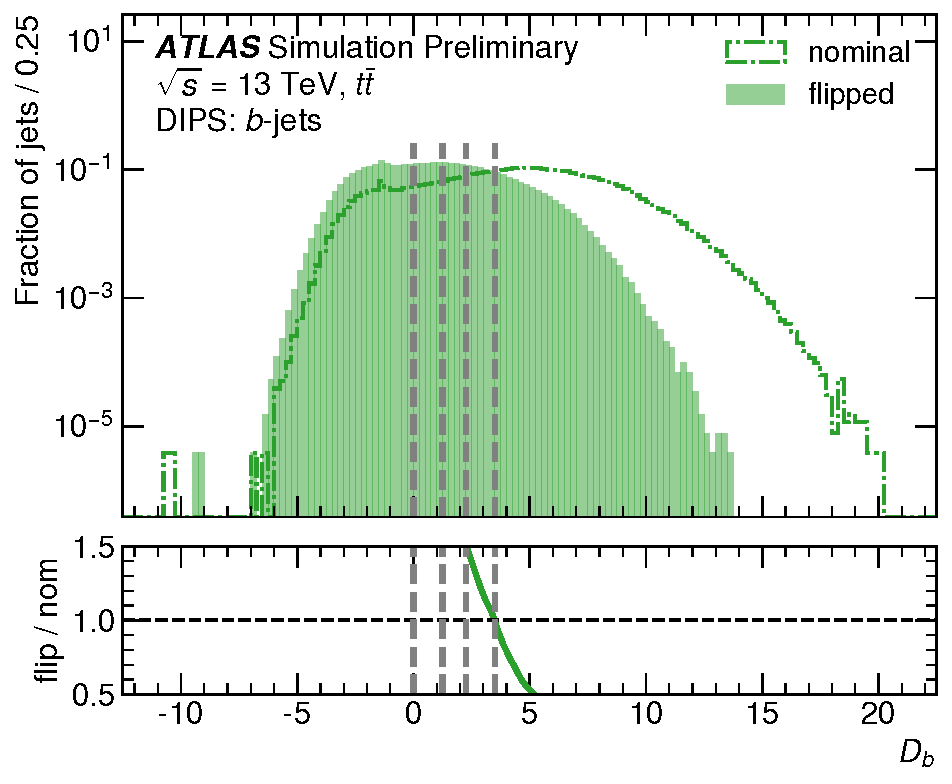
\includegraphics[width=0.4\linewidth]{\figpath/cf_$b$_disc_dips_flip}
    }   
    \caption{$D_b$ discriminant distributions for the nominal and flipped taggers. The vertical dashed lines correspond to the discriminant requirements for 85\%, 77\%, 70\% and 60\% inclusive $b$-jet efficiencies, corresponding to the efficiency benchmarks used at analysis level. Plots (a), (c) and (e) refer to the RNNIP performance, while (b), (d) and (f) refer to DIPS. Plots (a) and (b), (c) and (d), (e) and (f) show light-flavour jets, $c$-jets and $b$-jets respectively.}
    \label{fig:flippedDisc}
\end{figure}



%We quantify the decrease in $b$-efficiency for the flipped tagger by comparing the roc curves for the nominal and flipped taggers in Figure~\ref{fig:rocFlippedTaggers}. For this roc curve, the dashed lines showing the flipped taggers are better if the $l$-rej is lower for a fixed $b$-efficiency.  Although the performance of RNNIPFlip and DIPSFlip are comparable, DIPSFlip is not flipping quite as well as RNNIPFlip, presumably because the track ordering gives a larger difference for $b$-jets for RNNIPFlip.

%While the roc curves are our standard metric for algorithms we actually calibrate taggers in bins of the five bins for the $b$-effieciency: $> 85 \%$ (most $l$-jet like), $85\% - 77 \%$, $77\%-70\%$, $70\%-60\%$, and $ < 60\%$ (most $b$-jet like), and Table~\ref{table:} shows the efficiencies for $b$ and $l$-jets for each of the models of interest. The reason why the $l$-jet calibration is challenging is because of the need to constrain the fraction of HF jets passing a cut, and the bin that is most challenging is the bin with the most $b$-jets or the 60\% WP, which is the column in Table~\ref{tab:PCeff} of particular interest.
%Figure~\ref{fig:rocFlippedTaggers} and Table~\ref{tab:PCeff} both demonstrate that 

\begin{figure}[htpb!]
    \centering
    \subfloat[]{ 
            \includegraphics[width=0.48\textwidth]{\figpath/varyEff_RNNIP}%{flipAvgIter_l_flip}
    }   
    \subfloat[]{ 
            \includegraphics[width=0.48\textwidth]{\figpath/varyEff_DIPS}%{flipAvgIter_c_mistag_eff_l_rej_flip}%{flipAvgIter_c_flip}
    }   
    \caption{1 - Cumulative efficiency as a function of $b$-tagging discriminant for RNNIP (a) and DIPS (b). In both cases, the performance remains nearly unchanged for light-flavour jets when comparing nominal and flipped taggers, while the $b$-jet and $c$-jet efficiencies drop.}
    \label{fig:rocFlippedTaggers}
\end{figure}

\subsection{Track Selection Optimisation}
\label{subsec:optimisation}

%When DIPS is trained with the same inputs as RNNIP, DIPS achieves the the same performance whilst having training and evaluation times a factor of 2-4 times shorter than RNNIP. 
A major benefit of the reduced training time for DIPS is that it facilitates critical optimisation studies which require retraining the algorithm for each change one would like to examine. %As such, additional optimisations of the input features to the DIPS algorithm were examined. 
Two classes of optimisation are presented here: 1)~varying the selection of tracks given to DIPS for processing, and 2)~providing additional features per track. 

The DIPS implementation described so far relies on the same track selection as the IP3D and RNNIP algorithms. This selection, denoted \textit{nominal}, selects tracks with  
$\pT >1$~GeV, $|d_0|<1$~mm, ${|z_0 \sin \theta|<1.5}$~mm. This is a relatively strict selection that is used to keep the number mismeasured and pile-up tracks low, as the IP3D algorithm can be sensitive to such tracks. At the same time, this selection removes some of the key tracks from heavy flavour decays that are vital for classification. With the larger expressive power of the DIPS neural network over the IP3D model, DIPS will have more power to learn which tracks are useful for tagging and thus will potentially be less sensitive to such tracks. As a result, a \textit{loose} selection is examined, defined as $\pT >0.5$~GeV, $|d_0|<3.5$~mm, $|z_0 \sin \theta|<5$~mm, which utilises a lower $\pT$ threshold and a wider allowance on the impact parameter thresholds in order to capture more tracks from the heavy flavour decay. In addition, DIPS with the  \textit{loose} selection examines up to the 25 highest $s_{d_{0}}$ tracks, rather than 15 tracks as in the  \textit{nominal} selection, to further increase the ability to select tracks from heavy flavour decays. 

The average number of tracks of different origin per jet is shown in Table~\ref{table:trkComposition} for the \textit{nominal} and  \textit{loose} selections, and is shown separately per jet flavour. The total number of tracks ($n_{trk}$), the number of tracks from heavy flavour decays ($n_{trk}^{HF}$), the number of tracks from hadronisation, excluding those from heavy flavour decays ($n_{trk}^{hadr}$), and the number of tracks from mismeasurement, material interactions, and pile-up ($n_{trk}^{other}$), are compared. The \textit{loose} selection increases the average number of tracks per jet from heavy flavour decay by $\approx 15\%$ over the \textit{nominal} selection. However, for all flavours, the \textit{loose} selection also increases the number of fragmentation and other tracks per jet.  As can be seen in the ROC curves in Figure~\ref{fig:ip3d_cuts}, DIPS with the \textit{loose} selection (shown in pink) outperforms the nominal DIPS (shown in purple) by up to $\approx 40\%$ for light-flavour jet and charm jet rejection.

\begin{table}[htbp!]
  \begin{center} 
    \begin{tabular}{l | c | c | c | c | c } % 
      \textbf{Jet Flavour}         & \textbf{Track selection} & \textbf{$n_{trk}$} & \textbf{$n_{trk}^{HF}$} & \textbf{$n_{trk}^{hadr}$} & \textbf{$n_{trk}^{other}$}     \\
      \hline
      \multirow{2}{*}{$b$-jets} & \textit{nominal}      &  $5.9\pm2.7$ & $3.4\pm1.8$  & $2.0\pm1.9$ & $0.4\pm0.8$  \\
                                & \textit{loose}          &  $8.1\pm3.2$ &  $3.9\pm1.8$ &  $2.5\pm2.1$ &  $1.7\pm1.7$ \\
      \hline
      \multirow{2}{*}{ $c$-jets} & \textit{nominal}     &  $5.1\pm2.5$  &  $1.7\pm1.0$ & $2.9\pm2.2$ & $0.4\pm0.8$ \\
                                & \textit{loose}         &  $7.1\pm3.1$ &  $1.8\pm1.0$ & $3.6\pm2.4$ &  $1.7\pm1.7$ \\
      \hline
      {  Light-flavour}         & \textit{nominal}     &  $4.6\pm2.6$ &             -          & $4.1\pm2.5$ & $0.5\pm0.9$  \\
      {  jets}                  & \textit{loose}         &  $6.8\pm3.3$ &             -          & $5.0\pm2.7$ & $1.8\pm2.0$ \\
    \end{tabular}
    \caption{The average per jet total number of tracks ($n_{trk}$), the number of tracks from heavy flavour decays ($n_{trk}^{HF}$), the number of tracks from hadronisation, excluding those from heavy flavour decays ($n_{trk}^{hadr}$), and the number of tracks from mismeasurement, material interactions, and pile-up ($n_{trk}^{other}$), are shown for the \textit{nominal} and  \textit{loose} selections for each jet flavour.}
      \label{table:trkComposition}
  \end{center}
\end{table}

\begin{figure}[htbp!]
    \centering
    \subfloat[]{ 
            \includegraphics[width=0.48\textwidth]{\figpath/rocAvgIter_l_trkOpt}
    }   
    \subfloat[]{ 
            \includegraphics[width=0.48\textwidth]{\figpath/rocAvgIter_c_trkOpt}
    }   
    \caption{Light-flavour jet rejection as a function of $b$-jet efficiency (a) and $c$-jet rejection as a function of $b$-jet efficiency (b) of the nominal DIPS setup, DIPS with \emph{loose} track selection, and Optimised DIPS with the \emph{loose} track selection and additional IP inputs. The central curves and error bands show the mean and standard deviation, respectively, of the rejection at each $b$-jet efficiency for 5 trainings. The ratios are computed with respect to the DIPS ROC curve.}
    \label{fig:ip3d_cuts}
\end{figure}


\subsection{Optimised DIPS Performance}
\label{subsec:optimiseddips}

Beyond the \textit{loose} selection, the impact of adding more per-track features is also examined, namely the impact parameters $d_0$ and $z_0 \sin\theta$. 
%While the nominal set of features includes IP significance and kinematic features, this additional set breaks down the IP and kinematic information further.  
The DIPS with additional features and \textit{loose} track selection, denoted \textit{Optimised DIPS}, can be seen in orange in the ROC curves in Figure~\ref{fig:ip3d_cuts}, compared to a reference of the nominal DIPS or RNNIP trainings, respectively. 
For the following studies, Optimised DIPS is built with the same architecture described in Section~\ref{subsec:algdetails}.
%to the nominal DIPS training and the DIPS training with only the \textit{loose} track selection. 
The Optimised DIPS outperforms the nominal DIPS  by up to a factor of 2 in light-flavour jet rejection and a factor of 1.5 in the $c$-jet rejection.

While ROC curves give a global view of an algorithm's performance, the behavior of the $b$-tagging efficiency and the background rejection as a function of key kinematic variables is also vital to performance within analyses. 
To explore this metric, a threshold defining an inclusive 77\% $b$-tagging efficiency for each algorithm is determined, and the $b$-jet efficiency and background rejections with this fixed threshold are examined as a function of kinematic quantities. 
The $b$-jet efficiency as well as the $c$-jet and light-flavour jet rejections versus jet $\pT$ and $\eta$ are shown in Figure~\ref{fig:fixed77_pT_eta}, for the RNNIP, DIPS, and Optimised DIPS algorithms.  The behavior of DIPS and RNNIP are nearly the same across the $\pT$ and $\eta$ range, with DIPS providing a slightly higher light-flavour jet rejection. The Optimised DIPS delivers a factor of 1.5 to 2.5 in additional light-flavour jet rejection and up to $\approx33\%$ additional charm jet rejection. 
Loosening the track requirements for Optimised DIPS could potentially have the drawback of increasing the performance dependency on pile-up. 
We therefore check the $b$-jet efficiency, $c$-jet and light-flavour jet rejection as a function of the average number of proton-proton collisions per bunch crossing $\langle\mu\rangle$, also shown in Figure~\ref{fig:fixed77_pT_eta}. 
The Optimised DIPS performance dependency on $\langle\mu\rangle$ is not found to be significantly stronger than the baseline DIPS or RNNIP.

\begin{figure}[htbp!]
    \centering
          \subfloat[]{ 
    \centering
            \includegraphics[width=0.32\linewidth]{{{\figpath/b-eff_vs_pT77.0_std_ratio}}}
    }   
    \subfloat[]{
    \centering 
            \includegraphics[width=0.32\linewidth]{{{\figpath/b-eff_vs_eta77.0_std_ratio}}}
    }   
    \subfloat[]{
    \centering 
            \includegraphics[width=0.32\linewidth]{{{\figpath/b-eff_vs_avgmu77.0_std_ratio}}}
    }   
    \\
     \centering
    \subfloat[]{ 
    \centering
            \includegraphics[width=0.32\linewidth]{{{\figpath/l-rej_vs_pT77.0_std_ratio}}}
    }   
    \subfloat[]{
    \centering 
            \includegraphics[width=0.32\linewidth]{{{\figpath/l-rej_vs_eta77.0_std_ratio}}}
    }   
    \subfloat[]{
    \centering 
            \includegraphics[width=0.32\linewidth]{{{\figpath/l-rej_vs_avgmu77.0_std_ratio}}}
    }   
    \\
    
    \subfloat[]{ 
    \centering
            \includegraphics[width=0.32\linewidth]{{{\figpath/c-rej_vs_pT77.0_std_ratio}}}
    }   
    \subfloat[]{ 
    \centering
            \includegraphics[width=0.32\linewidth]{{{\figpath/c-rej_vs_eta77.0_std_ratio}}}
    }    
    \subfloat[]{
    \centering 
            \includegraphics[width=0.32\linewidth]{{{\figpath/c-rej_vs_avgmu77.0_std_ratio}}}
    }   \caption{Performance plots using a fixed cut with 77\% $b$-jet efficiency. Plots (a), (b) and (c) show the $b$-jet efficiency as a function of jet $\pT$, $\eta$ and average number of proton-proton collisions per bunch crossing $\langle\mu\rangle$. Plots (d), (e) and (f) show the light-flavour rejection as a function of the same quantities, while plots (g), (h) and (i) show the $c$-jet rejection.}
    \label{fig:fixed77_pT_eta}
\end{figure}


One challenge in comparing background rejections with a fixed threshold is that the $b$-tagging efficiency is not the same for each algorithm in each kinematic region. 
As an alternative, the threshold on the $b$-tagging discriminant can be tuned in each kinematic region to give a constant 77\% $b$-tagging efficiency. 
A comparison of the $c$-jet and light-flavour jet rejections as a function of $\pT$ and $\eta$ for the DIPS, RNNIP, and Optimised DIPS algorithms with flat 77\% $b$-tagging efficiency can be seen in Figure~\ref{fig:flat77_pt_eta}. 
While DIPS and RNNIP are seen to be quite similar, DIPS provides up to $\approx 20\%$ additional light-flavour jet rejection in some regions of jet $\pT$. The Optimised DIPS shows more than a factor of 2 increase in light-flavour jet rejection and up to $\approx 50\%$ additional charm jet rejection of the DIPS, for jets with $\pT$ between 50 and 300~GeV.

\begin{figure}[htbp!]
    \centering
    \subfloat[]{ 
\centering
            \includegraphics[width=0.48\textwidth]{{{\figpath/l-rej_vs_pT_flatEff77.0_std_ratio}}}
    }   
    \subfloat[]{
    \centering 
            \includegraphics[width=0.48\textwidth]{{{\figpath/l-rej_vs_eta_flatEff77.0_std_ratio}}}
    }   \\
    
    \subfloat[]{ 
    \centering
            \includegraphics[width=0.48\textwidth]{{{\figpath/c-rej_vs_pT_flatEff77.0_std_ratio}}}
    }   
    \subfloat[]{ 
    \centering
            \includegraphics[width=0.48\textwidth]{{{\figpath/c-rej_vs_eta_flatEff77.0_std_ratio}}}
    }   

    \caption{Performance plots using a requirement where the $b$-jet efficiency is 77\% in each bin. Plots (a) and (b) show the light-flavour rejection as a function of jet $\pT$ and $\eta$, while plots (c) and (d) show the $c$-jet rejection as a function of the same quantities.}
    \label{fig:flat77_pt_eta}
\end{figure}




%\input{Run 3 taggers}

\chapter{Statistical techniques}
\chapter{Analysis selection}
\chapter{Background estimation}
\chapter{Results}
\chapter{Future directions?}
\chapter{Conclusions}

\appendix
\chapter{Reweighting loss function}
\chapter{Further statistics fundamentals}
\chapter{Gaussian Processes}
\chapter{ML for jet $\rightarrow$ parton assignment}


...
\bibliographystyle{plain}
\bibliography{mybib}
\end{document}